% --- Style du Document ---
\documentclass[a4paper]{article}

% --- Packages ---
\usepackage{geometry}
\usepackage{fancyhdr}
\usepackage{float}
\usepackage{graphicx}
\usepackage{lastpage}
\usepackage{hyperref}
\usepackage{tocbibind}
\usepackage{xcolor}
\usepackage{color, colortbl}
\usepackage{array,booktabs}
\usepackage[figurename=Fig.]{caption}

% --- Style du Document ---
\geometry{top=2cm, bottom=2cm, left=2cm, right=2cm}
\geometry{headsep=9ex}
\pagestyle{fancy}
\fancyhf{}
\renewcommand\refname{Bibliographie}
\definecolor{Gray}{gray}{0.9}

% --- Style de l'en-tête ---
\lhead{
\includegraphics[height=0.8cm, page=1]{Images/Logos/logoinsa.pdf}}
\renewcommand{\sectionmark}[1]{\markboth{\thesection\ #1}{\rightmark}}
\chead{
\includegraphics[height=1.2cm, page=1]{Images/Logos/logolamih.png}}
\rhead{
\includegraphics[height=1.2cm, page=1]{Images/Logos/logouphf.pdf}}
%\chead{\sffamily\small\leftmark}
\renewcommand{\headrulewidth}{1pt}

% --- Style du pied de page ---
\lfoot{PLP23INT16 : Lattybrides}
\cfoot{}
\rfoot{Page \thepage / \pageref{LastPage}}
\cfoot{\sffamily\small\leftmark}
\renewcommand{\footrulewidth}{0.4pt}

% --- Document ---
\begin{document}
	% --- Page de Garde ---
	\begin{titlepage}
		\begin{center}
			% Logos
			
			\begin{table}[h]
			\centering
				\begin{tabular}{c c c}
					
\includegraphics[width=4cm]{Images/Logos/logoinsa.pdf} \hspace{1.5cm} & 
\includegraphics[width=4cm]{Images/Logos/logolamih.png} & \hspace{1.5cm} 
\includegraphics[width=4cm]{Images/Logos/logouphf.pdf} \\
				\end{tabular}
			\end{table}
			\vspace{1cm}
		
			\textsc{\LARGE INSA Hauts-de-France}\\[2cm]
			
			% Titre
			\rule{16cm}{0.8pt}
			{\\[0,8cm] \huge \bfseries Étude de la capacité d'adsorption de différentes structures lattices hybrides avec des gradients de réseaux}\\
			\vspace{0,5cm}
			{\Large \bfseries PLP23INT16}\\[0,5cm]
			\rule{16cm}{0.8pt}
			\textsc{\\[0,5cm]Février 2024}
			\vspace{2cm}
			
			% Image de la page de garde
			\begin{figure}[H]
				\centering
				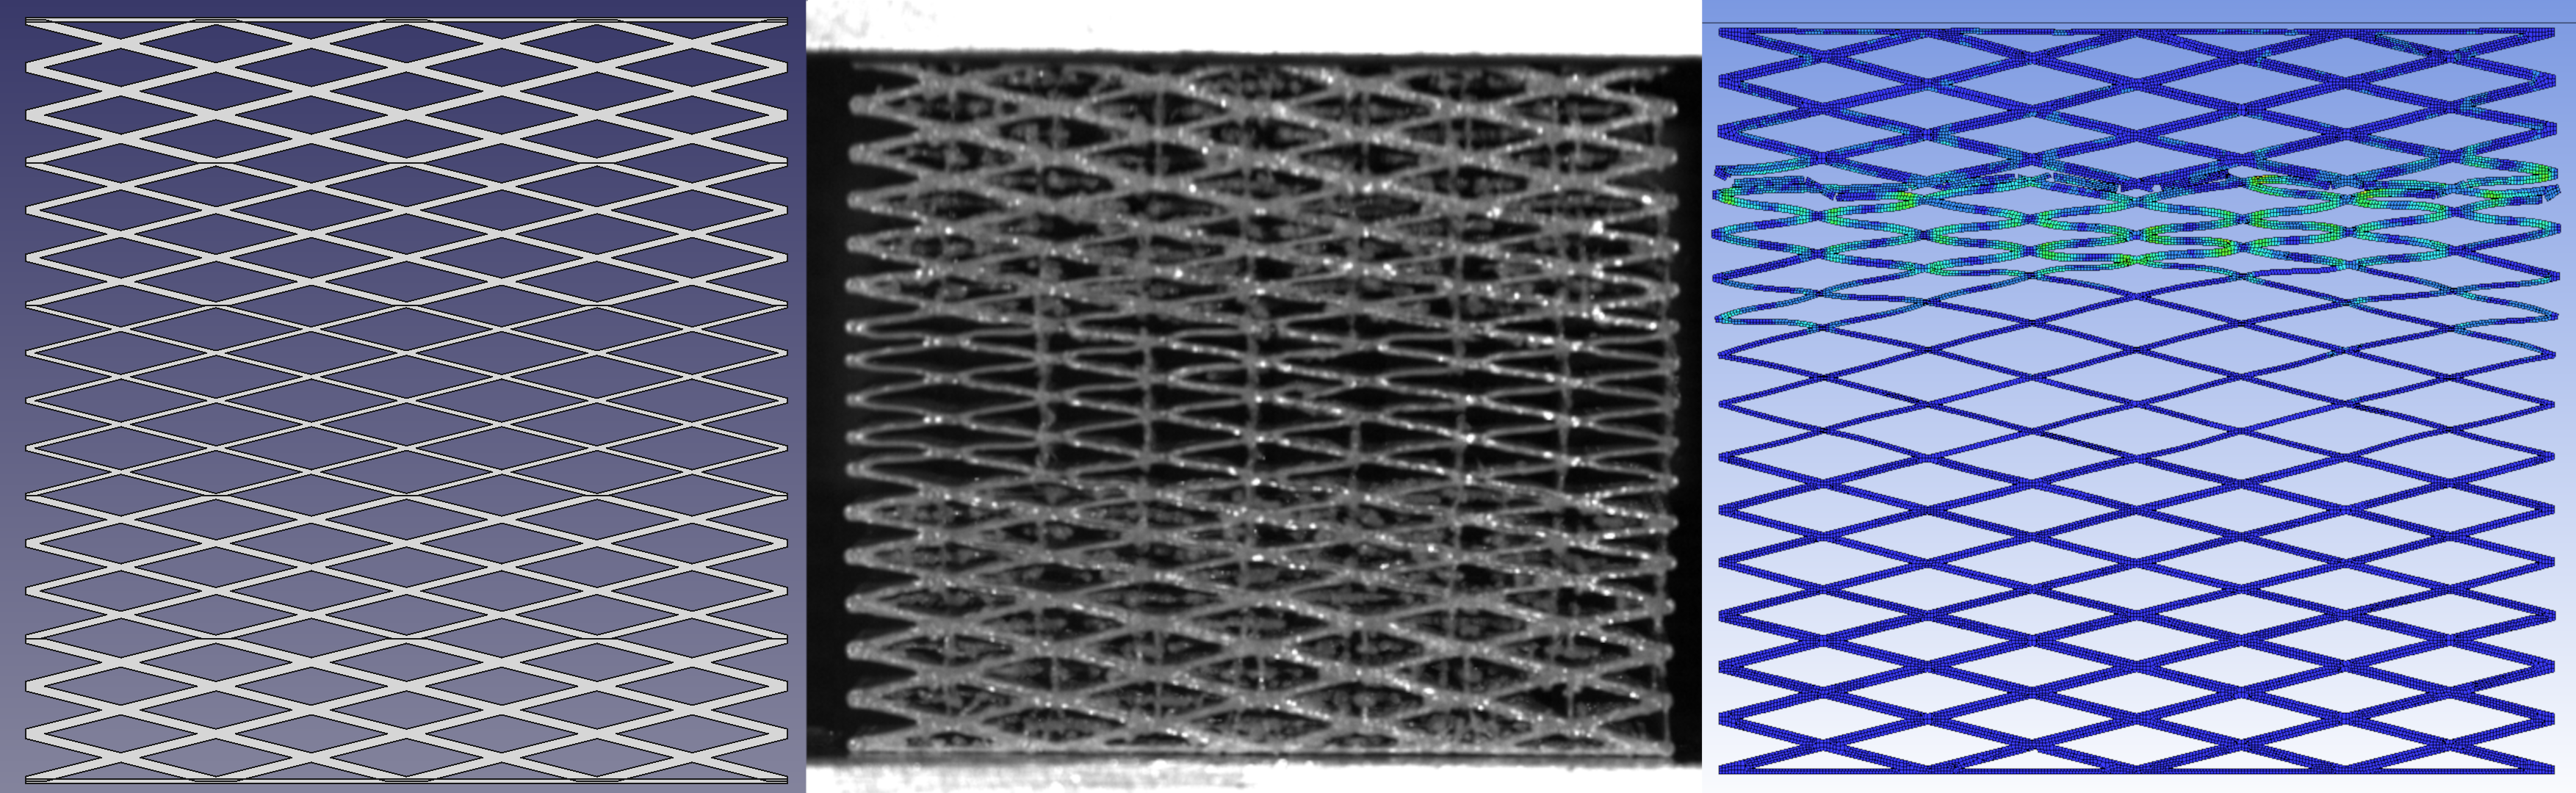
\includegraphics[width=16.5cm]{Images/page_garde/page_garde.png}
			\end{figure}
			\vspace{3cm}
		
			% Auteur et Professeur
			\begin{minipage}{1\textwidth}\large
				\textsc{Bacout Valentin}\\
				\textsc{Benhilal Salma}\\
				\textsc{Bossu Romain}\\
				\textsc{\underline{Herman Adrien}}
				\begin{flushright}
				\textsc{{Professeurs : M. Delille \& M. Lauro}}
				\end{flushright}
			\end{minipage}
		\end{center}
	\end{titlepage}
	
	% --- Remerciements ---
	\section*{Remerciements}
	
	\hspace{0.5cm}Avant de commencer la rédaction de ce rapport d'expérience, nous tenions tout d’abord à remercier Rémi Delille et Frank Lauro, nos tuteurs. Votre expertise, votre patience et votre soutien nous ont été d'une aide inestimable durant ces 6 derniers mois. Grâce à vos conseils éclairés, nous avons pu approfondir nos connaissances et réaliser un travail dont nous sommes fiers. Merci également à vous pour votre disponibilité.\\
	
	Nous souhaitons par ailleurs adresser nos remerciements à Bernard Philippe et Jean-Hubert Anceau, nos enseignants, pour leurs conseils avisés.\\
	
	Plus généralement, nous remercions l’ensemble du LAMIH pour leur accueil chaleureux et leur financement.\\
	
	\begin{flushright}
		Salma BENHILAL, Valentin BACOUT,
		
		Romain BOSSU, Adrien HERMAN
	\end{flushright}
	
	\section*{Remerciements du chef d'équipe}
	
	\hspace{0.5cm}Je tiens également à remercier l'équipe du PLP Lattybrides, Salma BENHILAL, Valentin BACOUT et Romain BOSSU, sans qui ce projet n'aurait pas abouti. Le travail à leurs côtés a été très agréable et chaque personnes de l'équipe a su ajouter sa brique à l'édifice. Je suis conscient que la programmation n'est pas le domaine de prédilection de l'équipe, mais nous avons su nous former et réaliser nos objectifs pour générer nos structures lattices.\\
	
	\begin{flushright}
		\textbf{\large Bravo à tous et merci !}
		
		Adrien HERMAN
	\end{flushright}
	
	\vspace{3cm}
	
	\section*{Liens utiles}
	\begin{itemize}
		\item Lien du drive du projet (Autorisation de lecture et d'écriture) :\\ \href{https://drive.google.com/drive/folders/1Y3JJd3HjbAqBD-ykjscEf51ELvaYXhEQ?usp=sharing}{https://drive.google.com}
		\item Lien du dossier du drive où sont stockées toutes les structures testées :\\
		\href{https://drive.google.com/drive/folders/1Dxy5Yaq-WHseOIPNWpTo1YhIdbHROOMq?usp=drive_link}{https://drive.google.com}
		\item Lien du dossier du drive où sont stockées toutes les données expérimentales et les images de la caméra à grande vitesse :\\
		\href{https://drive.google.com/drive/folders/1GixQ5m0--2UXGmWGoiHR0oR_ZuMvKeyD?usp=drive_link}{https://drive.google.com}
		\item Lien du GitHub Lattybrides (Code source de l'Atelier \textit{FreeCAD} pour la génération des structures) :\\ \href{https://github.com/AdrienHerman/Lattybrides/tree/main}{https://github.com/AdrienHerman/Lattybrides}
		\item Lien du GitHub TDC (Code source du logiciel de Traitement des Données) :\\ \href{https://github.com/AdrienHerman/TDC-Traitement_des_Donnees_de_Crash}{https://github.com/AdrienHerman/TDC}
		\item Lien vers la dernière version compilée du logiciel de Traitement des Données de Crash (TDC) :\\ \href{https://github.com/AdrienHerman/TDC-Traitement_des_Donnees_de_Crash/releases/tag/TDC_2_2}{https://github.com/AdrienHerman/TDC\_2\_0}
	\end{itemize}
	
	% --- Table des Matières ---
	\newpage
	\renewcommand*\contentsname{Table des matières}
	\tableofcontents
	\newpage
	
	% --- Tables des Illustrations ---
	\newpage
	\renewcommand{\listfigurename}{Table des illustrations}
	\listoffigures
	\captionsetup{justification=centering}
	\newpage
	\renewcommand{\listtablename}{Liste des tableaux}
	\listoftables
	\captionsetup{justification=centering}
	\newpage
	
	\section{Introduction}
	\hspace{0.5cm}Dans un environnement industriel de plus en plus concurrentiel, les entreprises cherchent continuellement des stratégies pour rester à la pointe et surpasser leurs rivaux. Avec la croissance de la demande d’économie d’énergie, l'intérêt pour les pièces légères s'intensifie également. Par exemple, dans l'industrie automobile, alléger le poids des voitures favorise l'économie de carburant. Face à ce besoin, la mise en \oe uvre des structures en treillis ont provoqué un changement de point de vue, en particulier dans la quête des systèmes d'absorption d’énergie efficace. En effet, les structures en treillis (lattices) représentent une catégorie de structures mécaniques dont la géométrie est caractérisée par une répétition de motifs tout en ayant un taux de porosité d'au moins $70\%$. Ces caractéristiques offrent des propriétés mécaniques avantageuses, telles que l’absorption d’énergie dans le cas d’un crash. La fabrication de ces structures a été facilitée par l’évolution des techniques de fabrication additive qui permet la production de géométries complexes dans les trois dimensions.
	\newpage
	
	\section{État de l'Art}
	\subsection{Structures Lattices homogènes}
	\hspace{0.5cm}Commençons par expliquer ce qu’est une structure lattice. Une structure lattice est une structure treillis de minimum 70\% de taux de porosité. Ces treillis permettent de créer des pièces légères tout en gardant une rigidité élevée. Certaines géométries de structures lattices sont aussi utilisées pour des propriétés d’absorption d’énergie. Elles peuvent aussi trouver leur place dans des domaines d’applications thermiques ou acoustiques. Les propriétés mécaniques de ces structures sont très dépendantes de leur géométrie et de leur densité.\\
	
	Pour fabriquer ces structures treillis, des techniques basées sur le pliage et le découpage de tôles métalliques existent. Cependant, ces techniques sont difficiles à mettre en place et ne
	permettent pas de fabriquer toutes les géométries possibles. Ces limitations sont principalement dues aux géométries en trois dimensions des structures lattices.\\
	
	Les technologies de fabrication additive ont cependant grandement facilité la production des structures en treillis. La plupart des études menées sur des structures lattices utilisent des méthodes d'impression 3D métallique. Parmi elle ont retrouve notamment les technologies Laser Beam Melting\footnote{Technologie LBM : Une fine couche de poudre métallique est fondue par un faisceau laser.} et Electron Beam Melting\footnote{Technologie EBM : Une fine couche de poudre métallique est fondue par un faisceau d'électrons.} qui permettent de fondre couche par couche un lit de poudre métallique. Dans le cadre de ce projet, la technique de fabrication Fused Deposition Modeling a été utilisée (\ref{imp_3D}).\\
	
	Ces architectures sont majoritairement utilisées pour des applications mécaniques notamment pour l'allègement de structures et l'absorption d'énergie en cas d'impact. On peut par exemple les retrouver dans des casques ou encore dans les tableaux de bords de voiture\footnote{Lors de la fabrication des tableaux de bords de voiture par injection plastique, la phase de compression est suivie par une phase de léger retrait formant ainsi une mousse et allégeant la pièce finale.}. Les structures lattices se retrouvent également en architecture et dans des applications artistiques car ce sont des structures jugées très esthétiques.
	
	\begin{figure}[H]
		\centering
		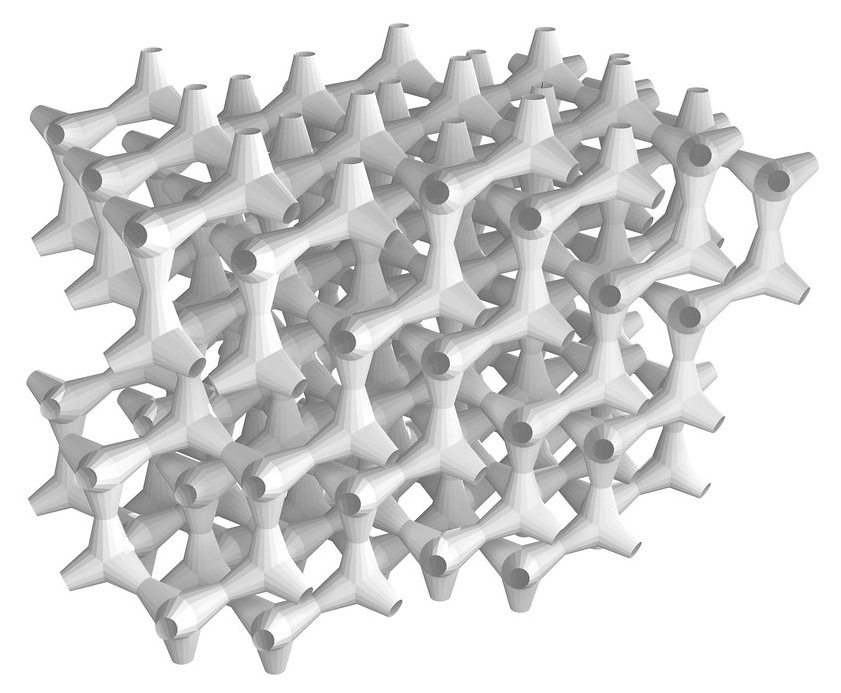
\includegraphics[height=5cm]{Images/2/lattice.jpg}
		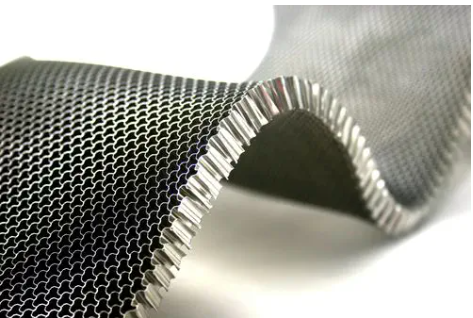
\includegraphics[height=5cm]{Images/2/nidabeille.png}
		\caption{Exemple de deux structures lattices homogènes. À gauche la structure est inspirée d'un réseau de modécules \cite{lat_hom1}. À droite la structure est une âme en nid d'abeille utilisé dans l'aéro-spatial \cite{lat_hom2}.}
	\end{figure}
	\newpage
	
	\subsection{Structures Lattices à gradient de réseau}
	
	\hspace{0.5cm}Dans le contexte de la recherche avancée dans des structures absorbantes d'énergie, les structures lattices à gradients de réseaux représentent une innovation permettant une manipulation précise des propriétés mécaniques à partir d’une architecture variable. Cette géométrie intègre des variations contrôlées ou non de propriétés structurelles du treillis ou de densité des cellules à travers le volume du matériau. Ces structures visent à optimiser la distribution des contraintes et l’absorption de l'énergie dans des contextes de crash.\\
	
	Les os sont des exemples remarquables de structures à gradients de réseaux dans la nature. Ils présentent une variation graduelle de densité, allant de la partie compacte externe à la structure spongieuse interne, optimisant ainsi la résistance et la légèreté.\\
	
	Le pomelo est également un bon exemple de structure lattice à gradient de réseau. En effet, ce fruit poussant en haut d'un arbre possède un treillis de plus en plus dense vers le cœur, protégeant ainsi le fruit lors de sa chute de l'arbre.
	
	\begin{figure}[H]
		\centering
		\includegraphics[height=7cm]{Images/2/os.png}
		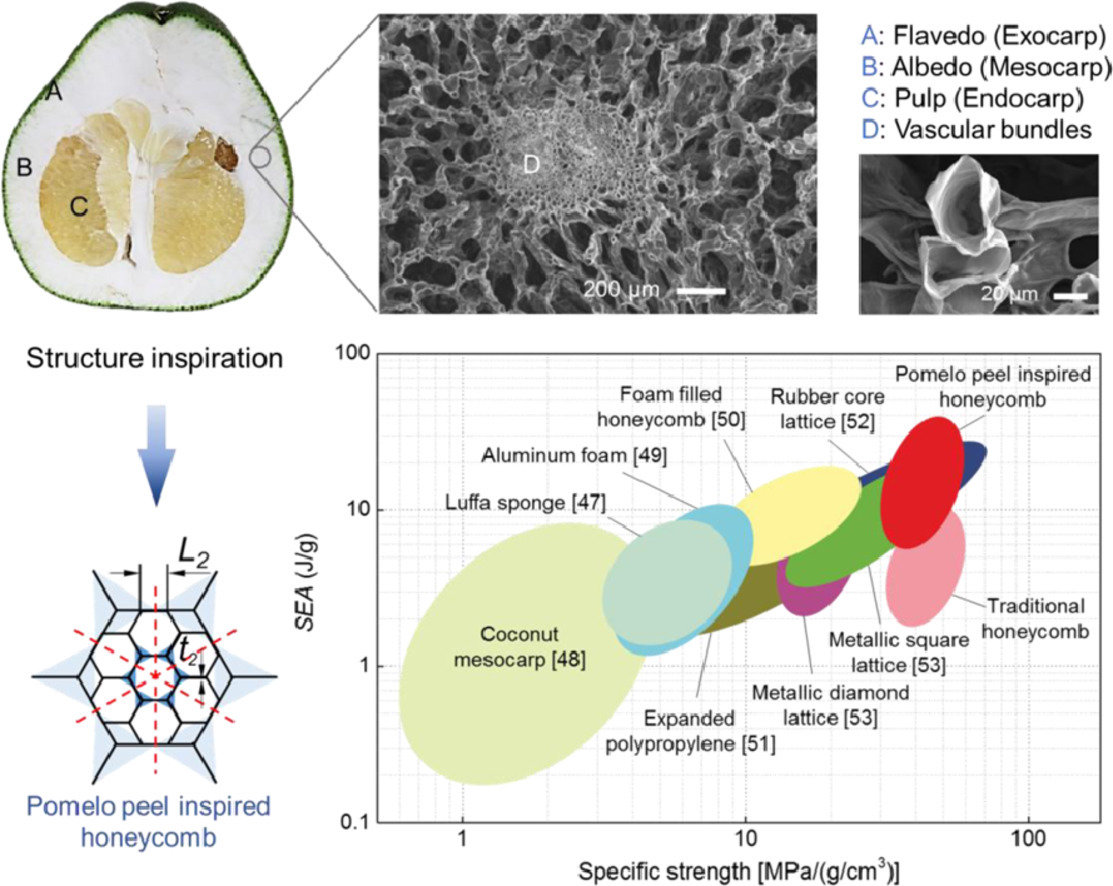
\includegraphics[height=7cm]{Images/2/pomelo.jpg}
		\caption{Illustration des treillis à gradient de réseau dans les os \cite{os} à gauche et dans le pomelo \cite{pomelo} à droite.}
	\end{figure}
	\newpage
	
	\section{Problématique}
	\hspace{0.5cm}Notre projet se base donc sur les deux constats précédemment établis. Les structures lattices homogènes permettent une légèreté des structures, très recherchée actuellement, et la nature possède des structures lattices à gradients de réseaux qui permettent une meilleure absorption d’énergie. Ces dernières sont néanmoins totalement aléatoires. La nécessité de pouvoir concevoir des structures lattices à gradient de réseau contrôlé est donc essentielle.\\
	
	Nous nous sommes donc questionnés sur l’apport de gradients de réseaux contrôlés au sein d’une structure lattice, en termes d’absorption d’énergie. Nous cherchons donc à comprendre :
	
	\begin{center}
		\centering{\textit{\Large En quoi les gradients de réseau améliorent-ils le comportement de structures lattices en crash ?}}
	\end{center}
	
	Notre but est d'absorber $20\%$ d'énergie en plus par rapport à une structure lattice homogène de référence.
	\newpage
	
	\section{Développement et Fabrication des Structures}
	\subsection{Méthode de génération des structures}
	\hspace{0.5cm}Dans le but de générer nos structures, plusieurs solutions s’offraient à nous. Dans un premier temps, nous avons cherché un logiciel / une extension \textit{Python} existante ce qui aurait pu nous faire gagner un temps non négligeable. Grâce à ce logiciel / cette extension, nous aurions pu générer des structures rapidement mais nous n’aurions pas eu la liberté de création de géométrie que nous désirions, ni la possibilité d’ajouter des gradients. De plus, nous n’aurions pas pu obtenir des structures à masse constante, ce qui est indispensable afin d’avoir une étude dans les mêmes conditions d’expérimentation (voir \ref{variables_etude}). Certains logiciels existent sur le marché mais n’étaient pas adaptés à nos besoins et sont payants. L’achat d’une licence n’était pas envisageable dans le cadre de ce projet.\\
		
	Nous avons réfléchi à l’éventualité de concevoir les structures manuellement, à l’aide d’un logiciel de modélisation 3D comme \textit{Catia V5} ou \textit{SolidWorks}. Cette éventualité nous aurait permis de générer des structures facilement et d’être assez libre pour la création de géométries diverses. Cependant, il aurait été difficile voire impossible de contrôler la masse des structures. La tâche de conception aurait également été longue et fastidieuse.\\
		
	Notre dernière solution était de développer une extension \textit{FreeCAD} de génération de structures automatisée. Pourquoi utiliser le modeleur 3D \textit{FreeCAD} ? Ce modeleur 3D est essentiellement développé en \textit{Python} et en \textit{C}. Son code est également open-source\footnote{Open-Source = En libre accès} et permet l’ajout d’extension (d’atelier) utilisant les fonctionnalités existantes du logiciel et d’ateliers tierces. Cette solution nous permet de rester totalement libre sur la création de géométrie moyennant le temps de développement en \textit{Python}. Nous pouvons également contrôler facilement la masse de nos structures via un algorithme d’optimisation simple. L’introduction de gradients dans des géométries de base peut se faire de manière très simple. Étant donné que nous avons un script nous permettant de générer une structure de référence, il nous suffit d’appeler ce script une fois par couche de gradient. L'utilisation de l'atelier développé est décrite dans l'Annexe 1 (\ref{annexe1}).
	\newpage
	
	\subsection{Algorithme d'optimisation de masse}
	\hspace{0.5cm}Nos essais doivent obligatoirement se dérouler dans les mêmes conditions. En effet, si plusieurs paramètres de l’étude varient en même temps, aucune conclusion ne pourra être tirée des données récoltées. La masse de la structure fait partie des conditions d’expérimentation et est directement liée à l’épaisseur des parois de la structure ainsi que le taux de porosité de celle-ci. Le taux de porosité est un paramètre utilisateur qui ne doit pas être modifié automatiquement par le script d’optimisation. En revanche, l’épaisseur des parois peut-être légèrement modifiée afin d’obtenir une masse cible.\label{masse}\\
	
	\underline{L’algorithme d’optimisation utilisé est très basique et voici un logigramme représentant son fonctionnement :}\\
	
	\begin{figure}[H]
		\centering
		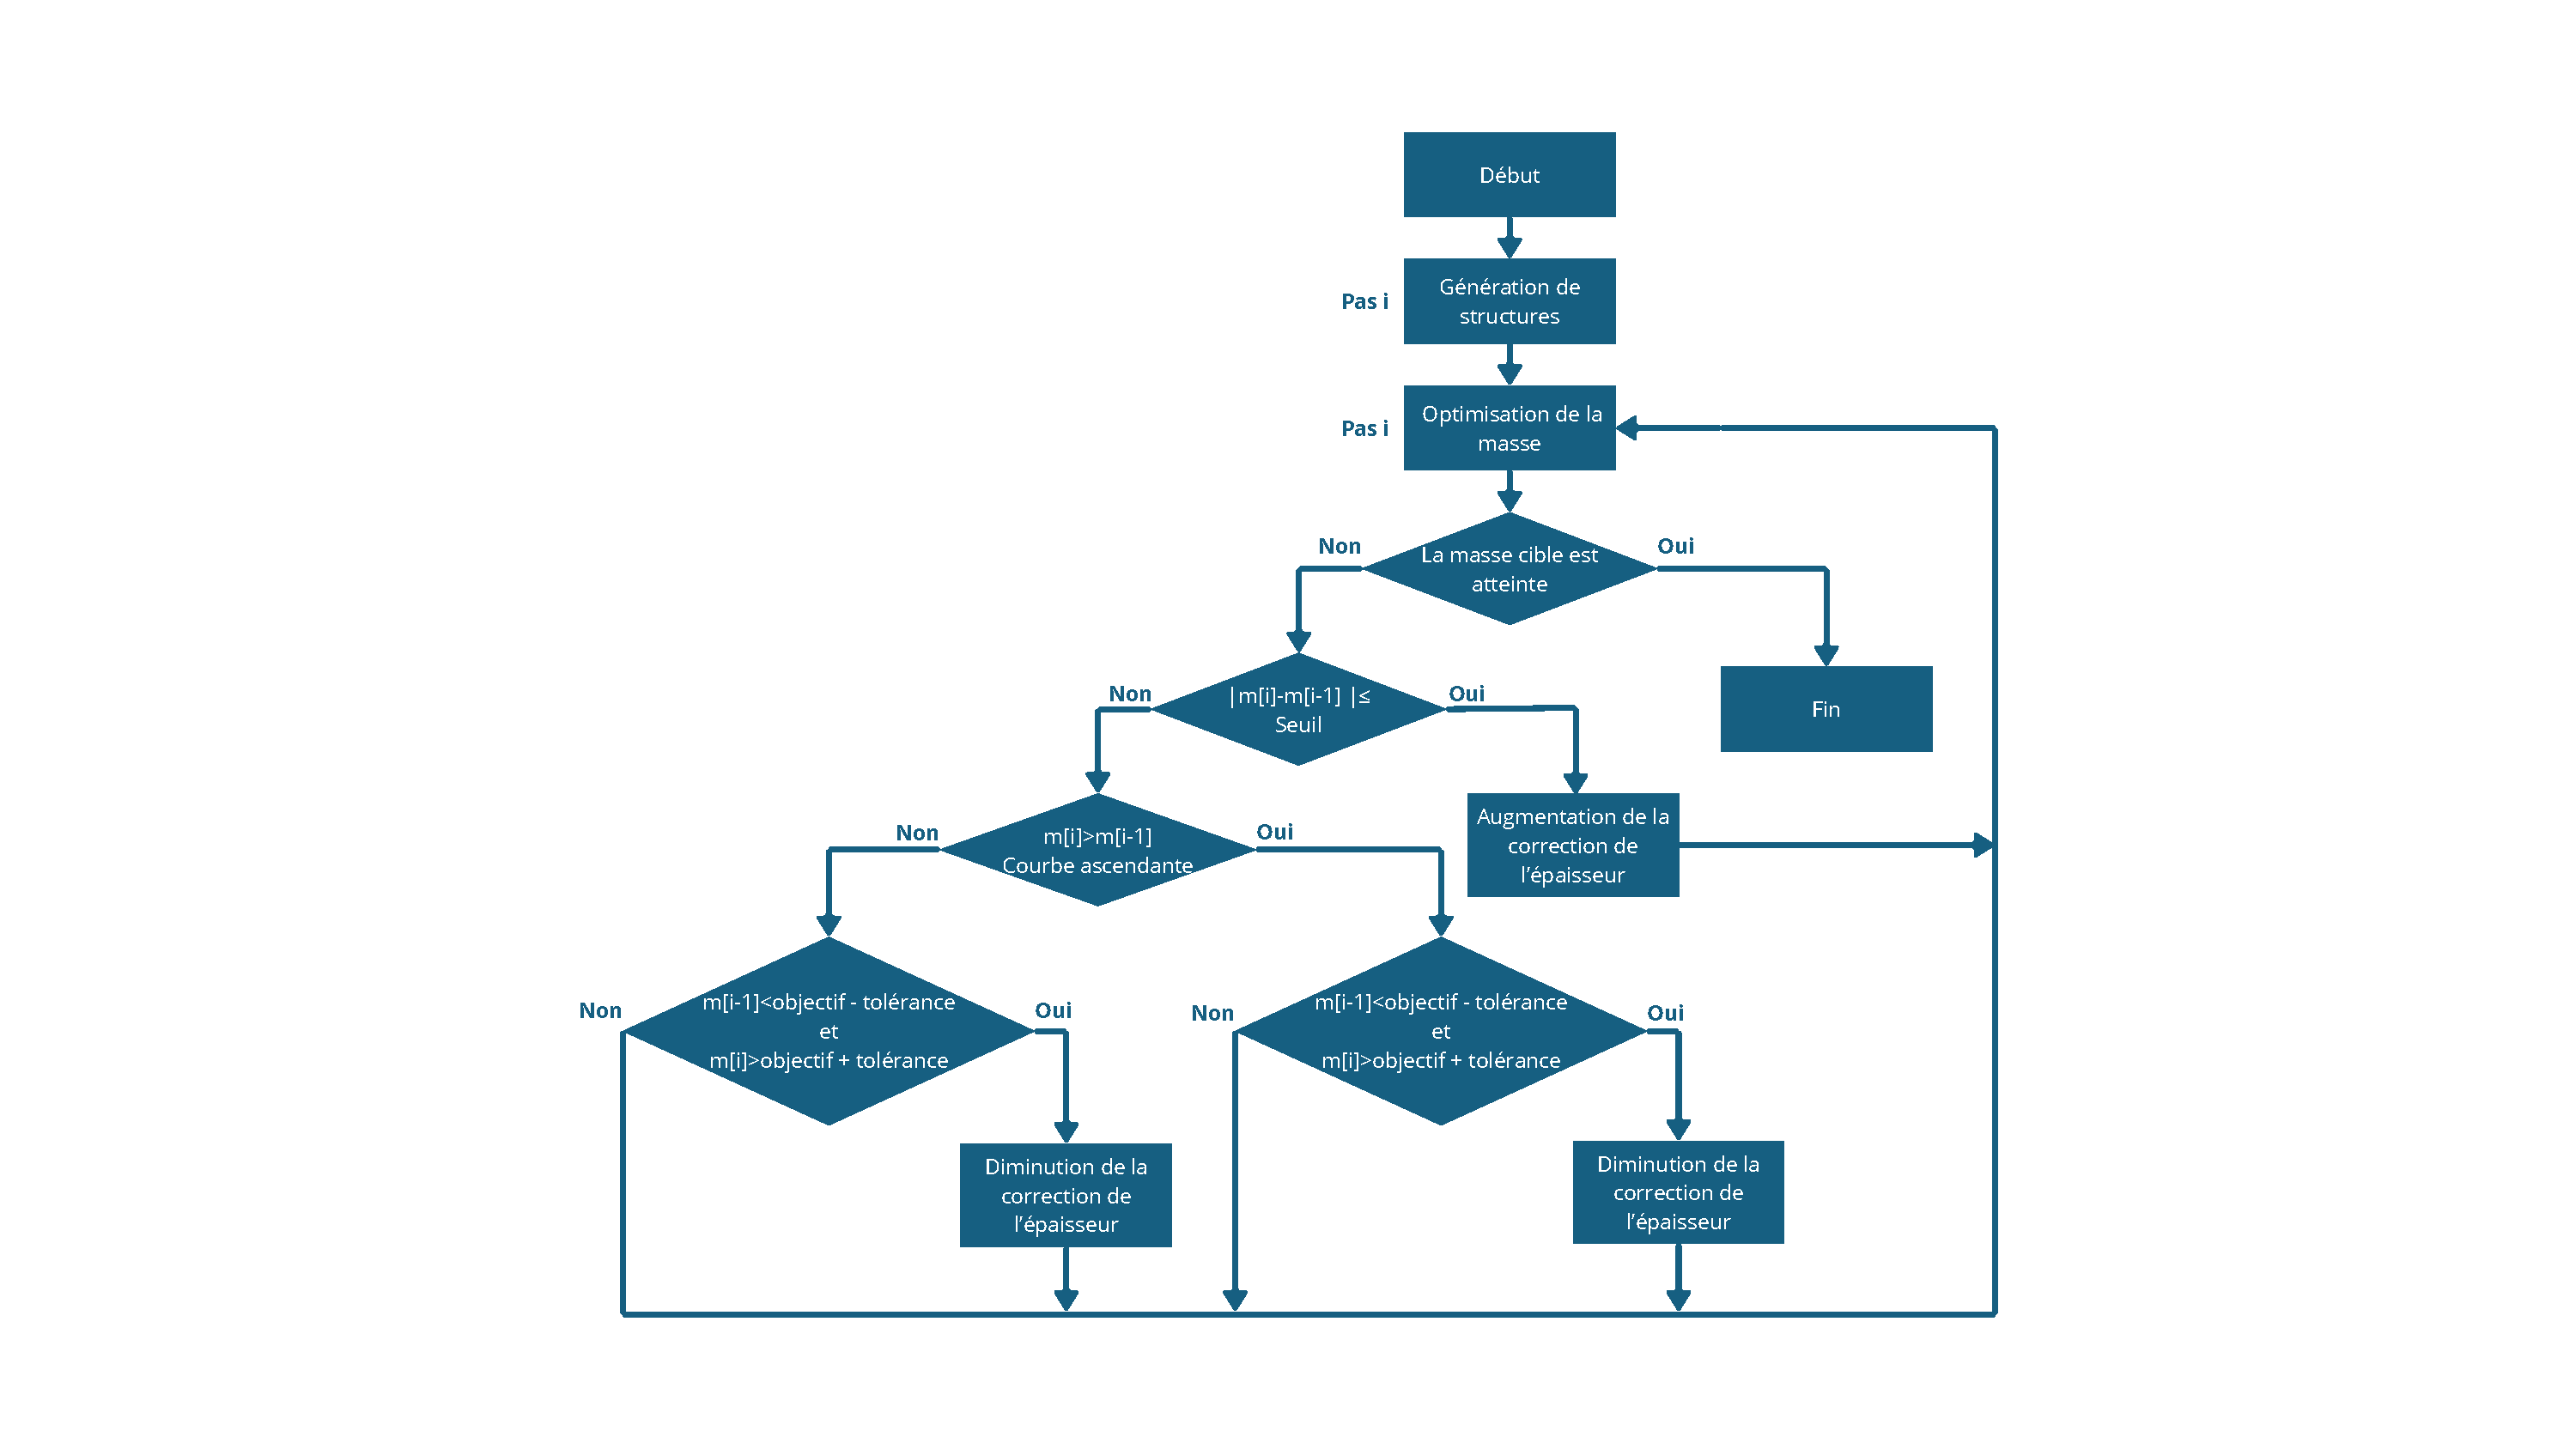
\includegraphics[width=16.5cm]{Images/4/log_opti_masse.pdf}\\
		\caption{Logigramme décrivant l'algorithme d'optimisation de la masse}
	\end{figure}
	\newpage

	\underline{Cet algorithme est composé de trois variables principales :}
	
	\begin{itemize}
		\item $ep$ : L’épaisseur des parois de la structure.
		\item $\Delta ep$ : Variable décrivant la quantité d’épaisseur à modifier à chaque pas de calcul.
		\item $fact_{\Delta ep}$ : Pourcentage d’augmentation / diminution de $\Delta ep$
	\end{itemize}

	Le fonctionnement est simple, si la masse actuelle de la structure est inférieure à la masse cible, $ep$ sera augmentée de $\Delta ep$. Cependant, il est possible que la variation d’épaisseur $\Delta ep$ engendre une trop grande augmentation de la masse (\ref{trop_grande_aug_ep}). Dans ce cas, $\Delta ep$ doit être diminuée afin de converger : $\Delta ep_{i+1} = (1 - fact_{\Delta ep}) * \Delta ep_{i}$.\\
	
	Dans le but d’améliorer la convergence de l’algorithme, donc de réduire le temps de calcul, l’algorithme est également autorisé à augmenter $\Delta ep$ si la variation de la masse est inférieure à un certain seuil : $\Delta ep_{i+1} = (1 + fact_{\Delta ep}) * \Delta ep_{i}$.
	
	\begin{figure}[H]
		\centering
		\includegraphics[height=8cm]{Images/4/tolerance.pdf}\\
		\caption{Phénomène de dépassement de l'objectif de masse à atteindre si l'augmentation de l'épaisseur des parois est trop grande}
		\label{trop_grande_aug_ep}
	\end{figure}
	\newpage
			
	\subsection{Méthode d'impression des structures}
	\subsubsection{Principe de la technologie FDM}
	\hspace{0.5cm}Les structures lattices ont certes de grandes propriétés en allègement des systèmes mécaniques et en crash, mais sont malheureusement compliquées à produire. En effet, les méthodes de fabrication classiques (tournage, fraisage, etc…) permettent la fabrication de pièces de formes complexes, mais sont limités par le passage des outils d’enlèvement de matière.\\
	
	Depuis les années 90, une nouvelle méthode de fabrication révolutionnaire est apparue. Cette méthode n’utilise pas un procédé d’enlèvement de matière, mais d’ajout de matière. Nous l’appelons la fabrication additive ou encore impression 3D. Le principe de la fabrication additive est de pouvoir produire un volume couche par couche en ajoutant de la matière qui peut se présenter sous plusieurs formes (Résines photosensibles, poudres, filaments, etc…). La technologie de fabrication additive utilisée dans le cadre de ce projet est l’impression 3D FDM \label{imp_3D}\footnote{Fused Deposition Modeling ou en français : Dépôt de fil fondu}.
	
	\begin{figure}[H]
		\centering
		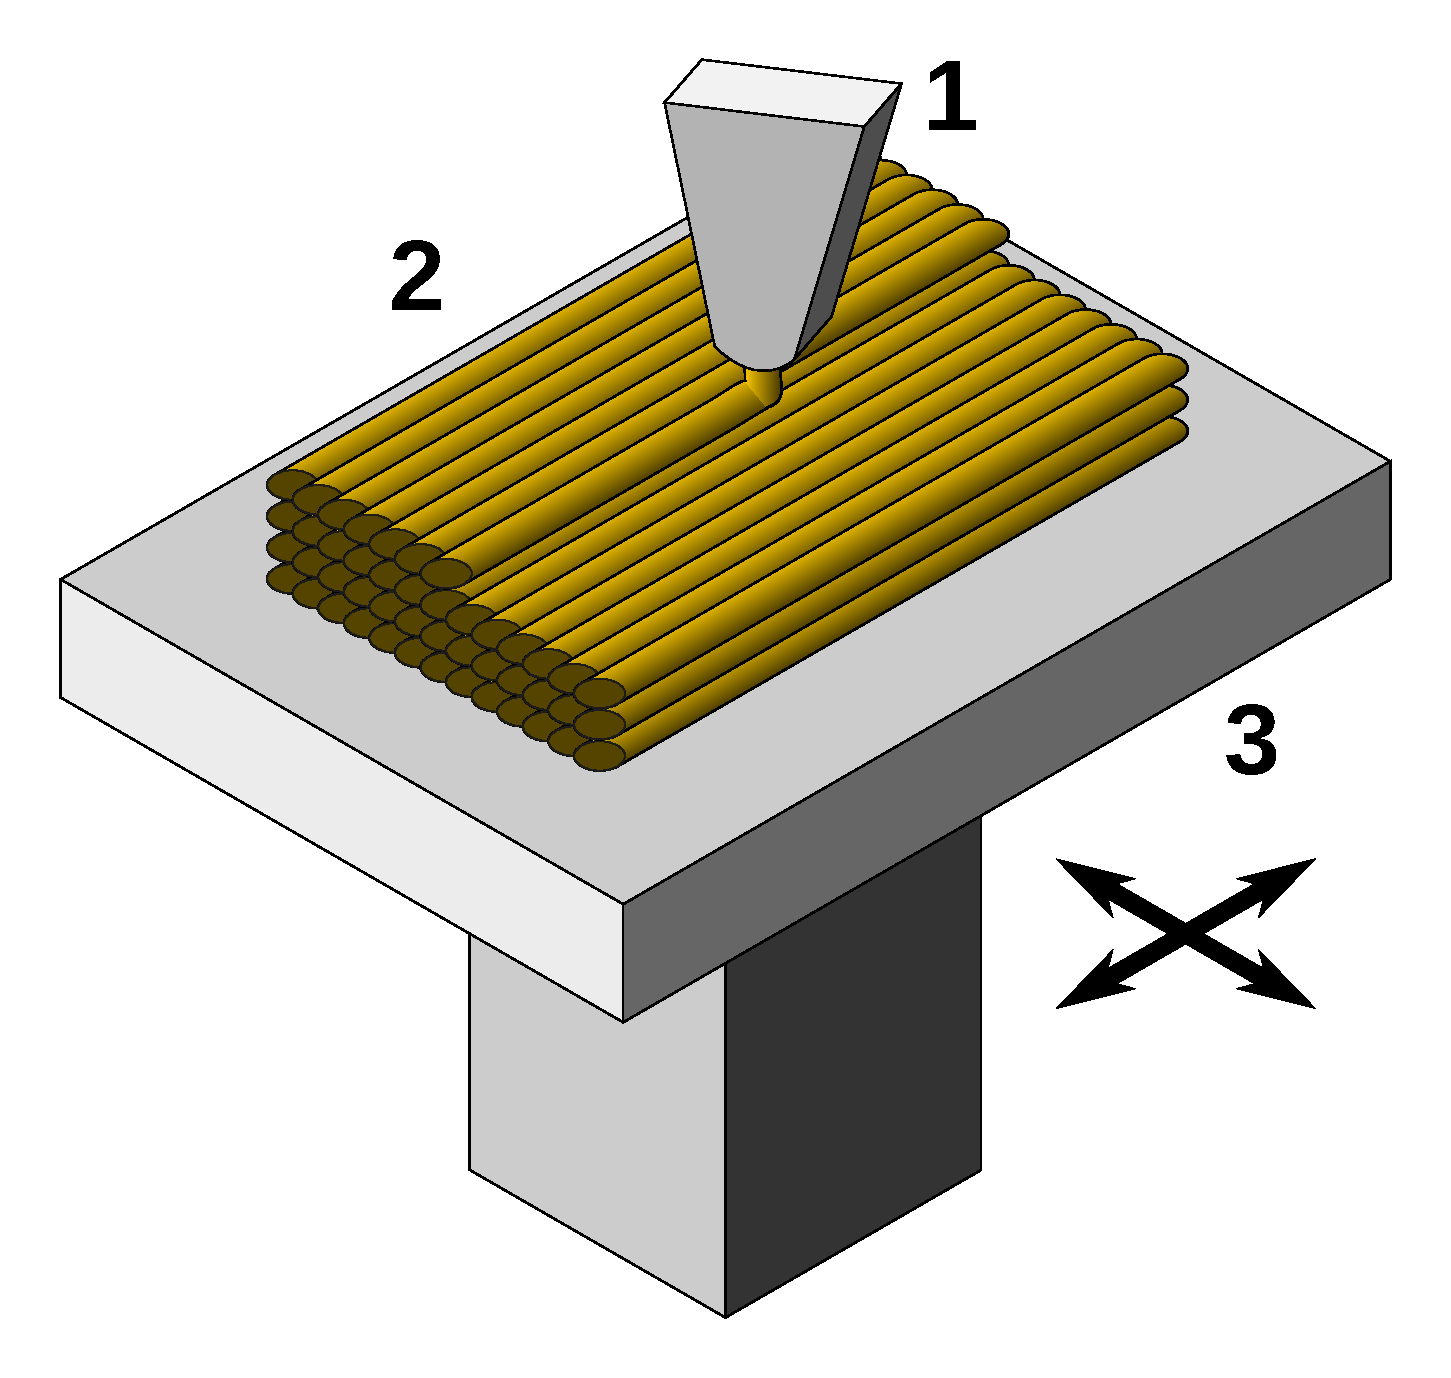
\includegraphics[width=7cm]{Images/4/FDM_printing.pdf}
		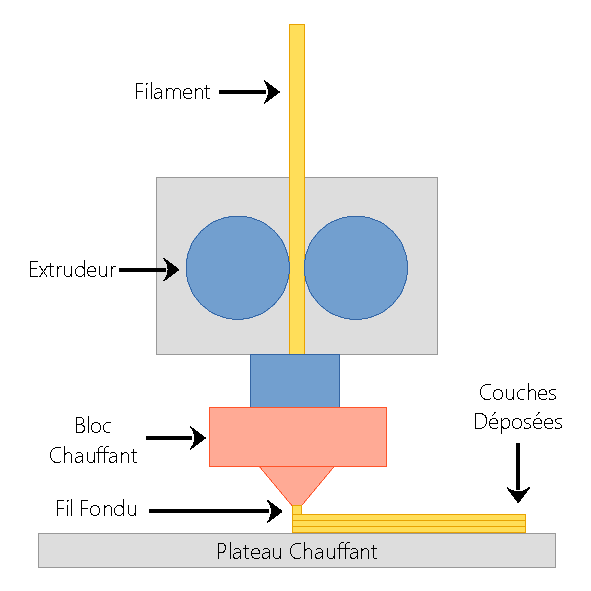
\includegraphics[width=7cm]{Images/4/impression_3D_schema.pdf}
		\caption{Principe de fonctionnement de la technologie d’impression 3D type FDM \cite{principe_fdm}}
	\end{figure}
	
	Cette technologie utilise un filament d’un diamètre calibré. Ce filament est poussé par un extrudeur dans un corps chauffant afin de le faire fondre. Le fil fondu sort alors d’une buse d’un diamètre calibré inférieur au diamètre du filament pour être déposé sur un plateau. Le mouvement de l’ensemble extrudeur et bloc chauffant correctement coordonné avec le flux de filament imposé par l’extrudeur forme des motifs. La pièce est alors imprimée par superposition de couches. Nous avons choisi cette méthode de fabrication additive, car c’est une technologie simple, peu chère et nous possédons trois machines de ce type.\\
	
	À partir d’une technologie de ce type il est très simple de produire des pièces à formes très complexes dans les trois dimensions, dont les structures lattices.
	\newpage
	
	\subsubsection{Paramètres du Slicer}
	\hspace{0.5cm}Les paramétrages du slicer ne sont pas à négliger. En effet, étant donné que nous imprimons des motifs extrêmement fins (de l'ordre de $0.2 mm$), ceci implique de devoir faire des réglages très fins. Le slicer utilisé tout au long du projet est le logiciel \textit{Prusa Slicer} basé sur le slicer \textit{Slic3r}. Nous avons choisi ce logiciel car il nous laisse une grande liberté dans le choix des paramètres d'impression. Il est également très bien documenté ce qui facilite le paramétrage (\href{https://help.prusa3d.com/fr/category/prusaslicer_204}{Lien vers la documentation de \textit{Prusa Slicer}}).\\
	
	\textbf{Attention ! : Les paramètres ci-dessous ont été optimisés pour des machines du type Creality Ender-3, Creality CR-10, Creality Ender-3, Alfawise U20, etc... et sont susceptibles de ne pas fonctionner sur d'autres machines.}\\
	
	\underline{Paramètres de l'imprimante :}\\
	
	La première chose à faire est de paramétrer le diamètre de la buse. Dans la majorité des cas, les épaisseurs de parois des structures nous contraignaient à effectuer les impressions avec une buse de $0.2 mm$. Plus le diamètre de buse est faible, plus la longueur de rétractation\footnote{La rétractation est le fait de retirer légèrement le filament de la buse lors des déplacements afin d'éviter la formation de cheveux d'ange.} à besoin d'être faible. Attention à ne pas trop augmenter la longueur de rétractation et attention à ne pas effectuer trop de rétractations ! Cela pourrait boucher la buse. Pour éviter ce problème nous avons paramétrer la longueur de rétractation à $2 mm$ à une vitesse de rétractation de $80 mm/s$, une vitesse de réinsertion de $50 mm/s$ et un déplacement minimal après rétractation de $10 mm$.
	
	\begin{table}[h]
		\centering
		\begin{tabular}{|c|c|}
			\hline
			\rowcolor{Gray}
			\textbf{Nom de la Variable} & \textbf{Valeur}\\
			\hline\hline
			nozzle\_diameter[0] & $0.2 mm$\\
			min\_layer\_height[0] & $0.05 mm$\\
			max\_layer\_height[0] & $0.2 mm$\\
			retract\_lift[0] & $0.4 mm$\\
			retract\_length[0] & $2 mm$\\
			retract\_speed[0] & $80 mm/s$\\
			deretract\_speed[0] & $60 mm/s$\\
			\hline
		\end{tabular}
		\caption{Paramètres de l'imprimante dans \textit{Prusa Slicer}}
	\end{table}

	\underline{Paramètres du filament :}\\
	
	Afin de rendre nos structures les plus homogènes possibles, il est obligatoire que les couches d'impression et les passages successifs de buse dans une même couche donne un solide le plus fusionné (homogène) possible. Cependant, il ne faut pas non plus surchauffer le filament. Cela pourrait casser les chaînes du polymère, engendrant de grands changements de propriétés mécanique. De plus, surchauffer le filament le rends moins visqueux et le risque de former des cheveux d'anges augmente. Nous avons alors décidé de paramétrer la température d'extrusion à $220 ^{\circ} C$, la température du plateau chauffant à $60 ^{\circ} C$ (afin de faciliter l'adhésion de la première couche au plateau). Nous avons également désactivé les ventilateurs de refroidissement du filament pour éviter qu'un fil déposé ne refroidisse trop vite et faciliter la fusion de plusieurs passages de buse. Cela permet également de prévenir des déformations dues au refroidissement.
	
	\begin{table}[h]
		\centering
		\begin{tabular}{|c|c|}
			\hline
			\rowcolor{Gray}
			\textbf{Nom de la Variable} & \textbf{Valeur}\\
			\hline\hline
			filament\_diameter & $1.75 mm$\\
			filament\_density & $1.24 g/cm^{3}$\\
			first\_layer\_temperature & $220 ^{\circ} C$\\
			temperature & $220 ^{\circ} C$\\
			first\_layer\_bed\_temperature & $60 ^{\circ} C$\\
			bed\_temperature & $60 ^{\circ} C$\\
			fan\_always\_on & False\\
			cooling & False\\
			bridge\_fan\_speed & $100 \%$\\
			\hline
		\end{tabular}
		\caption{Paramètres du filament dans \textit{Prusa Slicer}}
	\end{table}
	\newpage
	
	\underline{Paramètres d'impression :}\\
	
	\hspace{0.5cm}Nous avons expliqué précédemment que la température d'extrusion du filament est importante pour obtenir une bonne fusion des couches entre-elles. Ce paramètre n'est pas le seul influent sur la fusion des couches. En effet, si la température est très élevée mais qu'il y a une hauteur de $0.5 mm$ entre les couches, l'effet de la température n'aura quasiment aucun impact. Afin d'avoir un bon compromis entre temps d'impression et qualité de la fusion entre couches, nous avons choisi une hauteur de couche de $0.15 mm$. De manière générale, la hauteur de couche ne doit pas dépasser $80 \%$ du diamètre de la buse.\\
	
	Nos structures ont des parois fines. Cela peut les rendre difficiles à reconnaître par le slicer. Pour se faire nous lui indiquons qu'il doit effectuer un périmètre supplémentaire si nécessaire et nous paramétrons la largeur d'extrusion à $0.151 mm$. Pratiquement la largeur d'extrusion ne peut pas être inférieure à la hauteur de couche, nous la paramétrons au plus bas afin d'imprimer les épaisseurs les plus fines.\\
	
	Nous avons remarqué que dans le cas de structures n'ayant qu'un seul passage de buse pour l'épaisseur de la paroi, les losanges pouvaient ne pas être soudés entre eux dans certains cas. En vérifiant la configuration, nous nous sommes aperçus que le générateur de périmètre "Classique" engendrait ce phénomène. Il faut donc le paramétrer sur "Arachne".
	
	\begin{figure}[H]
		\centering
		\begin{tabular}{c}
			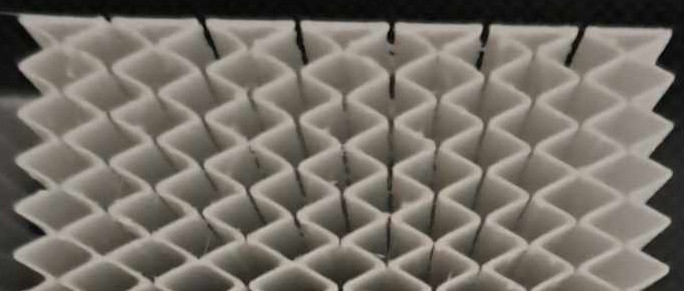
\includegraphics[width=7cm]{Images/4/jointure_murs.jpg}\\
			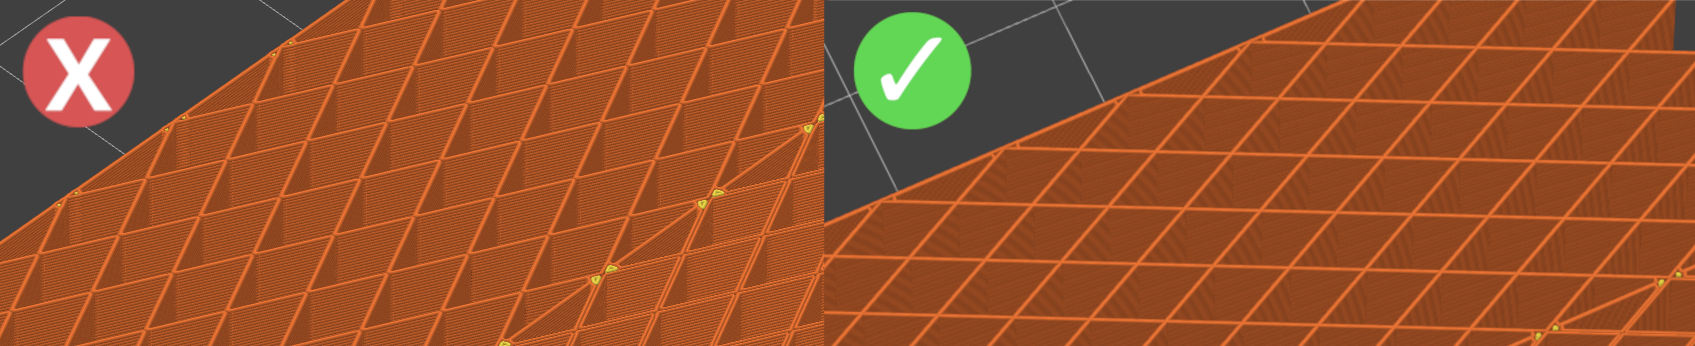
\includegraphics[width=16cm]{Images/4/ok_nok_perimetres.png}\\
		\end{tabular}
		\caption{Problématique de fusion entre losange non réalisée lors de l'impression avec le générateur de périmètres "Classique"}
	\end{figure}

	La vitesse d'impression est cruciale et doit-être abaissée par rapport à des impressions classiques avec une buse de $0.4 mm$ sinon la buse peut se boucher ou l'extrudeur peut grignoter le filament. Nous avons imprimé nos structures à une vitesse de $60 mm/s$.
	
	\begin{table}[h]
		\centering
		\begin{tabular}{|c|c|}
			\hline
			\rowcolor{Gray}
			\textbf{Nom de la Variable} & \textbf{Valeur}\\
			\hline\hline
			layer\_height & $0.15 mm$\\
			first\_layer\_height & $0.15 mm$\\
			extra\_perimeters & True\\
			gap\_fill\_enabled & True\\
			perimeter\_generator & Arachne\\
			fill\_density & $100 \%$\\
			fill\_pattern & Rectilinear\\
			perimeter\_speed & $60 mm/s$\\
			small\_perimeter\_speed & $60 mm/s$\\
			extarnal\_perimeter\_speed & $60 mm/s$\\
			\hline
		\end{tabular}
		\begin{tabular}{|c|c|}
			\hline
			\rowcolor{Gray}
			\textbf{Nom de la Variable} & \textbf{Valeur}\\
			\hline\hline
			infill\_speed & $60 mm/s$\\
			solid\_infill\_speed & $60 mm/s$\\
			extrusion\_width & $0.151 mm$\\
			first\_layer\_extrusion\_width & $0.151 mm$\\
			perimeter\_extrusion\_width & $0.151 mm$\\
			infill\_extrusion\_width & $0.151 mm$\\
			solid\_infill\_extrusion\_width & $0.151 mm$\\
			top\_infill\_extrusion\_width & $0.151 mm$\\
			infill\_overlap & $50 \%$\\
			\hline
		\end{tabular}
		\caption{Paramètres d'impression dans \textit{Prusa Slicer}}
	\end{table}
	
	\newpage
	
	\section{Structures Développées}
	\subsection{Structure N°1 : Losanges}
	\label{losanges}
	\hspace{0.5cm}La première structure que nous avons développée est une structure de base, que l’on peut retrouver dans les slicer d’impression 3D par exemple. Dans le but de générer cette structure, nous avons définit les paramètres suivants :
	
	\begin{figure}[H]
		\centering
		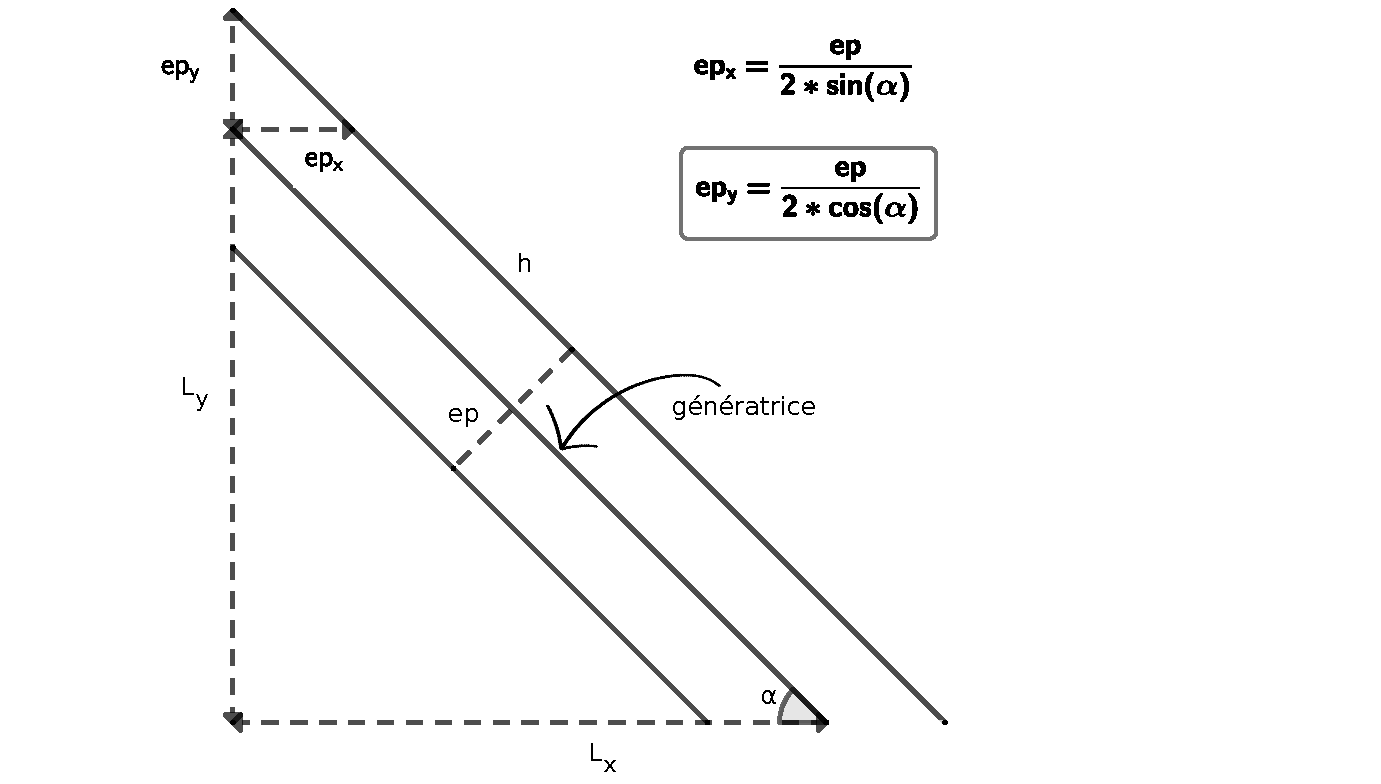
\includegraphics[width=10cm]{Images/5/losanges.pdf}
		\caption{Paramètres de la géométrie N°1 : Losanges}
	\end{figure}
	
	Un losange possédant deux axes de symétrie, nous n’avons représenté qu’un quart de la géométrie sur la figure ci-dessus. Afin de générer un losange entier, il nous suffisait de répéter cette forme quatre fois en appliquant une symétrie centrale. Un losange complet est donc de dimensions $(2* L_x)*(2*L_y).$
	
	\begin{table}[h]
		\centering
		\begin{tabular}{|c|c|c|}
			\hline
			\rowcolor{Gray}
			\textbf{Nom} & \textbf{Variable} & \textbf{Description} \\
			\hline\hline
			$ep$ & Epaisseur des parois & Paramètre d'entrée \\
			$\alpha$ & Angle des losanges & Paramètre d'entrée \\
			$L_x$ & Largeur du motif à répéter & Paramètre calculé \\
			$L_y$ & Hauteur du motif à répéter & Paramètre calculé \\
			$ep_x$ & Epaisseur de paroi projetée sur $\vec{x}$ & Paramètre calculé \\
			$ep_y$ & Epaisseur de paroi projetée sur $\vec{y}$ & Paramètre calculé \\
			\hline
		\end{tabular}
		\caption{Paramètres de la géométrie N°1 : Losanges}
	\end{table}
	
	\underline{Voici un aperçu d'une structure losange de référence, modélisée sous \textit{FreeCAD} à l’aide des paramètres}\\
	\underline{prédéfinis :}
	
	\begin{figure}[H]
		\centering
		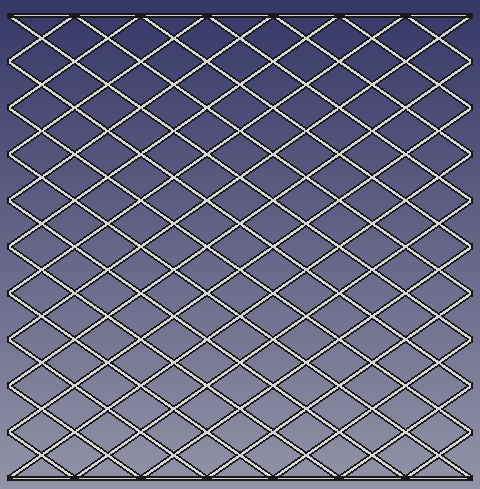
\includegraphics[width=5cm]{Images/5/Freecad_losanges.png}
		\caption{Modélisation sous \textit{FreeCAD} d’une structure N°1 : Losanges}
	\end{figure}
	
	Pour générer cela, nous commençons par générer un losange que nous répétons suivant l’axe $\vec{x}$, puis nous répétons la ligne entière suivant $\vec{y}$ jusqu’en haut de la structure.
	\newpage
	
	\subsection{Structure N°2 : Triangles}
	\hspace{0.5cm}La deuxième structure que nous avons développée est une structure à base de triangles. Ces triangles sont tous isocèles et les épaisseurs sont constantes entre tous les triangles.
	
	\begin{figure}[H]
		\centering
		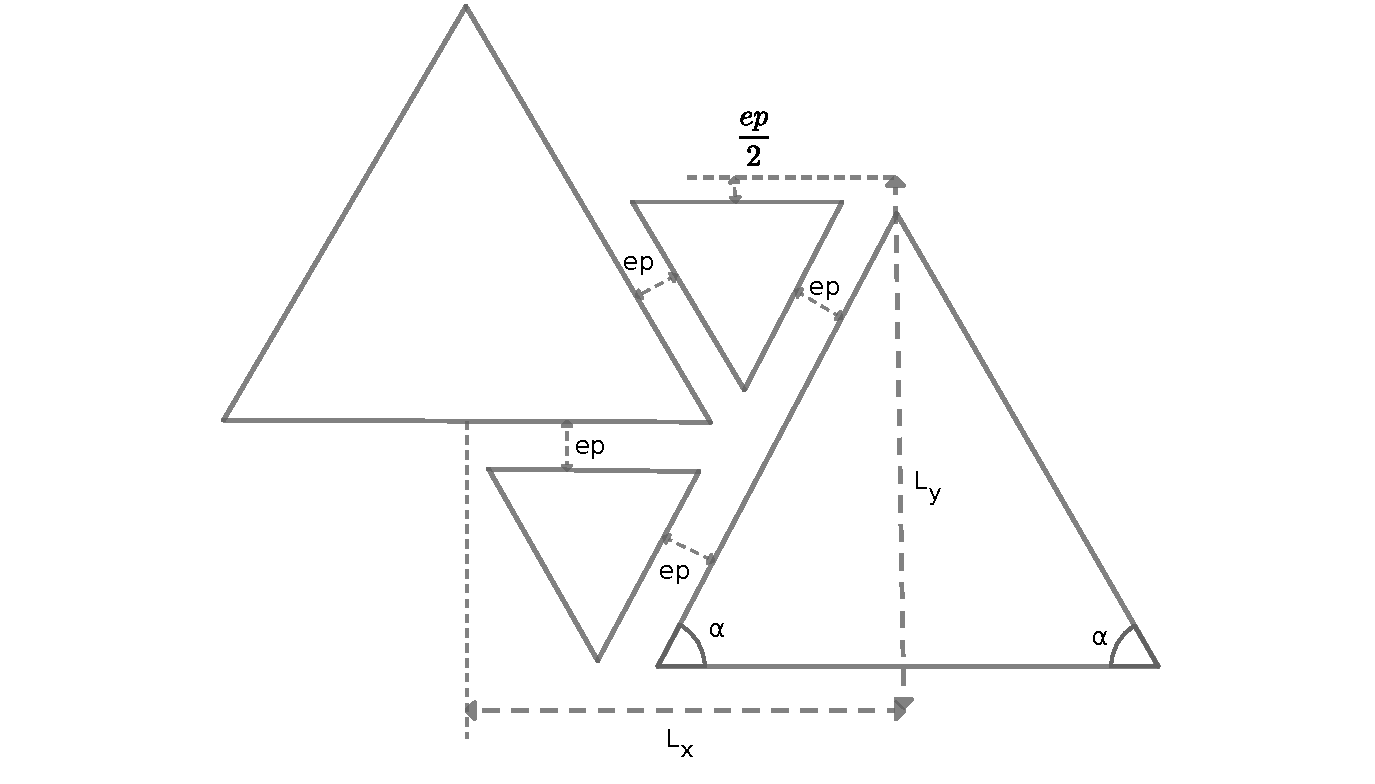
\includegraphics[width=9cm]{Images/5/triangle_1.pdf}
		\caption{Paramètres de la géométrie N°2 : Triangles}
	\end{figure}
	
	\underline{Voici les paramètres de cette structure :}
	
	\begin{table}[H]
		\centering
		\begin{tabular}{|c|c|c|}
			\hline
			\rowcolor{Gray}
			\textbf{Nom} & \textbf{Variable} & \textbf{Description} \\
			\hline\hline
			$ep$ & Epaisseur des parois & Paramètre d'entrée \\
			$\alpha$ & Angle du triangle & Paramètre d'entrée \\
			$L_x$ & Largeur du motif à répéter & Paramètre calculé \\
			$L_y$ & Hauteur du motif à répéter & Paramètre calculé \\
			\hline
		\end{tabular}
		\caption{Paramètres de la géométrie N°2 : Triangles}
	\end{table}
	
	\underline{Notre structure possédant des axes de symétrie, nous avons décidé de la réduire à cette géométrie suivante,}\\
	\underline{afin de simplifier la modélisation :}
	
	\begin{figure}[H]
		\centering
		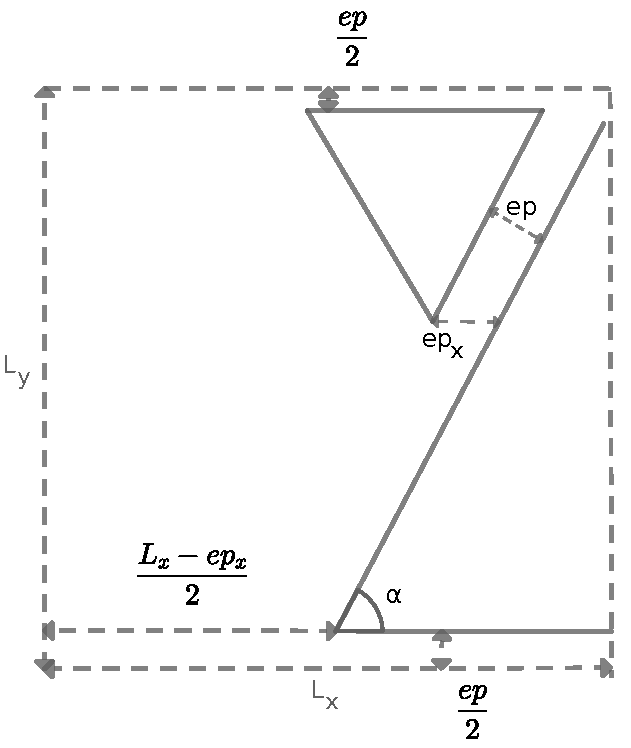
\includegraphics[height=7.5cm]{Images/5/triangle_2.pdf}
		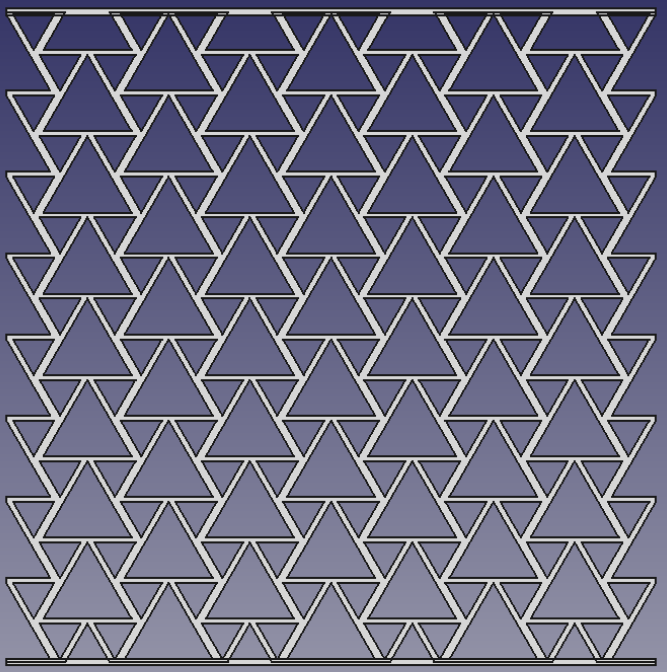
\includegraphics[height=7.5cm]{Images/5/Freecad_triangles.png}
		\caption{Motif à répéter de la géométrie N°2 : Triangles à gauche. Modélisation sous \textit{FreeCAD} d’une structure N°2 : Triangles à droite.}
	\end{figure}
	
	Nous avons répété ce motif tous les $L_x$ suivant $\vec{x}$ et tous les $\frac{L_y}{2}$ suivant $\vec{y}$ afin de générer la structure dans son ensemble. Voici une représentation de la structure triangle modélisée sous \textit{FreeCAD}.
	\newpage
	
	\subsection{Structure N°3 : Carrés + Arc}
	\hspace{0.5cm}La quatrième structure que nous avons développée est une structure à base d’arcs de cercles et de carrés. Ces derniers sont tous de même dimensions tout en gardant une épaisseur de parois constante. Pour sa génération nous avons développé un motif (présenté ci dessous) auquel nous appliquerons la symétrie pour obtenir la structure finale.
	
	\begin{figure}[H]
		\centering
		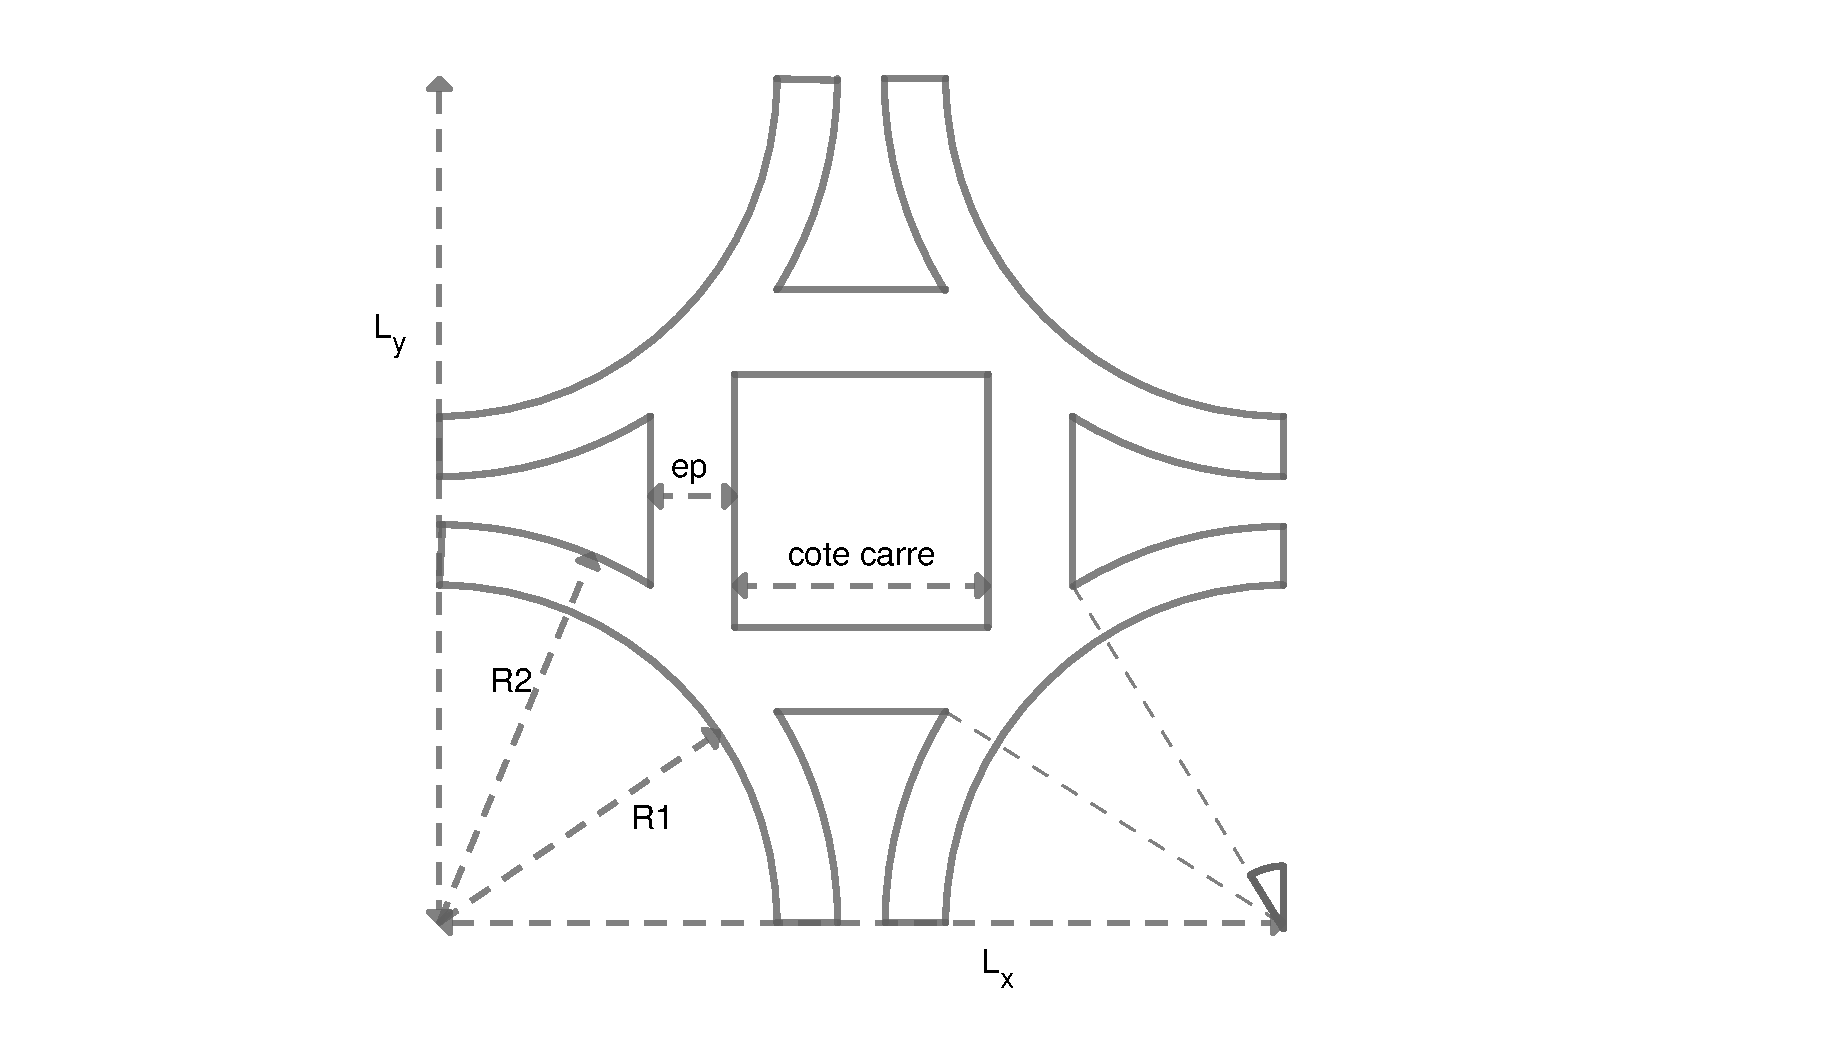
\includegraphics[width=11cm]{Images/5/carres+arc_2D.pdf}
		\caption{Paramètres de la géométrie N°3 : Carrés + Arcs}
		\label{struct_no3}
	\end{figure}
	
	\begin{table}[H]
		\centering
		\begin{tabular}{|c|c|c|}
			\hline
			\rowcolor{Gray}
			\textbf{Nom} & \textbf{Variable} & \textbf{Description} \\
			\hline\hline
			$ep$ & Epaisseur des parois & Paramètre d'entrée \\
			$\alpha$ & Angle délimitant le tracé des petits arcs de cercle & Paramètre d'entrée \\
			$L_x$ & Largeur du motif à répéter & Paramètre calculé \\
			$L_y$ & Hauteur du motif à répéter & Paramètre calculé \\
			$R_1$ & Rayon intérieur du cercle & Paramètre calculé \\
			$R_2$ & Rayon extérieur du cercle & Paramètre calculé \\
			\hline
		\end{tabular}
		\caption{Paramètres de la géométrie N°3 : Carrés + Arc}
	\end{table}
	
	De la même manière que précédemment, le motif de la figure \ref{struct_no3} à été répété suivant l’axe $\vec{x}$ puis suivant l’axe $\vec{y}$ afin de former une structure finale que voici :
	
	\begin{figure}[H]
		\centering
		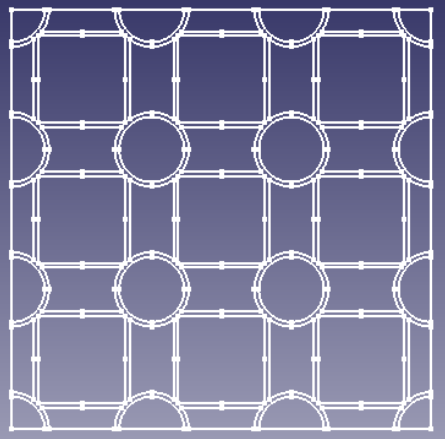
\includegraphics[width=7cm]{Images/5/Freecad_carres.png}
		\caption{Modélisation sous \textit{FreeCAD} d’une structure N°3 : Carrés + Arcs}
	\end{figure}
	\newpage
	
	\subsection{Structure N°4 : Hexagones + Triangles}
	\hspace{0.5cm}Pour cette quatrième structure, nous avons voulu nous inspirer des structures en nid d’abeille, bien connues des slicers d’impression 3D et des structures lattices. Cette structure se compose d’hexagones mis côte à côte complétés par des triangles.\\
	
	\begin{figure}[H]
		\centering
		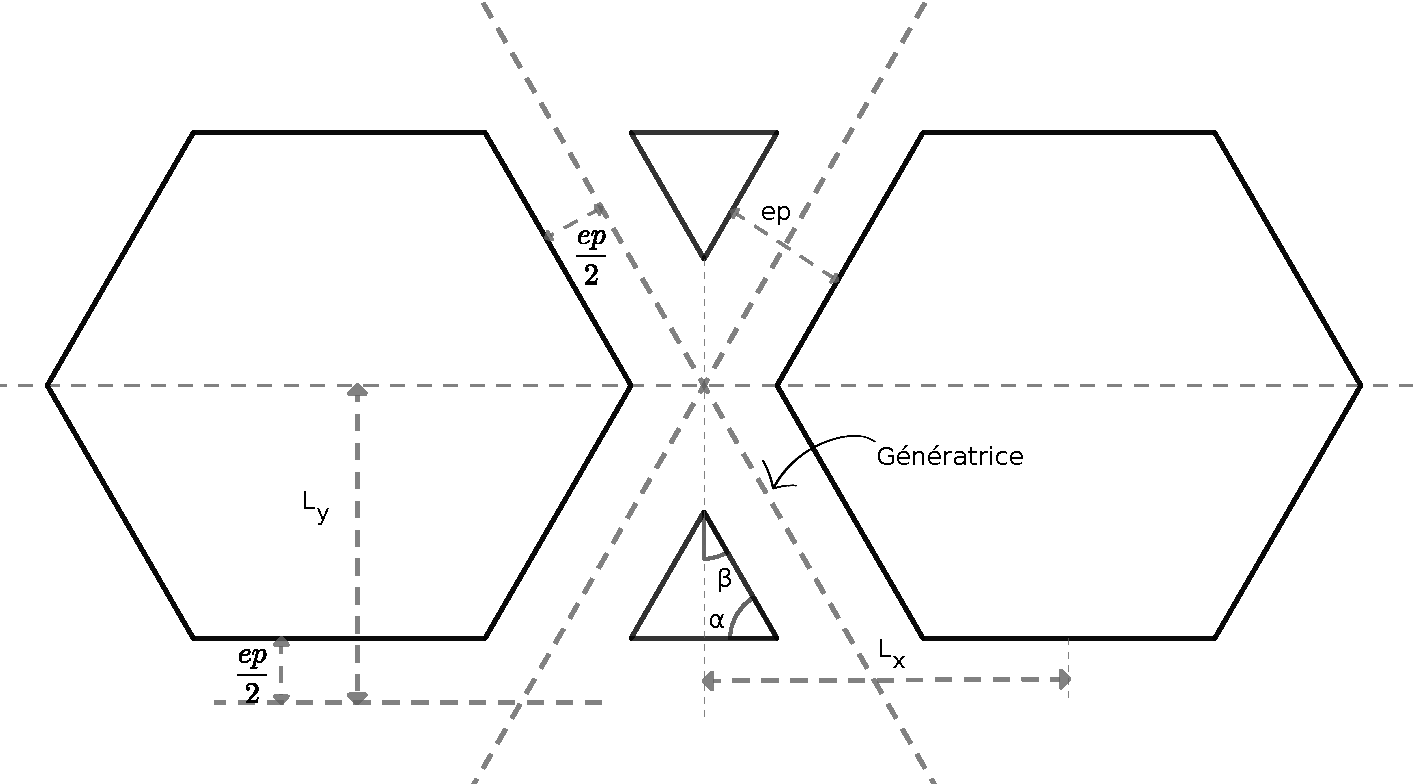
\includegraphics[width=11cm]{Images/5/hexagone.pdf}\\
		\caption{Paramètres de la géométrie N°4 : Hexagones + Triangles}
	\end{figure}
	
	\begin{table}[h]
		\centering
		\begin{tabular}{|c|c|c|}
			\hline
			\rowcolor{Gray}
			\textbf{Nom} & \textbf{Variable} & \textbf{Description} \\
			\hline\hline 
			$ep$ & Epaisseur des parois & Paramètre d'entrée \\
			$\alpha$ & Angle des losanges & Paramètre d'entrée \\
			$L_x$ & Largeur du motif à répéter & Paramètre calculé \\
			$L_y$ & Hauteur du motif à répéter & Paramètre calculé \\
			$ep_x$ & Epaisseur de paroi projetée sur $\vec{x}$ & Paramètre calculé \\
			$ep_y$ & Epaisseur de paroi projetée sur $\vec{y}$ & Paramètre calculé \\
			\hline
		\end{tabular}
		\caption{Paramètres de la géométrie N°4 : Hexagones + Triangles}
	\end{table}
	
	Il existe deux cas de figure pour cette géométrie. En effet, il est possible d’obtenir une structure où les hexagones sont alignés ou déphasés suivant $\vec{y}$.
	
	\begin{figure}[H]
		\centering
		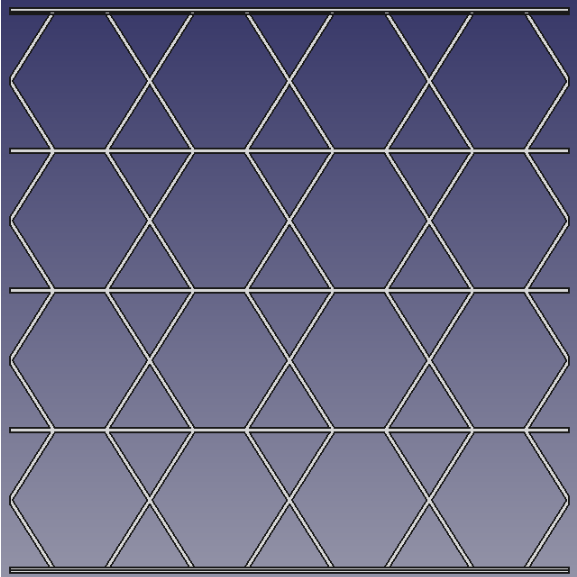
\includegraphics[width=6cm]{Images/5/Freecad_hexagones_alignes.png}
		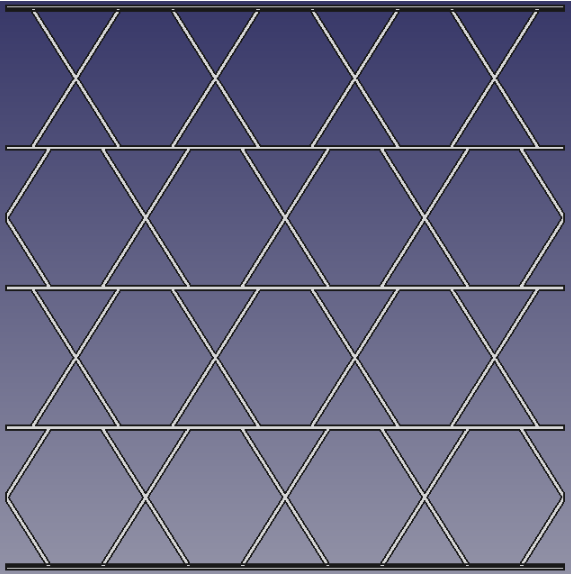
\includegraphics[width=6cm]{Images/5/Freecad_hexagones_dephases.png}
		\caption{Modélisation sous \textit{FreeCAD} d’une structure N°4 : Hexagones + Triangles Alignées à gauche. Modélisation sous \textit{FreeCAD} d’une structure N°4 : Hexagones + Triangles Déphasés à droite.}
	\end{figure}
	\newpage
	
	\subsection{Structure N°5 : Cosinus}
	\hspace{0.5cm}Lors de nos recherches bibliographiques, nous avons observé que de nombreuses structures lattices avaient la forme d’une gyroïde. Cependant la gyroïde est une structure utilisant une fonction mathématique à trois dimensions (3D). N’étudiant uniquement des structures 2D ($y=f(x)$), nous avons choisi d’utiliser une fonction cosinus pour essayer de reproduire l’effet d’une gyroïde en 1D. En effet, l'équation d'une gyroïde se définit comme suit :
	
	\begin{center} 
	{$\sin x\cos y+\sin y\cos z+\sin z\cos x=0$}
	\end{center}
	{ce qui se traduit, lorsque $y=z=0$, par}
	\begin{center}
	{$\sin x=0$}
	\end{center}
	
	En s’inspirant de cela ($f(x)=\sin(x))$, nous avons développé une structure en forme de cosinus (déphasé de $\frac{\pi}{2})$ suivant l’axe $\vec{y}$. Afin de rigidifier la structure, nous avons inséré des plateaux à intervalle réguliers sur l’axe $\vec{x}$.
	
	\begin{figure}[H]
		\centering
		\begin{tabular}{m{6cm}m{5.5cm}}
			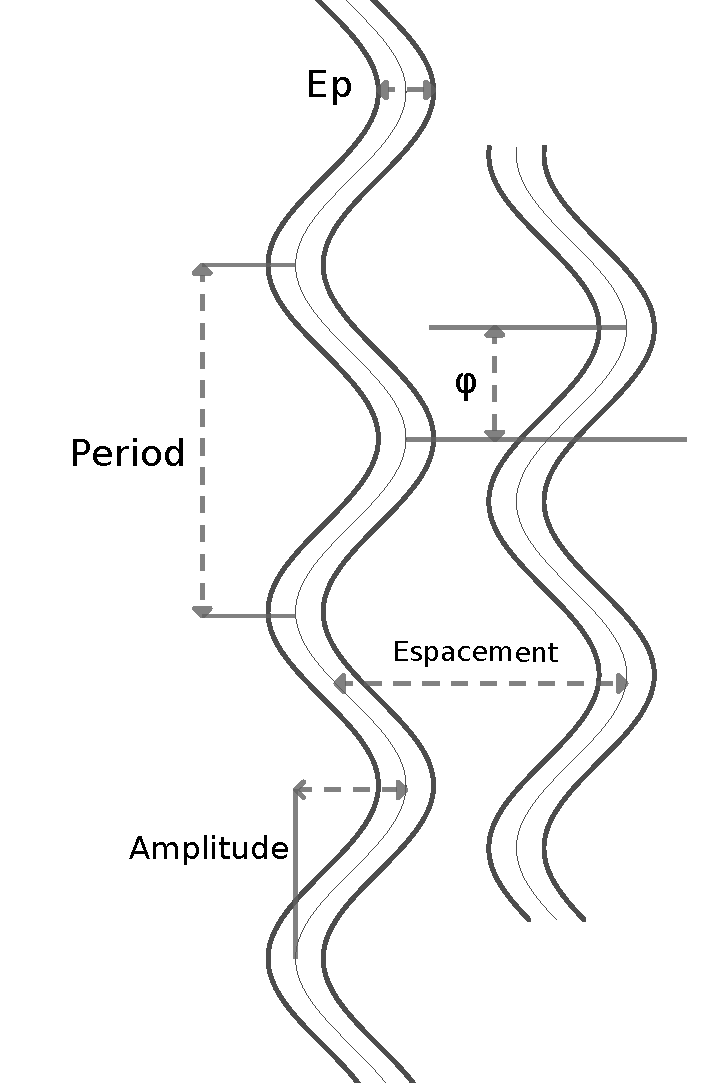
\includegraphics[width=4.5cm]{Images/5/Cosinus.pdf} & 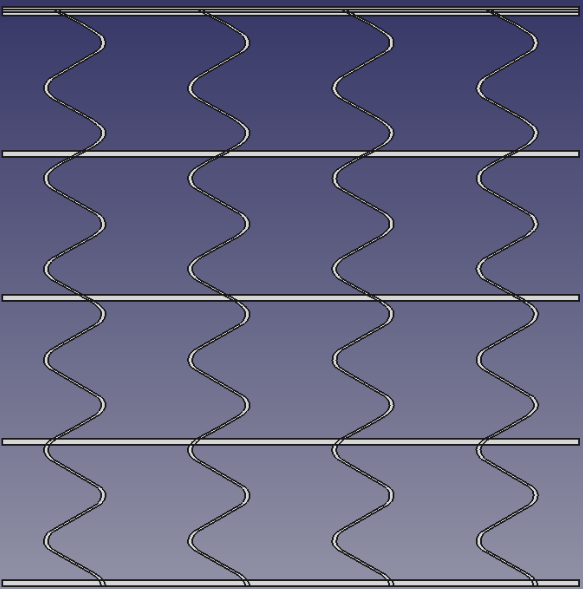
\includegraphics[width=5.5cm]{Images/5/Freecad_cosinus.png}\\
		\end{tabular}
		\caption{Paramètres de la géométrie N°5 : Cosinus à gauche. Modélisation sous \textit{FreeCAD} d’une structure N°5 : Cosinus à droite.}
	\end{figure}	
	
	\begin{table}[H]
		\centering
		\begin{tabular}{|c|c|c|}
			\hline
			\rowcolor{Gray}
			\textbf{Nom} & \textbf{Variable} & \textbf{Description} \\
			\hline\hline 
			$ep$ & Epaisseur des parois & Paramètre d'entrée \\
			$\phi$ & Déphasage entre les différentes couches du cosinus & Paramètre d'entrée \\
			Period & Période du cosinus & Paramètre d'entrée \\
			Espacement & Espacement entre deux couches du cosinus & Paramètre d'entrée \\
			Amplitude & Amplitude du cosinus & Paramètre d'entrée \\
			\hline
		\end{tabular}
		\caption{Paramètres de la géométrie N°5 : Cosinus}
	\end{table}
	
	\hspace{0.5cm}Cette structure n’aurait néanmoins pas produit des résultats très probants si les cosinus s'étendaient sur une distance de 40 mm. En effet, il est très probable que les paroies des cosinus fléchissent violemment sur le côté avant de rompre. Afin de limiter cet effet, nous avons décidé d’ajouter des plateaux liant les cosinus entre eux à intervalle régulier.
	\newpage
	
	\section{Expérimentations}
	\subsection{Matériel utilisé}
	\hspace{0.5cm}Plusieurs systèmes existent afin de réaliser un essai de dynamique rapide. Parmi eux on peut retrouver les essais avec des barres d'Hopkinson, les machines hydrauliques ou encore les lanceurs à gaz. Nous cherchions à faire des essais mécaniques où nous puissions facilement calibrer l'énergie d'impact sur notre structure. Nous voulions également effectuer un maximum d'essais en un temps très court. La solution du Puits de Chute s'est donc imposée.
	
	\begin{figure}[H]
		\centering
		\includegraphics[width=11cm]{Images/6/Puits_de_chute.png}\\
		\caption{Plan technique du Puits de Chute original issu de la thèse de Audrey Auperrin \cite{these_auperrin}}
	\end{figure}
	
	Le principe est simple. Une masse d'impact est lâché d’une hauteur précise sur une structure à étudier. Ceci nous permettra de mesurer la capacité de la structure à absorber l'énergie d'impact. Le puits de chute est composé de :
	
	\begin{itemize}
		\item Une masse coulissante sur les deux axes de guidages verticaux.
		\item Un capteur laser mesurant le déplacement de l'impacteur.
		\item Une cellule de force de $7 kN$ mesurant l'effort subit par la structure lors de l'impact.
	\end{itemize}

	Le Puits de Chute originalement conçu lors de la thèse de Audrey Auperrin \cite{these_auperrin} n'était pas adapté à notre utilisation. Il a donc été nécessaire de modifier le puits de chute en concevant un impacteur ainsi qu'un support pour la cellule de force. Ces pièces ont été usinées en aluminium au LAMIH\footnote{Laboratoire d'Automatique, de Mécanique et d'Informatique Industrielles et Humaines}. Les pièces que nous avons conçues apparaissent en bleu sur la figure \ref{pieces_pdc}.
	
	\begin{figure}[H]
		\centering
		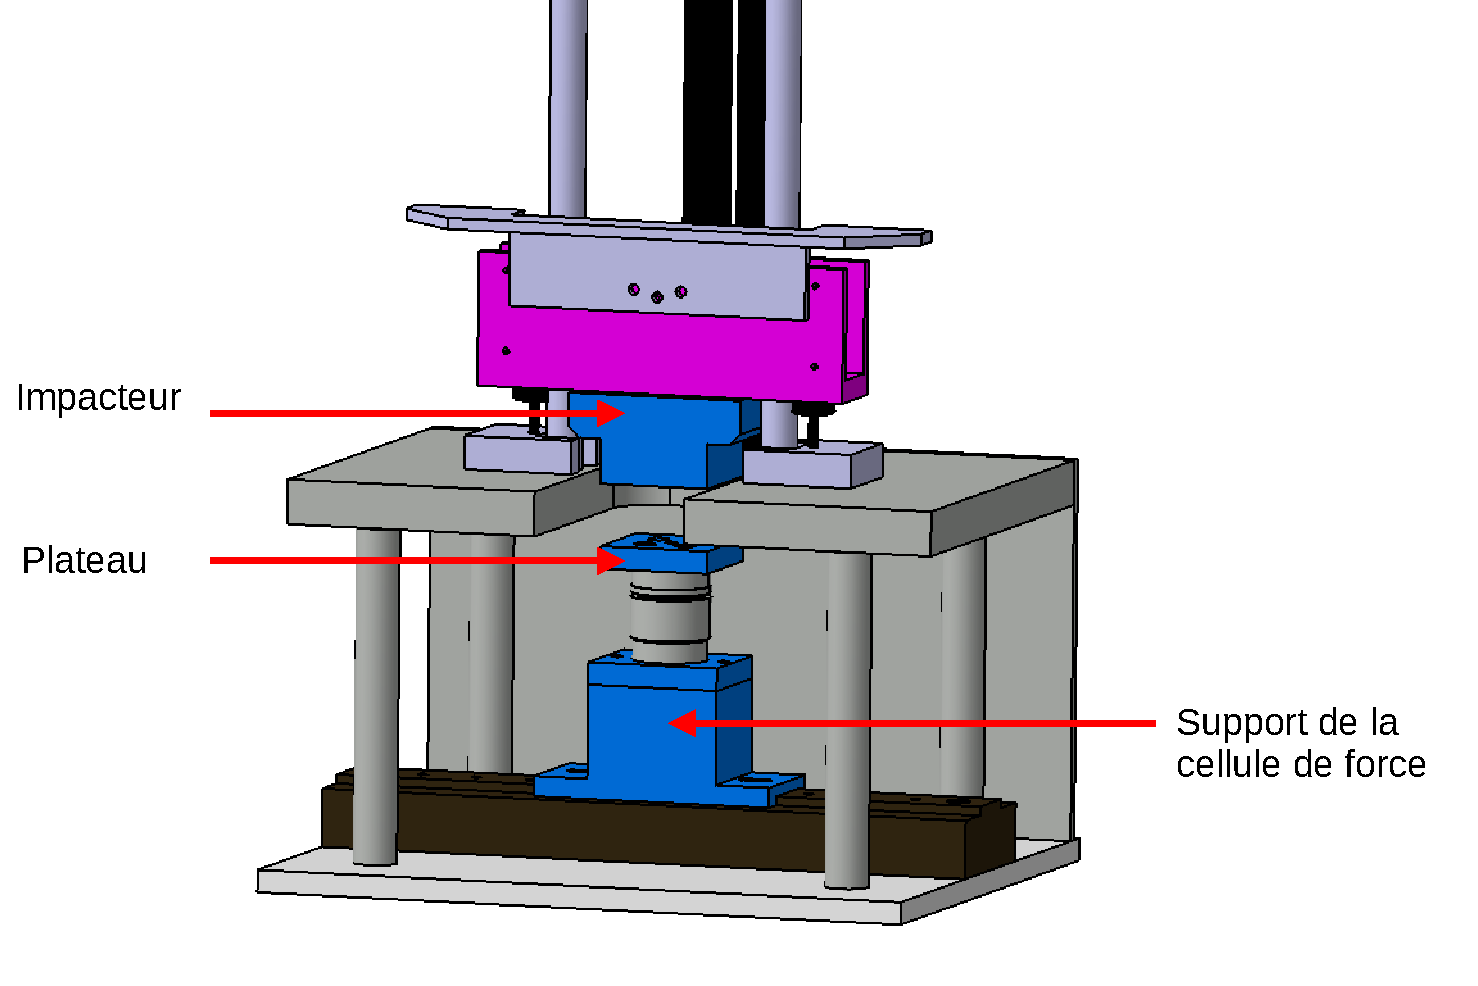
\includegraphics[width=11cm]{Images/6/conception_finale.pdf}\\
		\caption{Schéma des éléments du puits de chute modélisés sous \textit{Catia V5}}
		\label{pieces_pdc}
	\end{figure}
	\newpage
	
	\subsection{Protocole expérimental}	
	\begin{figure}[H]
		\centering
		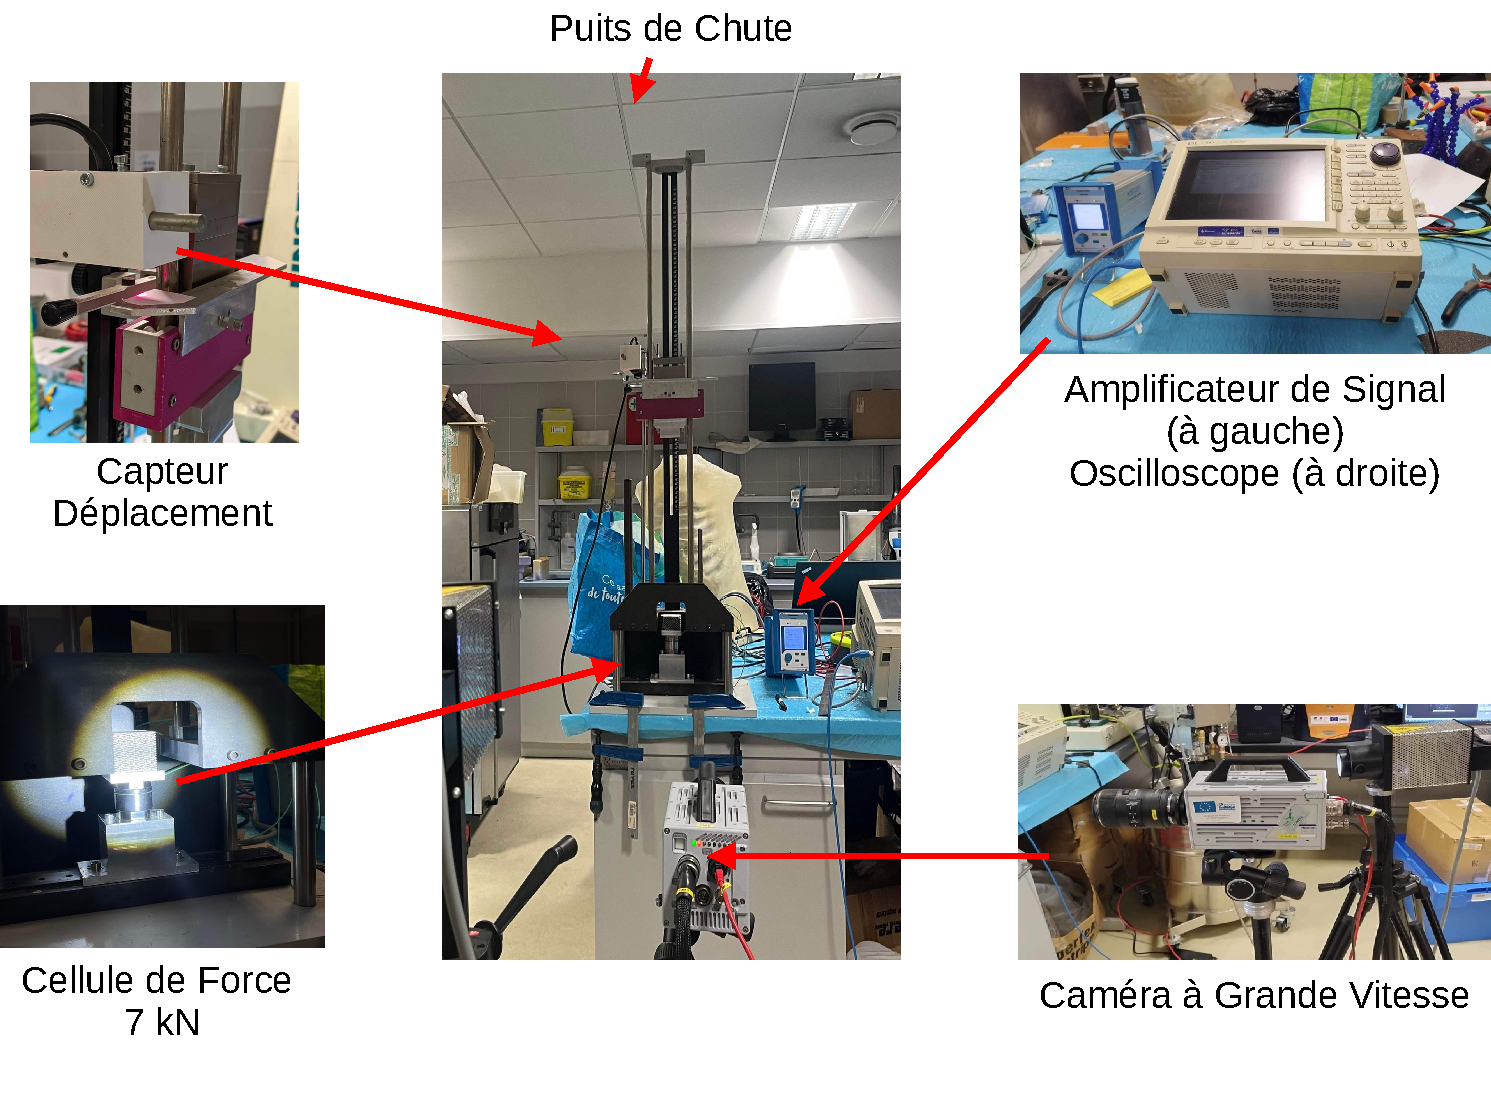
\includegraphics[width=15cm]{Images/6/protocole.pdf}
		\caption{Schéma de l'installation expérimentale}
	\end{figure}

	\hspace{0.5cm}Le protocole expérimental est simple. Une structure est installée sur la cellule de force. Pour éviter que la base de la structure ne glisse lors de l'essai, nous l'avons fixée avec de l'adhésif double face. Une fois la structure installée, il faut impérativement effectuer le tarage de la cellule d'effort. En effet, celle-ci est de type piézoélectrique ce qui lui permet d'effectuer une mesure avec précision sur une large plage mais est extrêmement sensible et nécessite un recalibrage après chaque essais. La caméra à grande vitesse doit ensuite débuter l'enregistrement sans fin (elle effectue un enregistrement jusqu'à ce que l'oscilloscope envoie son signal de trigger). Une fois l'oscilloscope prêt, la masse peut-être lâchée. Vient ensuite la partie d'analyse des données récoltées.\\
	
	Afin d'effectuer nos essais dans les mêmes conditions, nous devons effectuer ces derniers à énergie d'impact constante. Pour cela, nous avons fixé une masse et une hauteur d'impact. La masse d'impact est fixée à $3344,65 g$ et la hauteur d'impact est fixée à $41,8 cm$. Nous avons déterminé ces valeurs en effectuant quelques essais de calibration. Nous avons arrêté d'augmenter l'énergie d'impact lorsque la structure de référence était totalement écrasée.\\
	
	\underline{Calcul de l'énergie potentielle :}\\
	\label{energie_impact}
	\begin{center}
		$E_{p} = mgh$ avec $g = 9,81 m/s^{2}$, on obtient: $E_{p} = 3,34465 * 9,81 * 0,418 = 13,7 J$
	\end{center}

	L'énergie potentielle se transforme entièrement en énergie cinétique lorsqu'elle atteint la structure et correspond donc à notre énergie d'impact.
	\newpage
	
	\subsection{Variables de l'étude}
	\label{variables_etude}
	\hspace{0.5cm}La structure N°1 (Losanges) s'est avérée être la seule structure prometteuse. Faute de temps et de résultats concluants pour les autres géométries, nous n’avons traité uniquement la structure N°1 (Losanges \ref{losanges}).\\
		
	Comme nous l’avons dit précédemment, afin de pouvoir conclure sur l’influence des paramètres de notre étude, il est crucial que nous ne fassions varier uniquement un seul paramètre à la fois. Nous avons alors établi un plan d’étude qui nous permet dans un premier temps de traiter de l’influence de divers paramètres de la géométrie N°1 (Losanges) sur l’absorption d’énergie.\\
	
	\subsubsection{Gradient d'épaisseur : Épaisseur des parois des Losanges}
	\hspace{0.5cm}Dans un premier temps, nous devions nous assurer que l'ajout de gradient permet en effet d'augmenter l'absorption d'énergie lors d'un crash.\\
	
	La première variable que nous avons étudiée est l'épaisseur de la paroi de la structure. Sur la figure \ref{grad_ep}, la structure de gauche est celle de référence et la structure de droite reprends les mêmes paramètres que celle de référence mais avec un gradient d'épaisseur sur la moitié de sa dimension $\vec{y}$.
	
	\begin{table}[H]
		\centering
		\begin{tabular}{|c|c|c|}
			\hline
			\rowcolor{Gray}
			\multicolumn{3}{c}{Structure de Référence}\\\hline
			\rowcolor{Gray}
			Couche de Gradient & Variable & Valeur\\
			\hline\hline
			  & \textcolor[rgb]{0,0.5,0}{Épaisseur des Parois} & \textcolor[rgb]{0,0.5,0}{0.38 mm}\\
			\textcolor[rgb]{0,0.5,0}{1} & \textcolor[rgb]{0,0.5,0}{Nombre de Losanges sur l'axe $\vec{x}$} & \textcolor[rgb]{0,0.5,0}{7}\\
			  & \textcolor[rgb]{0,0.5,0}{Nombre de Losanges sur l'axe $\vec{y}$} & \textcolor[rgb]{0,0.5,0}{14}\\
			\hline
		\end{tabular}
		\caption{Paramètres de la structure Numéro 1 : Structure de référence}
	\end{table}

	\begin{table}[H]
		\centering
		\begin{tabular}{|c|c|c|}
			\hline
			\rowcolor{Gray}
			\multicolumn{3}{c}{Structure de Référence}\\\hline
			\rowcolor{Gray}
			Couche de Gradient & Variable & Valeur\\
			\hline\hline
			& \textcolor[rgb]{1,0,0}{Épaisseur des Parois} & \textcolor[rgb]{1,0,0}{0.19 mm}\\
			\textcolor[rgb]{1,0,0}{2} & \textcolor[rgb]{1,0,0}{Nombre de Losanges sur l'axe $\vec{x}$} & \textcolor[rgb]{1,0,0}{7}\\
			& \textcolor[rgb]{1,0,0}{Nombre de Losanges sur l'axe $\vec{y}$} & \textcolor[rgb]{1,0,0}{7}\\
			\hline
			& \textcolor[rgb]{0,0.5,0}{Épaisseur des Parois} & \textcolor[rgb]{0,0.5,0}{0.38 mm}\\
			\textcolor[rgb]{0,0.5,0}{1} & \textcolor[rgb]{0,0.5,0}{Nombre de Losanges sur l'axe $\vec{x}$} & \textcolor[rgb]{0,0.5,0}{7}\\
			& \textcolor[rgb]{0,0.5,0}{Nombre de Losanges sur l'axe $\vec{y}$} & \textcolor[rgb]{0,0.5,0}{7}\\
			\hline
		\end{tabular}
		\caption{Paramètres de la structure Numéro 15 : Influence de l'ajout d'un gradient d'épaisseur}
	\end{table}
	
	\begin{figure}[H]
		\centering
		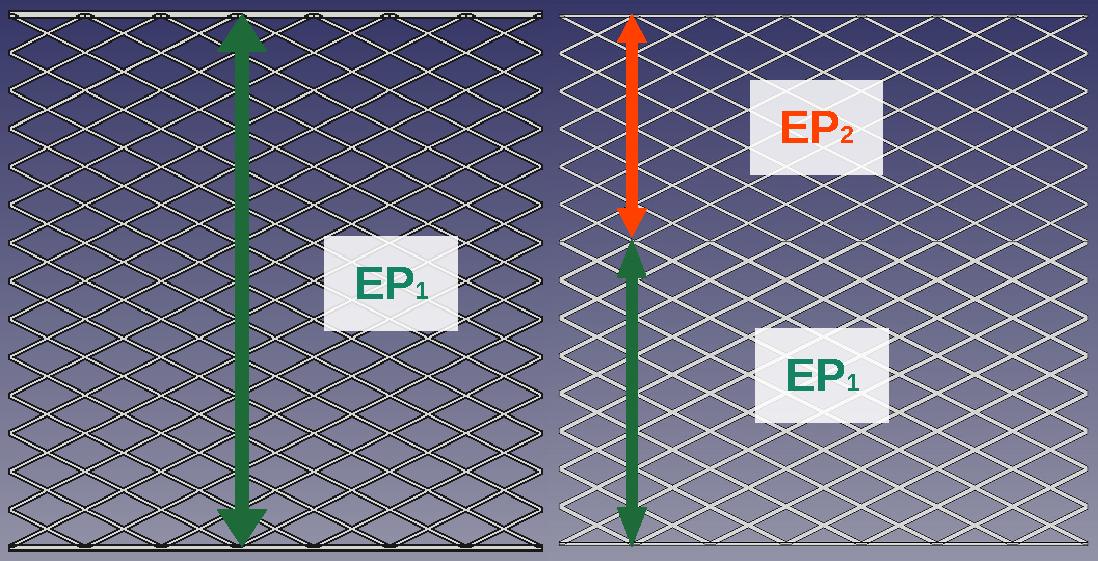
\includegraphics[width=10cm]{Images/6/gradep/gradep.pdf}
		\caption{Étude de l’influence de la présence d'un gradient d'épaisseur au sein d'une structure Losange}
		\label{grad_ep}
	\end{figure}
	\newpage
	
	\subsubsection{Gradient de géométrie : Angle des Losanges}
	\hspace{0.5cm}Nous avons ensuite étudié la variation des angles des Losanges. Pour cela, nous avons réalisé une structure avec un gradient de géométrie mais à épaisseur de parois constante.
	
	%!!!!!!!!!!!!!!!!!!
	\begin{table}[H]
		\centering
		\begin{tabular}{|c|c|c|}
			\hline
			\rowcolor{Gray}
			\multicolumn{3}{c}{Structure de Référence}\\\hline
			\rowcolor{Gray}
			Couche de Gradient & Variable & Valeur\\
			\hline\hline
			& \textcolor[rgb]{0,0.5,0}{Angle des losanges} & \textcolor[rgb]{0,0.5,0}{??? mm}\\
			\textcolor[rgb]{0,0.5,0}{1} & \textcolor[rgb]{0,0.5,0}{Nombre de Losanges sur l'axe $\vec{x}$} & \textcolor[rgb]{0,0.5,0}{???}\\
			& \textcolor[rgb]{0,0.5,0}{Nombre de Losanges sur l'axe $\vec{y}$} & \textcolor[rgb]{0,0.5,0}{???}\\
			\hline
		\end{tabular}
		\caption{Paramètres de la structure Numéro ??? : Structure de référence}
	\end{table}
	
	\begin{table}[H]
		\centering
		\begin{tabular}{|c|c|c|}
			\hline
			\rowcolor{Gray}
			\multicolumn{3}{c}{Structure de Référence}\\\hline
			\rowcolor{Gray}
			Couche de Gradient & Variable & Valeur\\
			\hline\hline
			& \textcolor[rgb]{1,0,0}{Angle des losanges} & \textcolor[rgb]{1,0,0}{??? mm}\\
			\textcolor[rgb]{1,0,0}{2} & \textcolor[rgb]{1,0,0}{Nombre de Losanges sur l'axe $\vec{x}$} & \textcolor[rgb]{1,0,0}{???}\\
			& \textcolor[rgb]{1,0,0}{Nombre de Losanges sur l'axe $\vec{y}$} & \textcolor[rgb]{1,0,0}{???}\\
			\hline
			& \textcolor[rgb]{0,0.5,0}{Angle des losanges} & \textcolor[rgb]{0,0.5,0}{??? mm}\\
			\textcolor[rgb]{0,0.5,0}{1} & \textcolor[rgb]{0,0.5,0}{Nombre de Losanges sur l'axe $\vec{x}$} & \textcolor[rgb]{0,0.5,0}{???}\\
			& \textcolor[rgb]{0,0.5,0}{Nombre de Losanges sur l'axe $\vec{y}$} & \textcolor[rgb]{0,0.5,0}{???}\\
			\hline
		\end{tabular}
		\caption{Paramètres de la structure Numéro ??? : Influence de l'ajout d'un gradient de géométrie}
	\end{table}
	
	\begin{figure}[H]
		\centering
		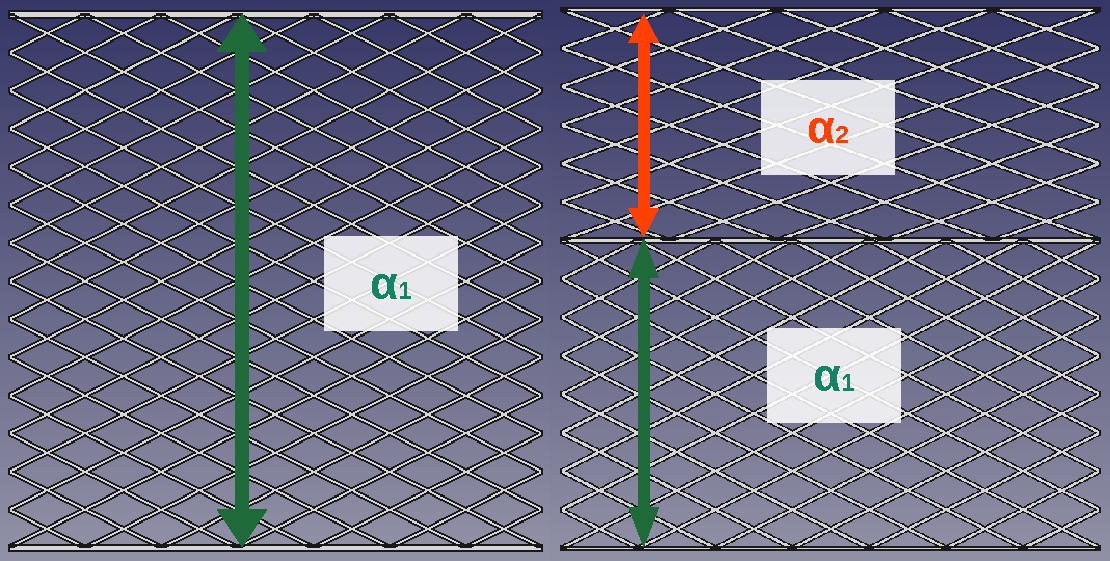
\includegraphics[width=10cm]{Images/6/gradgeom/gradgeom.pdf}\\
		\caption{Étude de l’influence de la présence d'un gradient de géométrie au sein d'une structure losange}
		\label{gradgeom}
	\end{figure}
	\newpage
	
	\subsubsection{Influence de l'ajout de plateaux entre les couches de gradient}
	\hspace{0.5cm}Lorsque nous souhaitons faire varier les angles des losanges en intégrant des gradients de géométrie dans nos structures, nous sommes dans l’obligation d’intégrer des plateaux entre les différentes couches de losanges. En effet, les plateaux entre les couches de gradients de géométrie sont nécessaires afin de lier les deux couches de gradient entre elles.
	
	\begin{figure}[H]
		\centering
		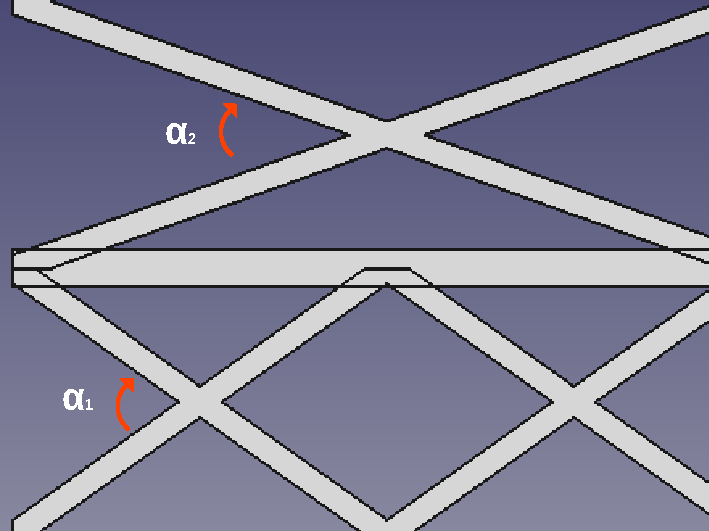
\includegraphics[width=7cm]{Images/6/gradient_geom_alpha.pdf}
		\caption{Représentation de la nécessité d’ajout de plateau dans une configuration de gradient de géométrie}
	\end{figure}

	Puisque nous sommes contraints d'ajouter ces plateaux, il faut que nous étudions leur influence sur l'absorption d'énergie des structures. Pour cela nous avons repris les mêmes paramètres que la structure \textbf{???} \ref{gradgeom} mais avec un gradient d'épaisseur à la place du gradient de géométrie.
	
	%!!!!!!!!!!!!!!!!!!
	\begin{table}[H]
		\centering
		\begin{tabular}{|c|c|c|}
			\hline
			\rowcolor{Gray}
			\multicolumn{3}{c}{Structure de Référence}\\\hline
			\rowcolor{Gray}
			Couche de Gradient & Variable & Valeur\\
			\hline\hline
			& \textcolor[rgb]{1,0,0}{Épaisseur des Parois} & \textcolor[rgb]{1,0,0}{??? mm}\\
			\textcolor[rgb]{1,0,0}{2} & \textcolor[rgb]{1,0,0}{Nombre de Losanges sur l'axe $\vec{x}$} & \textcolor[rgb]{1,0,0}{???}\\
			& \textcolor[rgb]{1,0,0}{Nombre de Losanges sur l'axe $\vec{y}$} & \textcolor[rgb]{1,0,0}{???}\\
			\hline
			& \textcolor[rgb]{0,0.5,0}{Épaisseur des Parois} & \textcolor[rgb]{0,0.5,0}{??? mm}\\
			\textcolor[rgb]{0,0.5,0}{1} & \textcolor[rgb]{0,0.5,0}{Nombre de Losanges sur l'axe $\vec{x}$} & \textcolor[rgb]{0,0.5,0}{???}\\
			& \textcolor[rgb]{0,0.5,0}{Nombre de Losanges sur l'axe $\vec{y}$} & \textcolor[rgb]{0,0.5,0}{???}\\
			\hline
		\end{tabular}
		\caption{Paramètres de la structure Numéro ??? et ??? : Influence de l'ajout d'un plateau entre deux couches}
	\end{table}
	
	\begin{figure}[H]
		\centering
		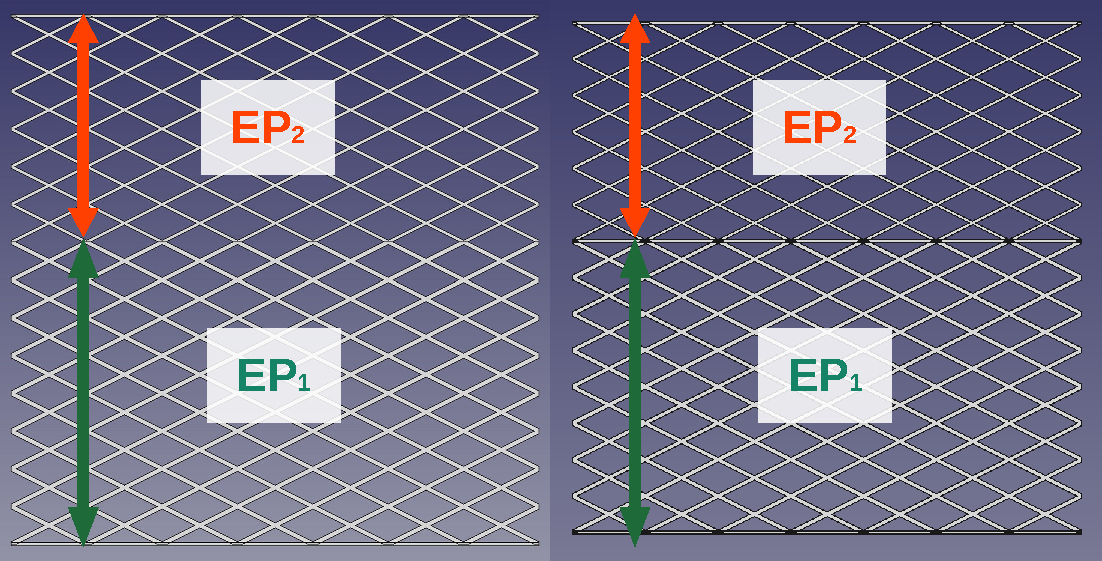
\includegraphics[width=10cm]{Images/6/plateaux/plateaux.pdf}\\
		\caption{ Étude de l’influence de la présence d'un plateau au sein d'une structure losange}
	\end{figure}
	\newpage
	
	\subsubsection{Influence des structures symétriques ou asymétriques}
	\hspace{0.5cm}Les structures asymétriques nous offrent un avantage non négligeable. En effet, lorsque nous voulons intégrer des gradients à nos structures, les gradients asymétriques nous offrent la possibilité d’évoluer sur l’intégralité de la dimension $\vec{y}$ de la structure alors que les structures symétriques ne nous permettent de d’évoluer que sur la moitié de celle-ci. Nous avons donc voulu comparer une structure symétrique avec une structure asymétrique pour mettre en évidence quelle configuration est la plus adaptée pour maximiser l'absorption d'énergie.\\
	
	Pour cela, nous avons comparé une structure B asymétrique, possédant deux couches de gradient d’épaisseur EP1 et EP2 respectivement de longueur 2L1 et L2 avec une structure A possédant 3 couches de gradient d’épaisseur EP1 et EP2 puis EP1, respectivement de longueur L1, L2 et L1. La structure A n'est donc rien d'autre que la structure B mais avec la couche d'épaisseur EP2 prise en "sandwich" par deux couches d'épaisseur EP1.
	
	\begin{table}[H]
		\centering
		\begin{tabular}{|c|c|c|}
			\hline
			\rowcolor{Gray}
			 & \textbf{Structure A} & \textbf{Structure B} \\
			\hline
			3ème couche & \textcolor[rgb]{0,0.5,0}{Epaisseur 1 - Longueur 1} & \textcolor[rgb]{1,0,0}{Epaisseur 2 - Longueur 2} \\
			\hline
			2ème couche & \textcolor[rgb]{1,0,0}{Epaisseur 2 - Longueur 2} & \textcolor[rgb]{0,0.5,0}{Epaisseur 1 - Longueur 1} \\
			\hline
			1ère couche & \textcolor[rgb]{0,0.5,0}{Epaisseur 1 - Longueur 1} & \textcolor[rgb]{0,0.5,0}{Epaisseur 1 - Longueur 1} \\
			\hline
			Résultat & Structure symétrique & Structure asymétrique \\
			\hline
		\end{tabular}
		\caption{Variation des couches lors de l'étude des structures symétriques ou asymétriques}
	\end{table}

	%!!!!!!!!!!!!!!!!!!
	\begin{table}[H]
		\centering
		\begin{tabular}{|c|c|c|}
			\hline
			\rowcolor{Gray}
			\multicolumn{3}{c}{Structure de Référence}\\\hline
			\rowcolor{Gray}
			Couche de Gradient & Variable & Valeur\\
			\hline\hline
			& \textcolor[rgb]{0,0.5,0}{Épaisseur des Parois} & \textcolor[rgb]{0,0.5,0}{??? mm}\\
			\textcolor[rgb]{0,0.5,0}{3} & \textcolor[rgb]{0,0.5,0}{Nombre de Losanges sur l'axe $\vec{x}$} & \textcolor[rgb]{0,0.5,0}{???}\\
			& \textcolor[rgb]{0,0.5,0}{Nombre de Losanges sur l'axe $\vec{y}$} & \textcolor[rgb]{0,0.5,0}{???}\\
			\hline
			& \textcolor[rgb]{1,0,0}{Épaisseur des Parois} & \textcolor[rgb]{1,0,0}{??? mm}\\
			\textcolor[rgb]{1,0,0}{2} & \textcolor[rgb]{1,0,0}{Nombre de Losanges sur l'axe $\vec{x}$} & \textcolor[rgb]{1,0,0}{???}\\
			& \textcolor[rgb]{1,0,0}{Nombre de Losanges sur l'axe $\vec{y}$} & \textcolor[rgb]{1,0,0}{???}\\
			\hline
			& \textcolor[rgb]{0,0.5,0}{Épaisseur des Parois} & \textcolor[rgb]{0,0.5,0}{??? mm}\\
			\textcolor[rgb]{0,0.5,0}{1} & \textcolor[rgb]{0,0.5,0}{Nombre de Losanges sur l'axe $\vec{x}$} & \textcolor[rgb]{0,0.5,0}{???}\\
			& \textcolor[rgb]{0,0.5,0}{Nombre de Losanges sur l'axe $\vec{y}$} & \textcolor[rgb]{0,0.5,0}{???}\\
			\hline
		\end{tabular}
		\caption{Paramètres de la structure Numéro ??? : Structure symétrique}
	\end{table}
	
	\begin{table}[H]
		\centering
		\begin{tabular}{|c|c|c|}
			\hline
			\rowcolor{Gray}
			\multicolumn{3}{c}{Structure de Référence}\\\hline
			\rowcolor{Gray}
			Couche de Gradient & Variable & Valeur\\
			\hline\hline
			& \textcolor[rgb]{1,0,0}{Épaisseur des Parois} & \textcolor[rgb]{1,0,0}{??? mm}\\
			\textcolor[rgb]{1,0,0}{2} & \textcolor[rgb]{1,0,0}{Nombre de Losanges sur l'axe $\vec{x}$} & \textcolor[rgb]{1,0,0}{???}\\
			& \textcolor[rgb]{1,0,0}{Nombre de Losanges sur l'axe $\vec{y}$} & \textcolor[rgb]{1,0,0}{???}\\
			\hline
			& \textcolor[rgb]{0,0.5,0}{Épaisseur des Parois} & \textcolor[rgb]{0,0.5,0}{??? mm}\\
			\textcolor[rgb]{0,0.5,0}{1} & \textcolor[rgb]{0,0.5,0}{Nombre de Losanges sur l'axe $\vec{x}$} & \textcolor[rgb]{0,0.5,0}{???}\\
			& \textcolor[rgb]{0,0.5,0}{Nombre de Losanges sur l'axe $\vec{y}$} & \textcolor[rgb]{0,0.5,0}{???}\\
			\hline
		\end{tabular}
		\caption{Paramètres de la structure Numéro ??? : Structure asymétrique}
	\end{table}
	
	\begin{figure}[H]
		\centering
		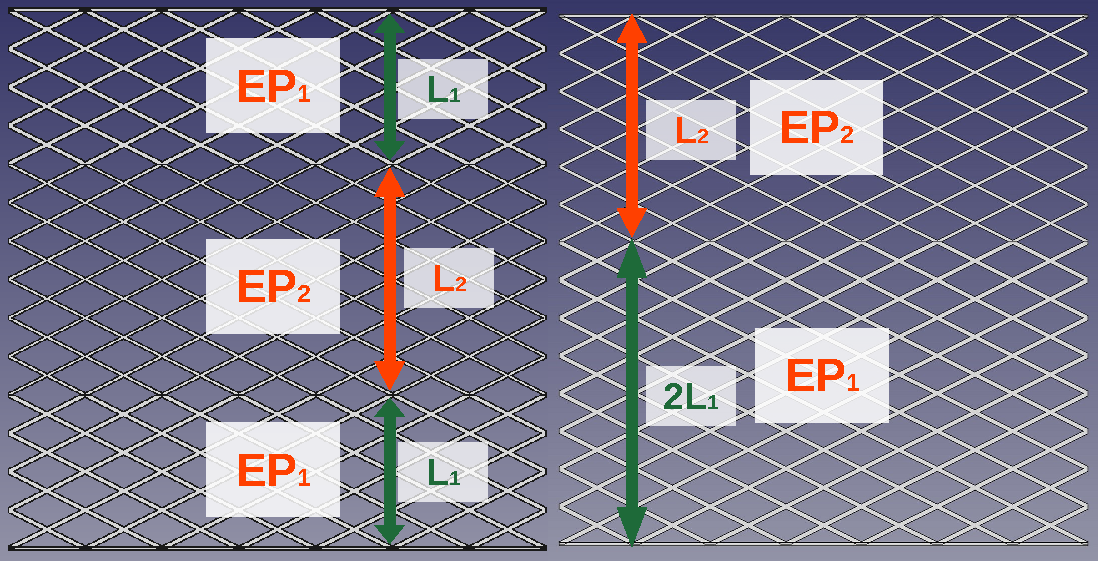
\includegraphics[width=10cm]{Images/6/symasym/symasym.pdf}\\
		\caption{Étude de l'influence de la différence entre une structure symétrique et asymétrique au travers d'une structure A à gauche (symétrique) et d'une structure B à droite (asymétrique)}
	\end{figure}
	\newpage
	
	\subsubsection{Influence de la direction de sollicitation pour une structure asymétrique}
	\hspace{0.5cm}Ayant développé des structures asymétriques, nous nous sommes interrogés sur une possible influence de la direction de sollicitation de la structure. En effet, imaginons que l'impact engendre une onde de déformation dans la structure, la réponse de celle-ci pourrait-être totalement différente suivant l'ordre des couches parcourues.\\ 
	
	Pour cela, nous avons étudié une structure asymétrique que nous avons impacté dans un sens A puis dans un sens B. Ces deux structures étant exactement identiques.
	
	%!!!!!!!!!!!!!!!!!!
	\begin{table}[H]
		\centering
		\begin{tabular}{|c|c|c|}
			\hline
			\rowcolor{Gray}
			\multicolumn{3}{c}{Structure de Référence}\\\hline
			\rowcolor{Gray}
			Couche de Gradient & Variable & Valeur\\
			\hline\hline
			& Épaisseur des Parois & 0.19 mm\\
			3 & Nombre de Losanges sur l'axe $\vec{x}$ & 7\\
			& Nombre de Losanges sur l'axe $\vec{y}$ & 1\\
			\hline
			& Épaisseur des Parois & 0.38 mm\\
			2 & Nombre de Losanges sur l'axe $\vec{x}$ & 5\\
			& Nombre de Losanges sur l'axe $\vec{y}$ & 5\\
			\hline
			& Épaisseur des Parois & 0.38 mm\\
			1 & Nombre de Losanges sur l'axe $\vec{x}$ & 4\\
			& Nombre de Losanges sur l'axe $\vec{y}$ & 6\\
			\hline
		\end{tabular}
		\caption{Paramètres de la structure Numéro ??? : Influence de la direction de sollicitation}
	\end{table}
	
	\begin{figure}[H]
		\centering
		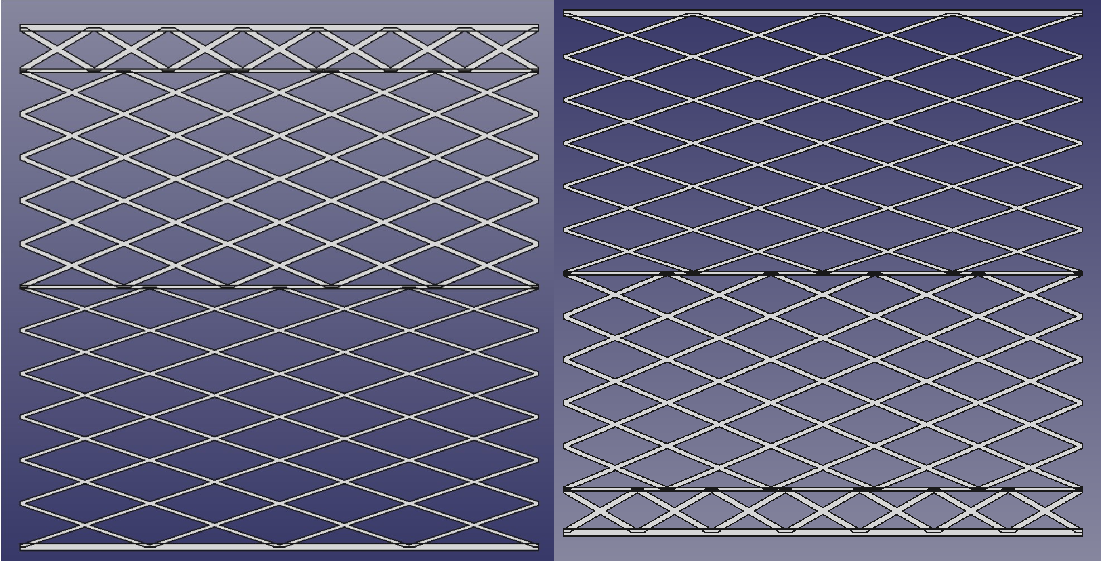
\includegraphics[width=10cm]{Images/6/directsol/directsol.pdf}\\
		\caption{Étude de l'influence de la direction de sollicitation pour une structure asymétrique}
	\end{figure}
	\newpage
	
	\section{Résultats Expérimentaux}
	\subsection{Méthode de traitement des données}
	
	\hspace{0.5cm}Pour traiter les données de nos expériences, nous avons développé notre propre logiciel de traitement de données de crash (intitulé TDC \footnote{Traitement Données Crash}). Cela a pour avantage d’avoir un logiciel parfaitement adapté à nos besoins et de totalement automatiser une tâche qui aurait dû être faite sur un tableau classique. Ainsi, sur ce logiciel, il y a la possibilité d’avoir un traitement des données avec la détection automatique du début de l’impact. Dans certains cas, cela ne fonctionne pas, on peut donc également le détecter manuellement.\\ 
	
	La démarche pour le traitement des données est la suivante : 
	Dans un premier temps nous récupérons les fichiers au format .CSV de nos expériences. Ensuite, nous chargeons ces fichiers dans TDC. Le logiciel est déjà programmé avec des paramètres de base qui fonctionnent dans le plupart des cas pour la détection du début d'impact automatique. Il permet de filtrer les données brutes de nos expériences afin de les rendre exploitables. Nous obtenons trois tracés graphiques : un graphe “Déplacement, Temps”, un graphe “Force, Temps” et un graphe “Force, Déplacements”.\\
	
	\underline{Les résultats se présentent sous la forme suivante :}\\
	
	\begin{figure}[H]
		\centering
		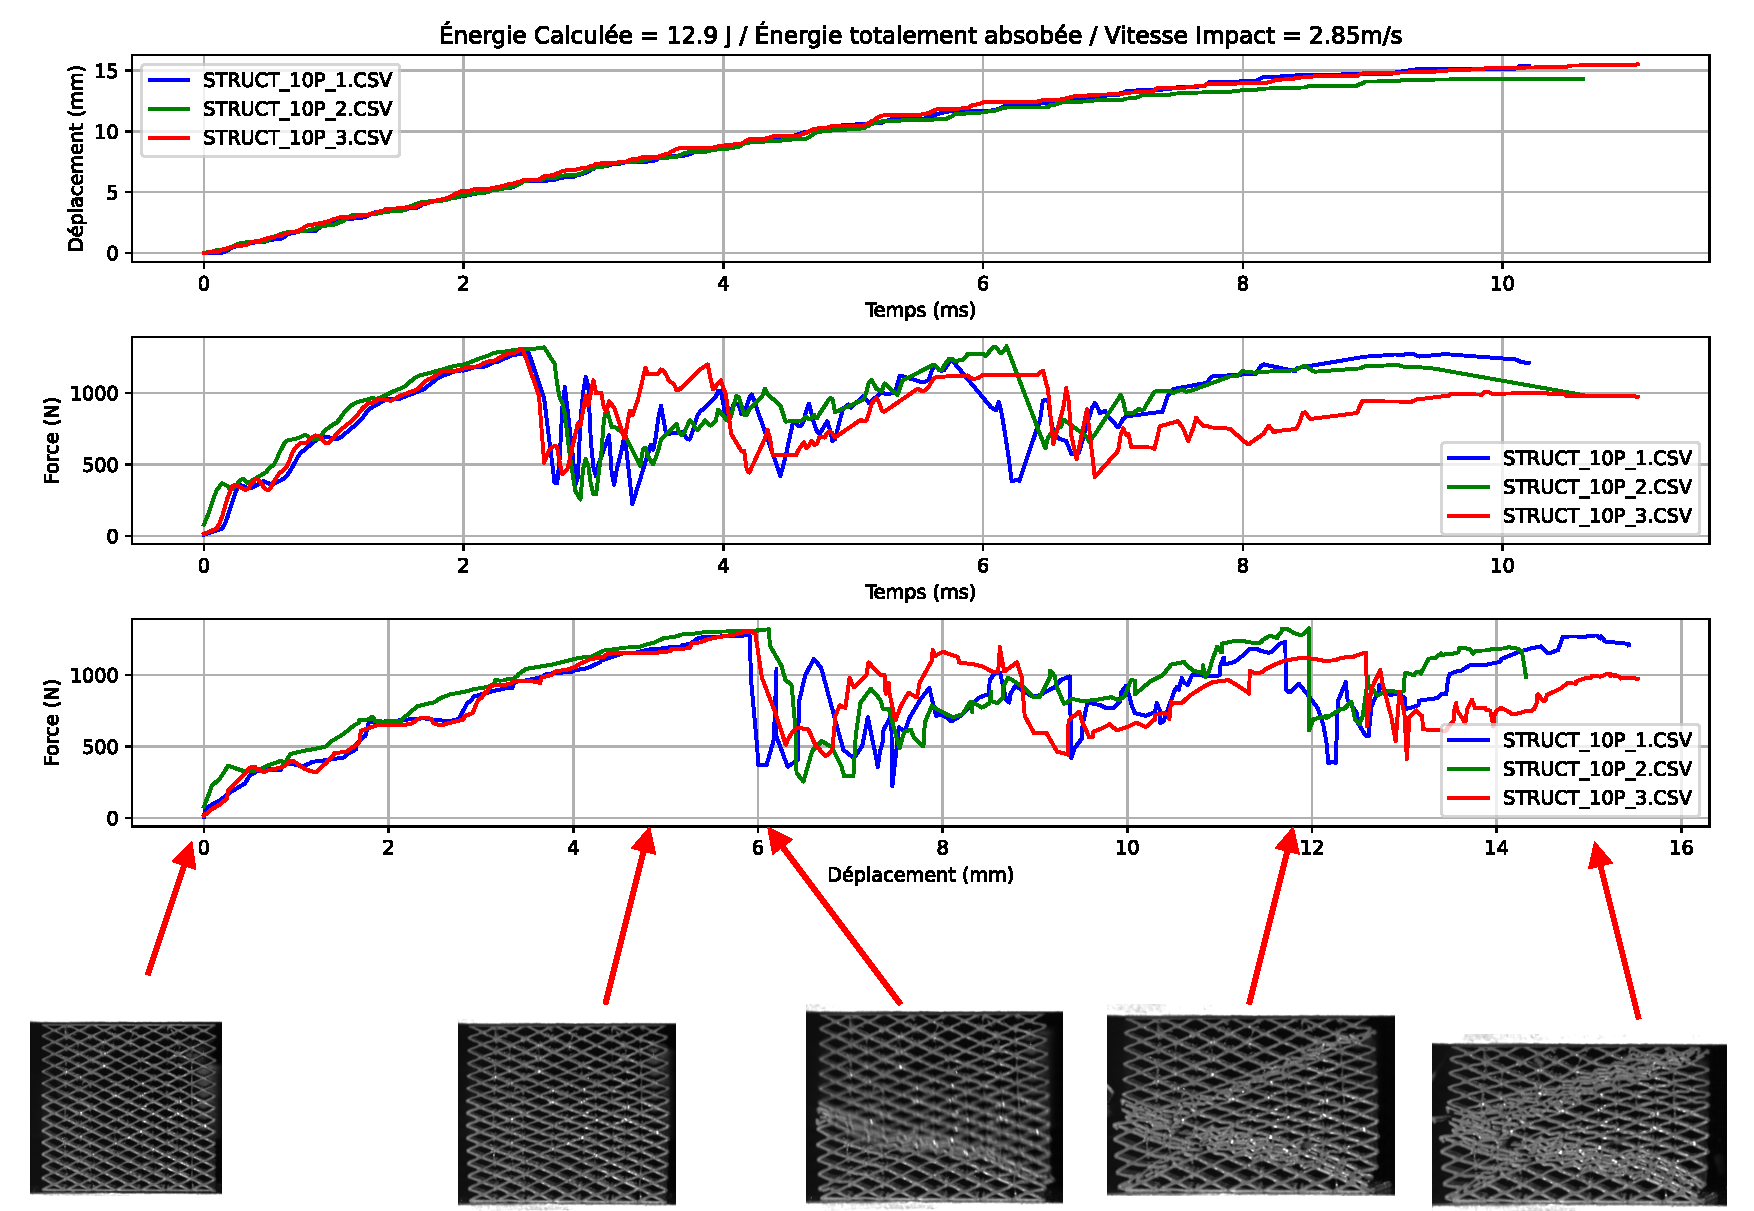
\includegraphics[width=16cm]{Images/7/7_1/TDC_STRUCT_10.pdf}
		\caption{Résultats du traitement des données pour la Structure 10}
	\end{figure}
	
	\underline{Note sur la vitesse d'impact :}\\
	
	Sur les graphes, vous pourrez remarquer que la vitesse d'impact n'est pas forcément la vitesse d'impact réelle et surtout évolue entre les graphes. Ceci est dû à l'option "suppr\_rollback" du logiciel de traitement des données. Cette option interdit le déplacement de revenir en arrière par rapport au dernier déplacement lu dans le fichier CSV. Le logiciel supprime alors beaucoup de points de données. Le calcul de la vitesse s'effectuant via la variation du déplacement par rapport au temps ($v_{moy} = \frac{\Delta d}{\Delta t}$), ce calcul est alors faussé.
	\newpage
	
	\subsection{Résultats de la géométrie N°4 : Hexagones + Triangles}
	\begin{figure}[H]
		\centering
		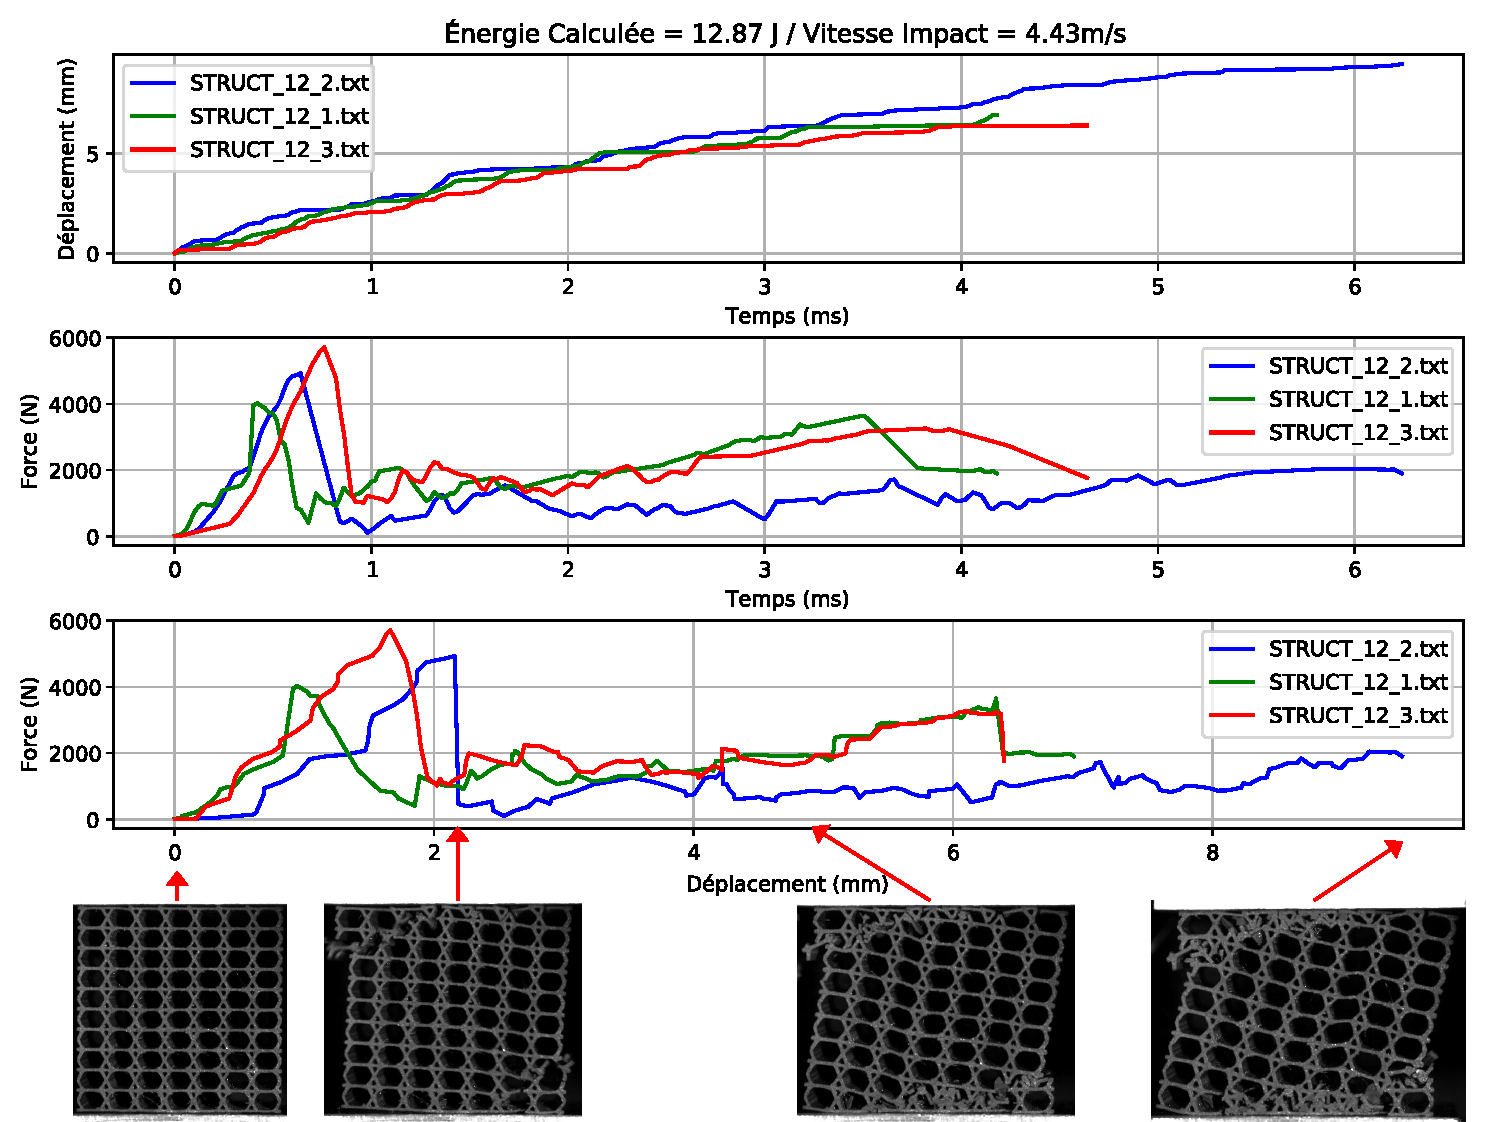
\includegraphics[width=16cm]{Images/7/7_2/STRUCT_12_AVECRUPTURE.pdf}
		\caption{Résultats du traitement des données pour la Structure 12}
	\end{figure}
	
	\hspace{0.5cm}Au vue de ces résultats, nous concluons que la géométrie est trop rigide pour absorber l'énergie d'impact de manière efficace. On remarque sur les images que la structure rompt dès lors qu'elle est en contact avec l'impacteur. Cela explique les différences entre les courbes.
	\newpage
	
	\subsection{Résultats de la géométrie N°5 : Cosinus}
	\begin{figure}[H]
		\centering
		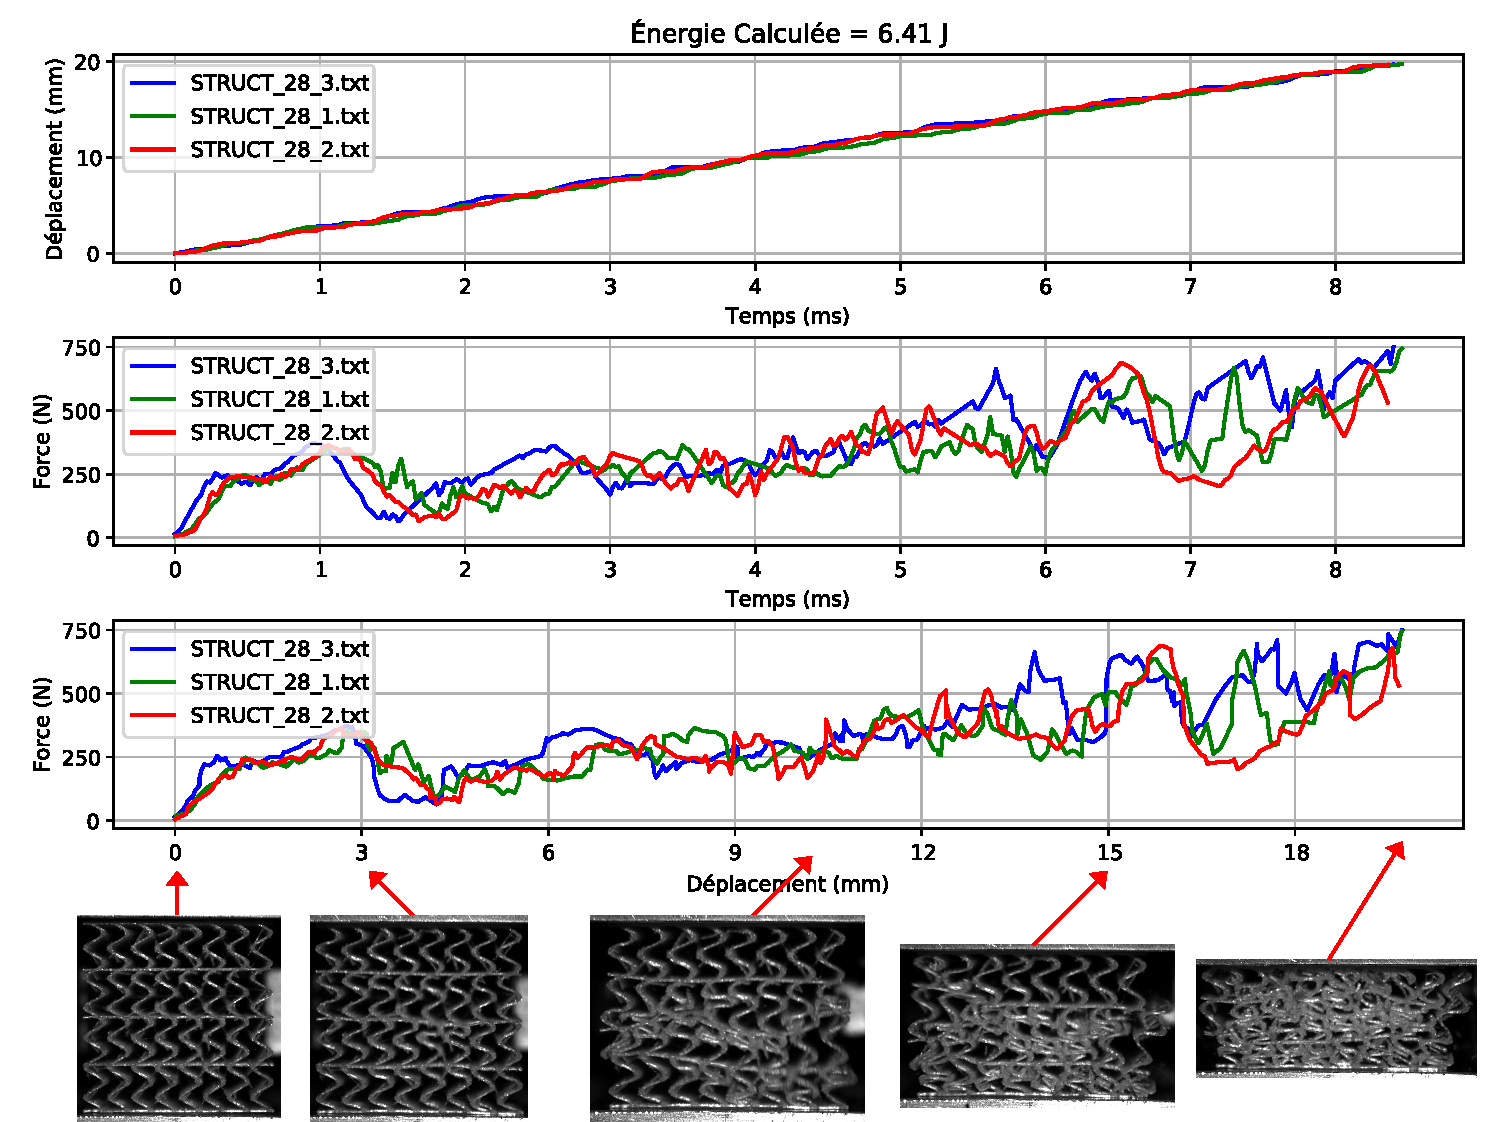
\includegraphics[width=16cm]{Images/7/7_3/STRUCT_28_AVECRUPTURE.pdf}
		\caption{Résultats du traitement des données pour la Structure 28}
	\end{figure}
	
	\hspace{0.5cm}Cette structure semble prometteuse. En effet, nous pouvons remarquer que les plateaux jouent bien leur rôle de liant évitant ainsi les cosinus de se déformer sur les côtés. Aussi, nous remarquons que les cosinus se plient en accordéon majoritairement, ce qui est nécessaire pour absorber le plus d'énergie possible.\\
	
	Par manque de temps, nous n'avons pas plus investigué des possibilités avec cette structure. Cependant, il serait intéressant de faire une étude en faisant varier les nombreux paramètres de cette structure (Voir la documentation de Lattybrides \ref{doc_lattybrides}).
	\newpage
	
	\subsection{Résultats de la géométrie N°1 : Losanges}
	\subsubsection{Influence du gradient d'épaisseur}
	
	\subsubsection{Influence du gradient de géométrie}
	
	\subsubsection{Influence de l'ajout de plateaux}
	
	\subsubsection{Influence de la direction de sollicitation sur une structure asymétrique}
	
	\subsubsection{Influence de l'épaisseur dans un gradient symétrique}
	
	\subsubsection{Comparaison de gradient symétrique et asymétrique équivalents}
	
	\subsubsection{Ajout progressif de gradient d'épaisseur}
	
	\subsubsection{Ajout progressif de losanges suivant les axes $\vec{x}$ et $\vec{y}$}
	
	\subsubsection{Comparaison de structures à gradients multiples}
	
	\hspace{0.5cm}Afin d'avoir une structure optimum qui absorbe l’énergie totale nous allons comparer plusieurs variables qui peuvent influencer le comportement des structures lattice de géométrie losange face à l’impacteur.\\
	
	\underline{Influence de la présence d'un gradient d'épaisseur}\\
	
	\begin{table}[H]
		\centering
		\begin{tabular}{|c|c|c|c|c|}
			\hline
			\rowcolor{Gray}
			Numéro de structure & 29 & 15 & 16 & 17\\
			\hline\hline
			Visuel &
			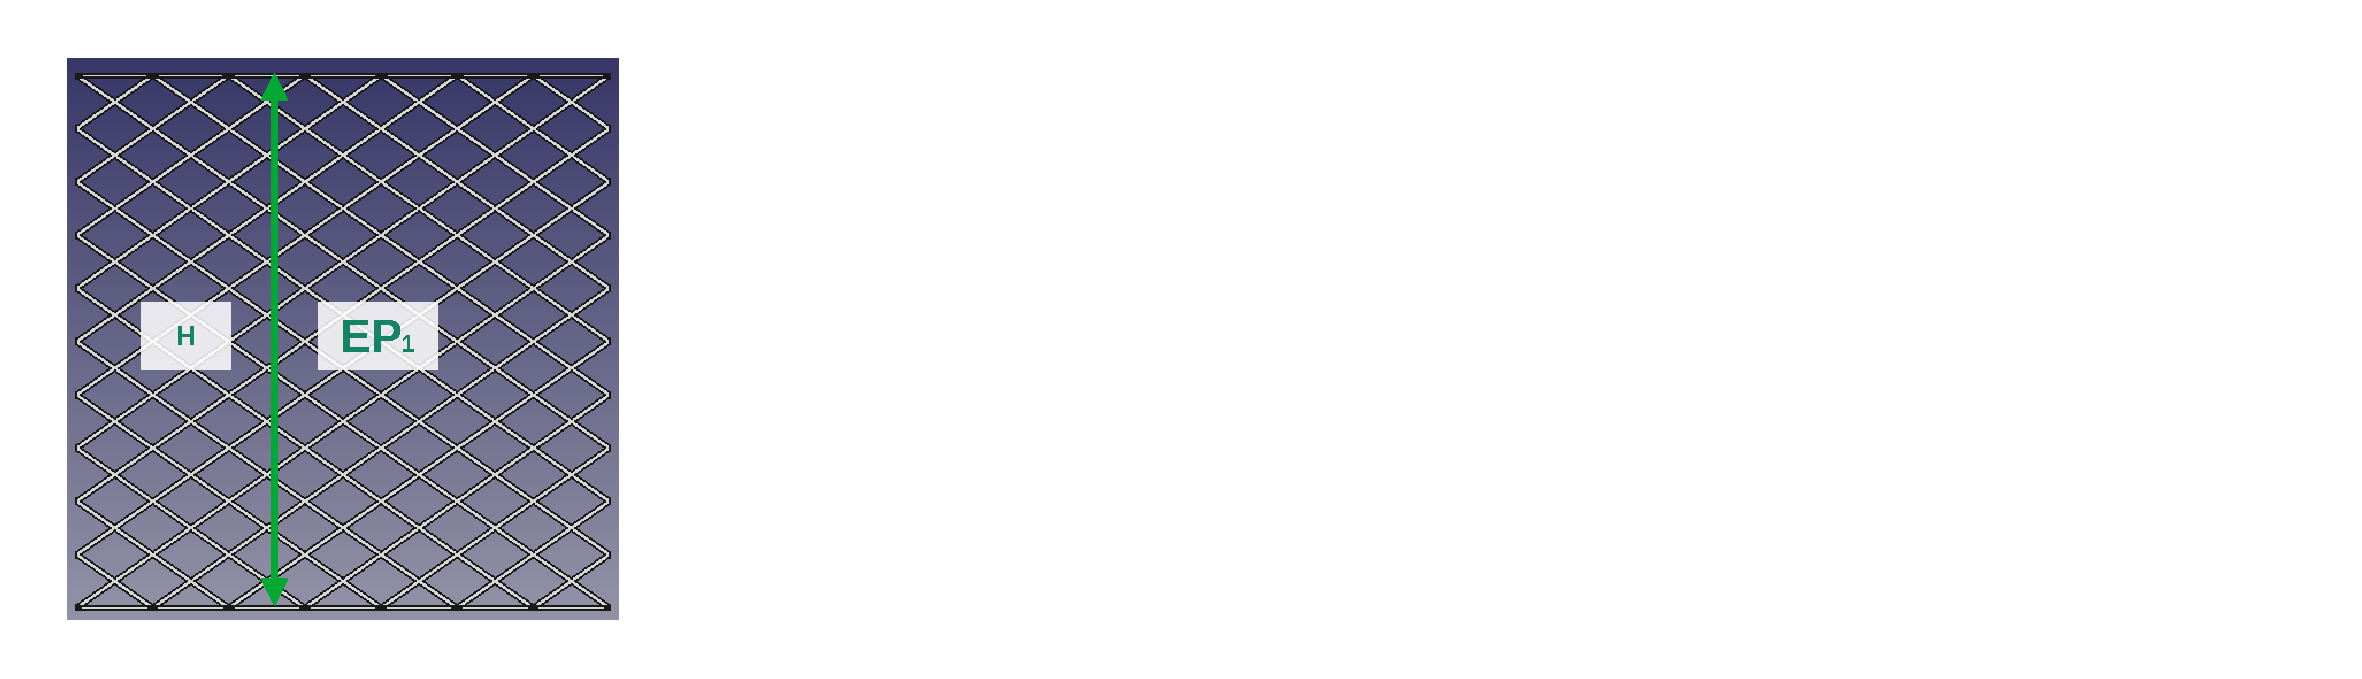
\includegraphics[width=2cm]{Images/7/1.pdf} &
			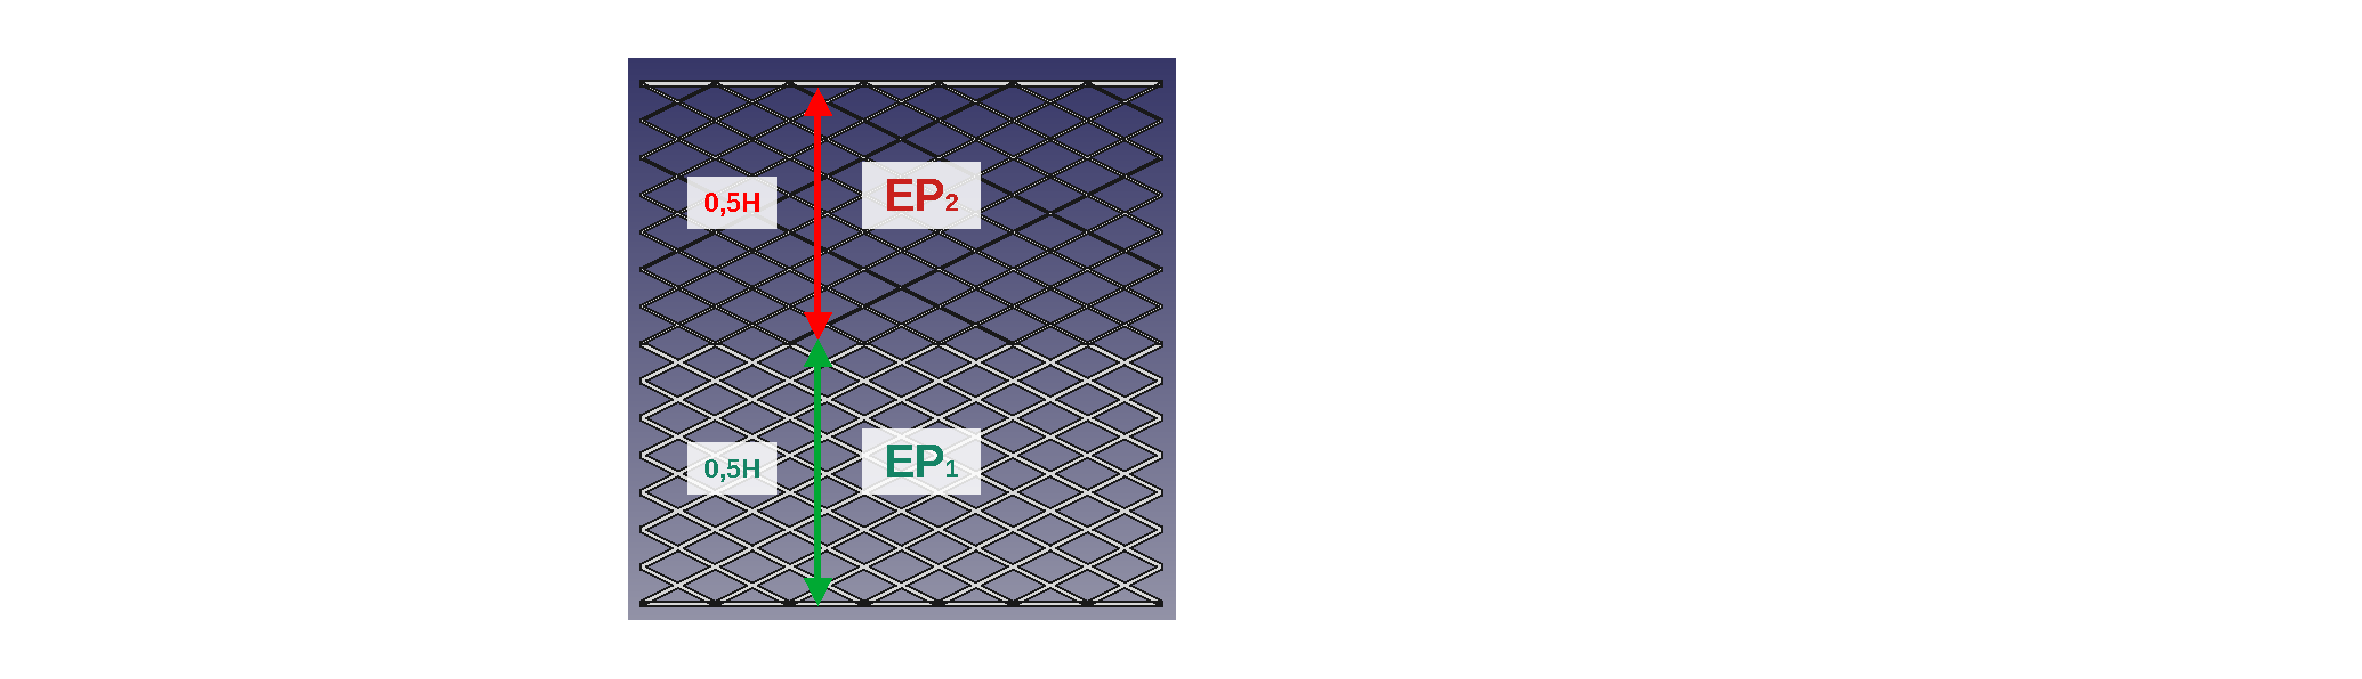
\includegraphics[width=2cm]{Images/7/15.pdf} &
			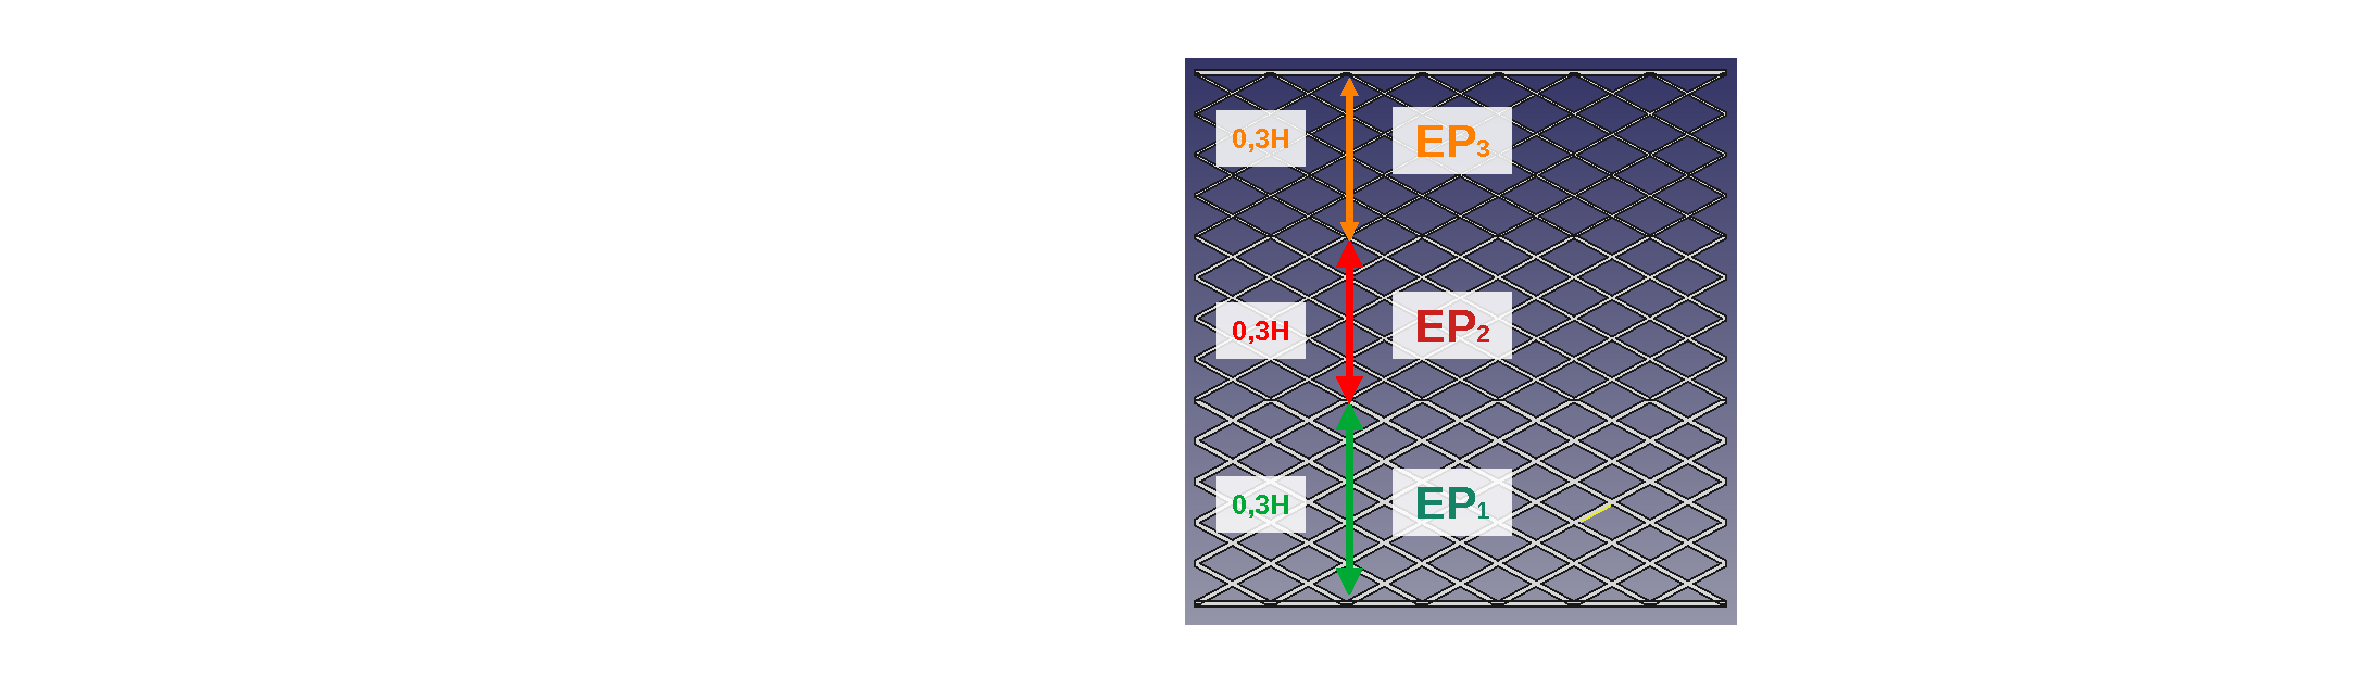
\includegraphics[width=2cm]{Images/7/16.pdf} &
			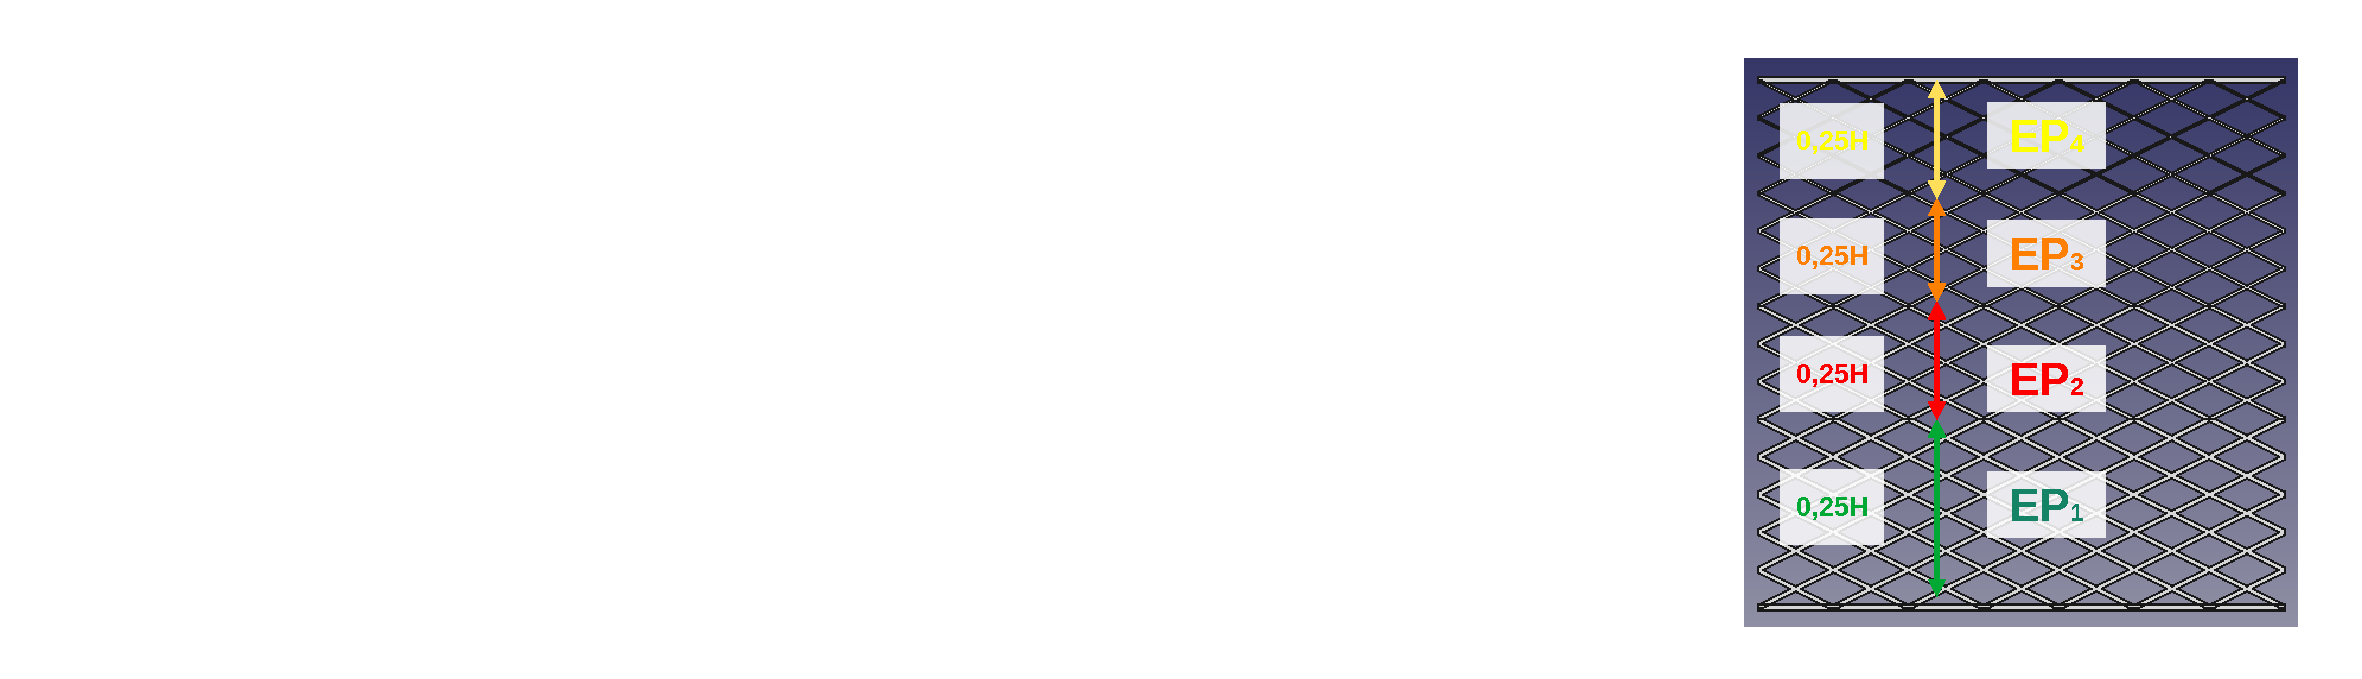
\includegraphics[width=2cm]{Images/7/17.pdf}\\
			\hline
			Energie absorbée & - & - & - & - \\
			\hline
		\end{tabular}
		\caption{Comparaison d'énergie moyenne d'absorption entre différentes épaisseurs}
	\end{table}
	
	\underline{Influence de la variation d'angle entre deux côtés}\\
	
	\begin{figure}[H]
		\centering
		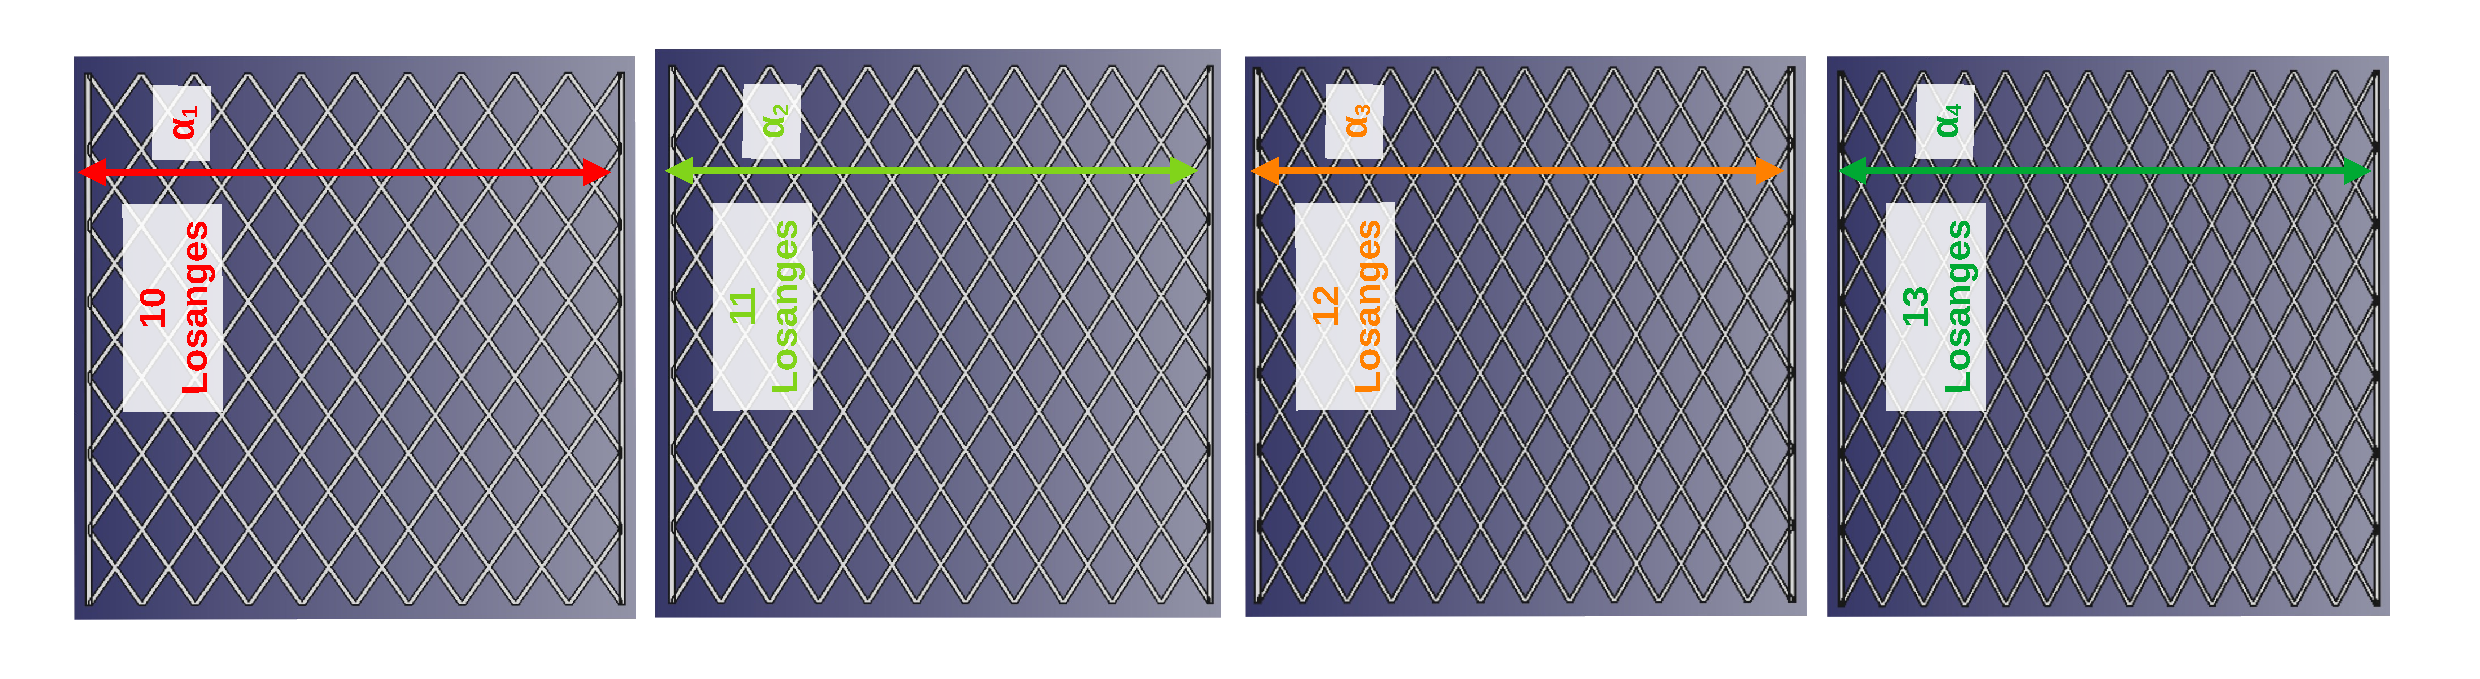
\includegraphics[width=14cm, angle=-90]{Images/7/gradient_y.pdf}
		\caption{Influence d'un gradient d'angle sur l'axe $\vec{y}$}
	\end{figure}
	
	\underline{Influence de l'ajout de plateaux}\\
	
	\begin{figure}[H]
		\centering
		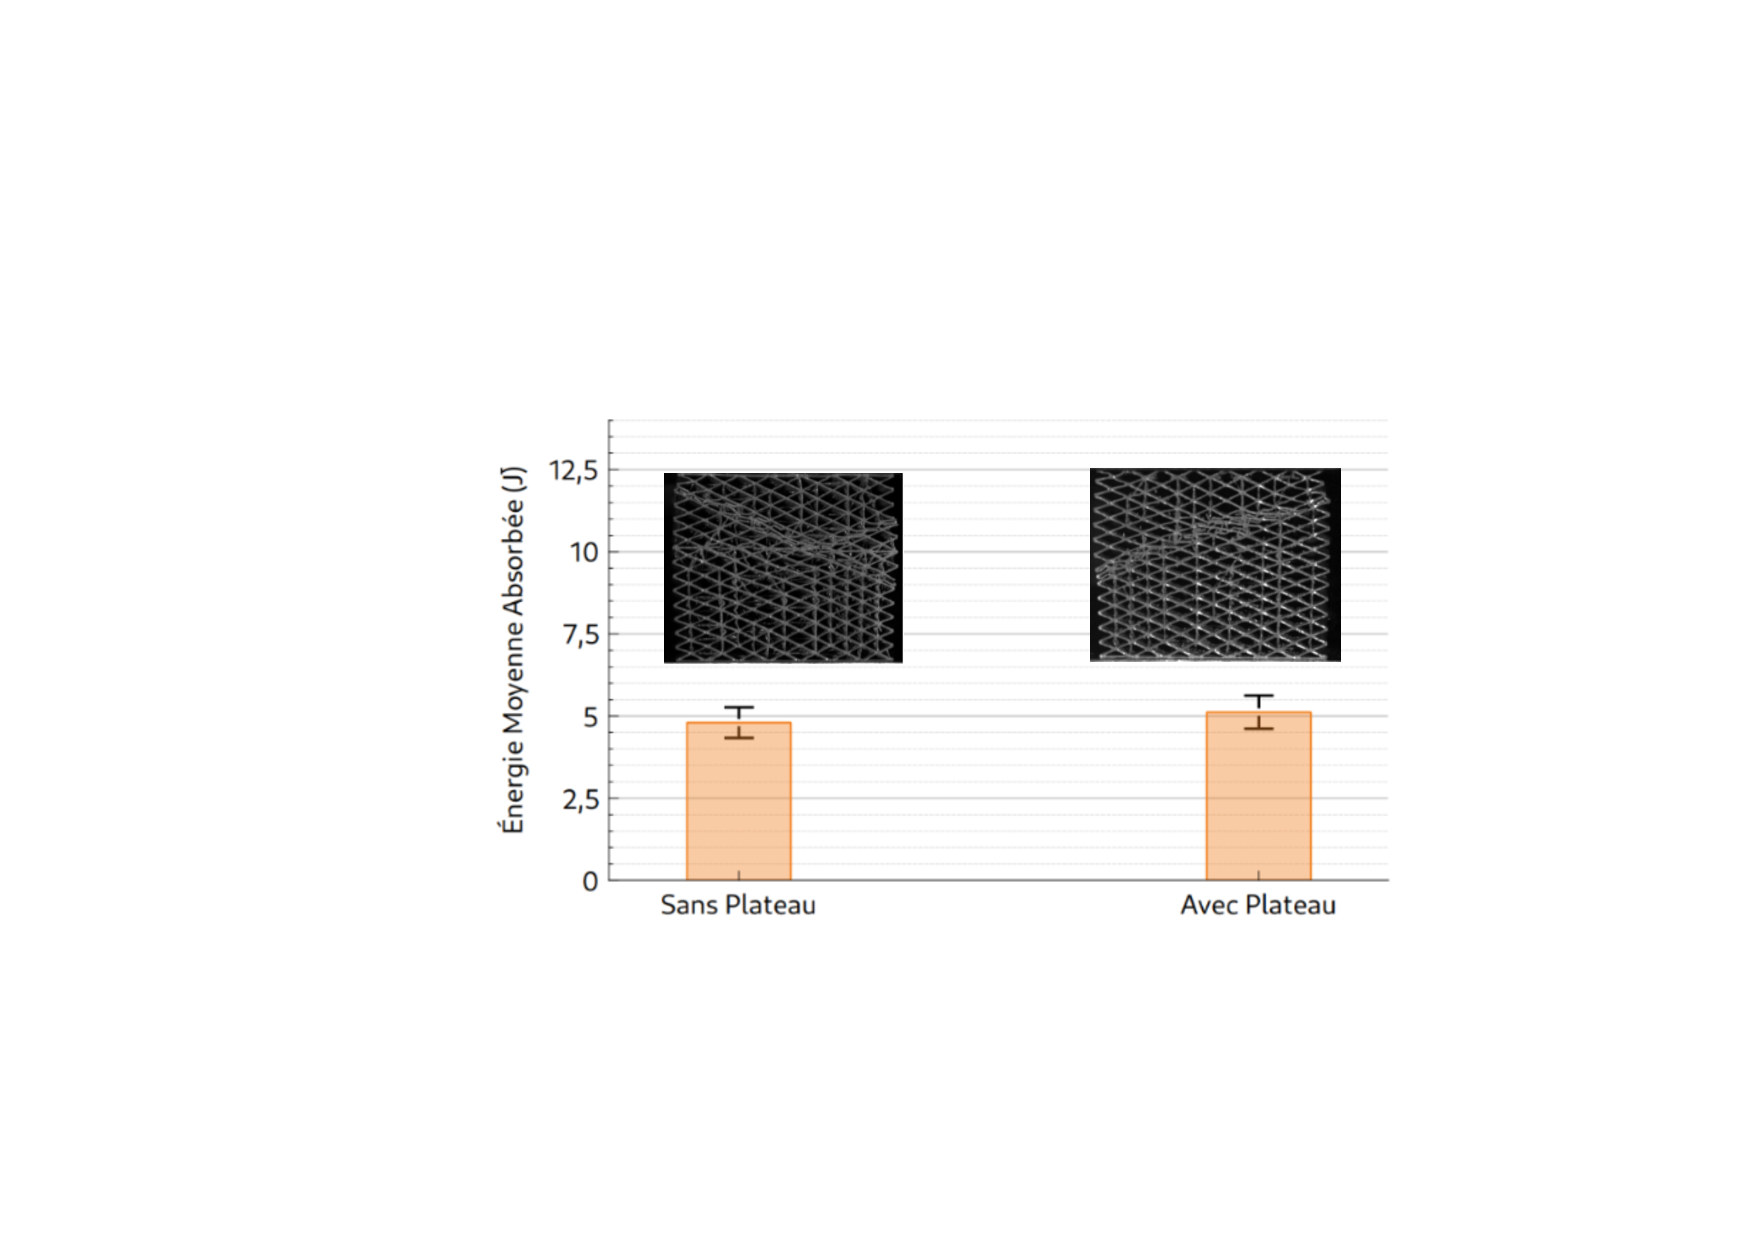
\includegraphics[width=14cm]{Images/7/plateaux.pdf}
		\caption{Influence de l'ajout de plateaux ou non}
	\end{figure}
	
	\underline{Influence d'une symétrie ou asymétrie}\\
	
	\begin{figure}[H]
		\centering
		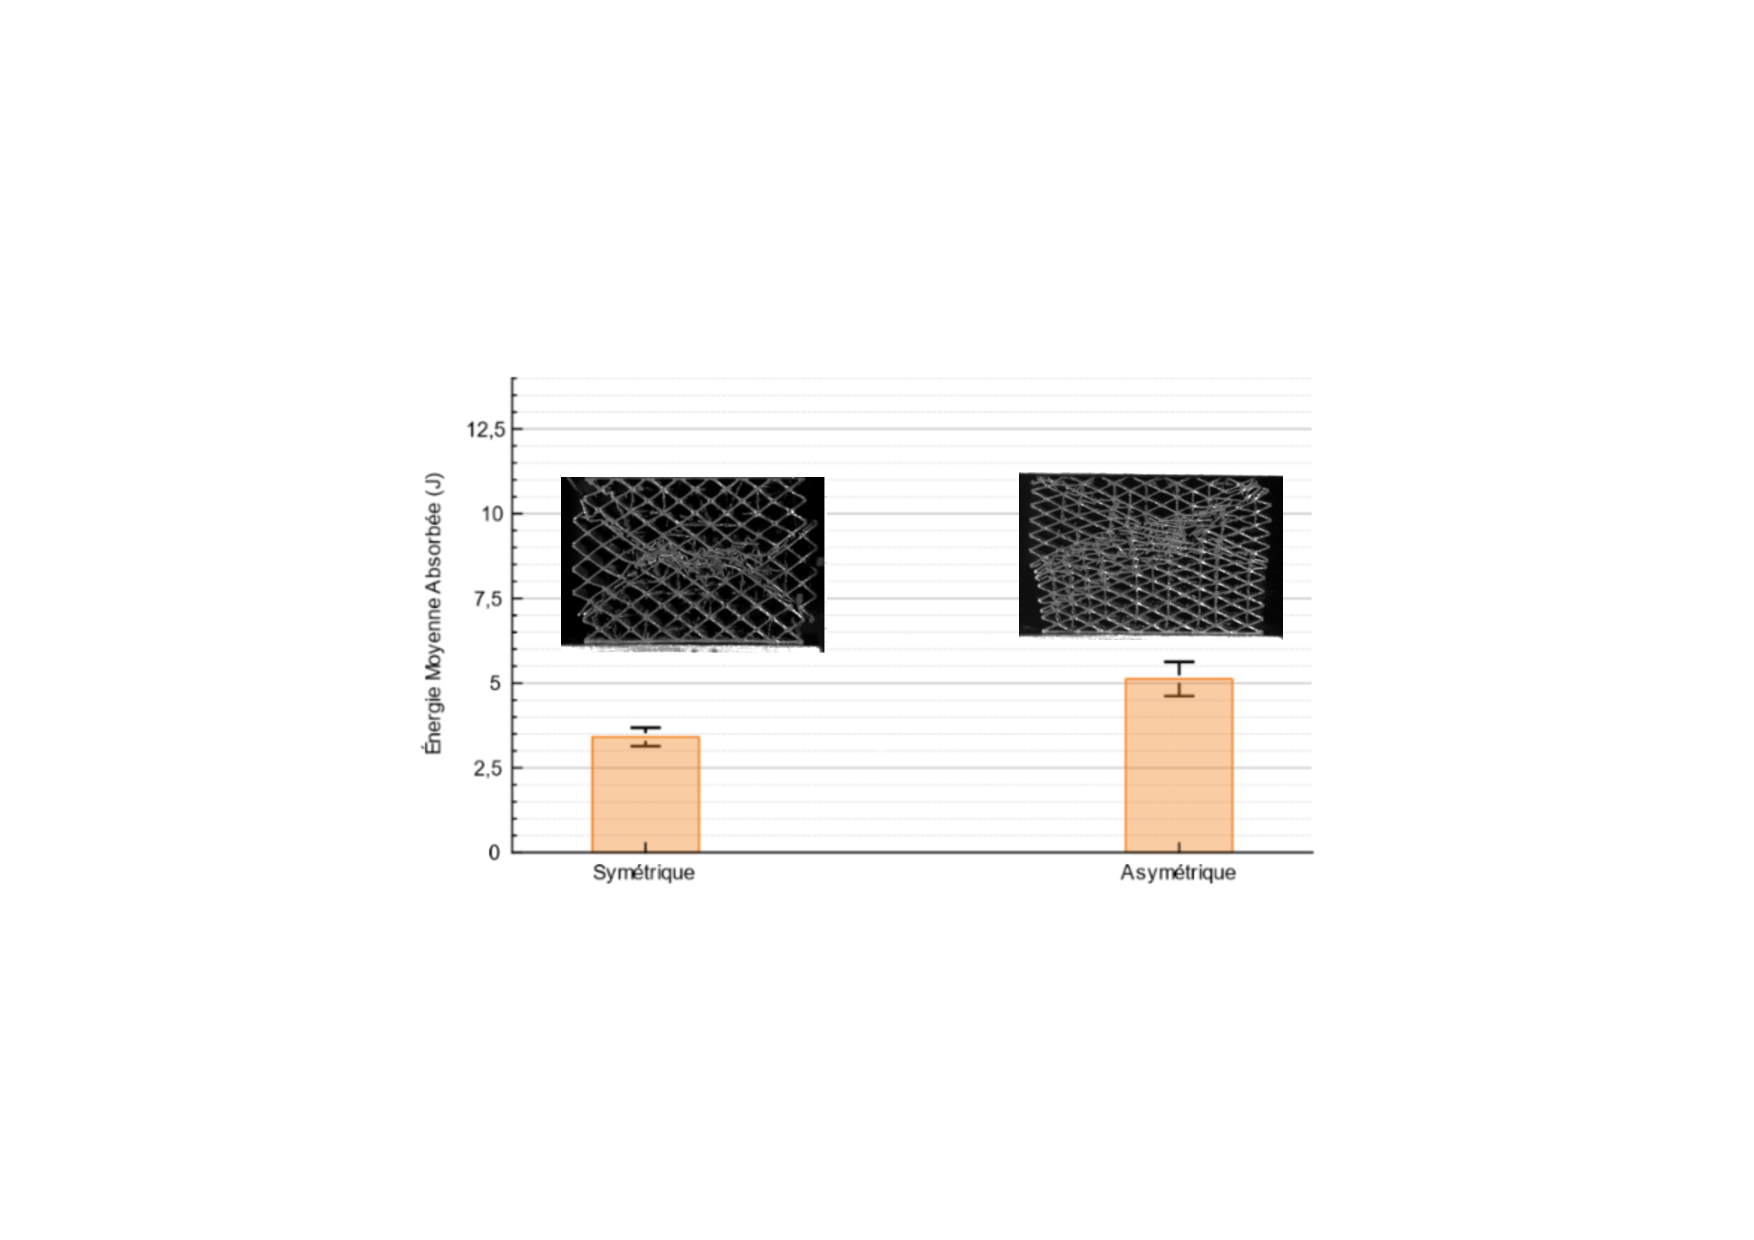
\includegraphics[width=16cm]{Images/7/sym_asym.pdf}
		\caption{Comparaison d’énergie moyenne d’absorption de la structure 3 et 9.}
	\end{figure}
	
	\underline{Influence de la direction de sollicitation}\\
	
	Dans cette partie nous allons étudier l’influence du gradient de symétrie sur l' absorption d'énergie ,en effet nous générons aussi une structure avec une géométrie asymétrique afin de comparer.
	\begin{itemize}
		\item Une structure 3 symétrique.
		\item Une structure 9 asymétrique. 
	\end{itemize}
	
	\underline{Plan d'expérience}\\
	
	Après avoir défini un par un les différents paramètres d'entrées pouvant intervenir dans l'absorption d'énergie, nous avons défini une stratégie d'expérience. Notre but était, en partant des résultats précédents, d'obtenir une structure présentant la meilleure absorption d'énergie.
	\newpage
	
	\section{Modèle numérique}
	\subsection{Maillage}
	\subsubsection{Structure}
	
	\hspace{0.5cm}Il n’est malheureusement pas possible de mailler les structures générées de manière automatique avec un maillage de tétraèdres par exemple. En effet, pour faciliter la génération des structures sur \textit{FreeCAD}, le modèle 3D des structures est séparé entre de multiples entités. Le “Body” est le corps de la pièce, c’est l’objet contenant toutes les autres entités de la pièce. Les “Pad” sont toutes les extrusions des modèles 2D “Sketch”. Pour faciliter le développement de l’atelier de génération des structures, il a été choisi de faire une seule esquisse (“Sketch”) par plateaux et par couches de gradients. Cependant, lors de l’exportation du modèle 3D au format STEP, la structure apparaît en plusieurs parties non liées entre elles.
	
	\begin{figure}[H]
		\centering
		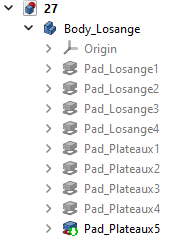
\includegraphics[height=6cm]{Images/8/8_1/arborescence_freecad.png}
		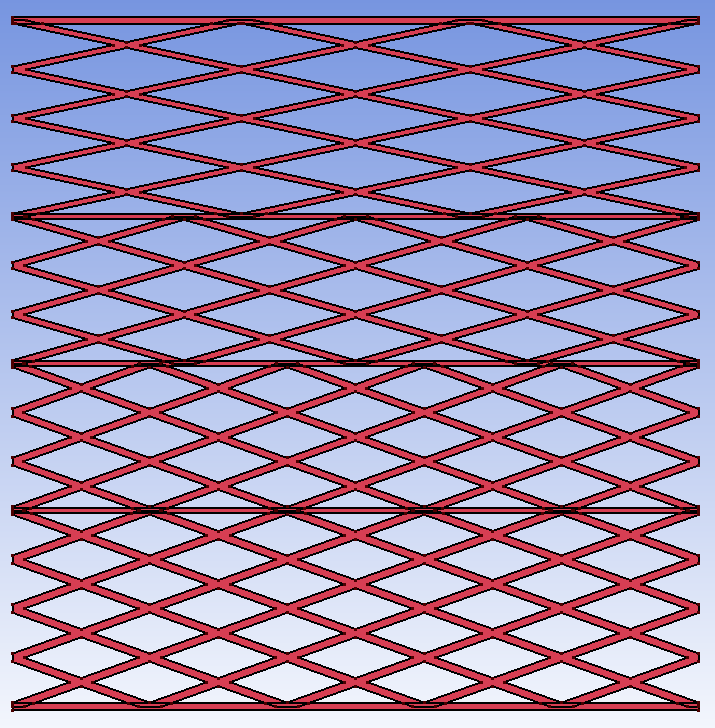
\includegraphics[height=6cm]{Images/8/8_1/step_lsdyna.png}\\
		\caption{Arborescence du fichier \textit{FreeCAD} pour la structure 27 et importation du fichier STEP sur \textit{LsDyna} (Présence de jointures entre les couches de gradients et les plateaux)}
	\end{figure}
	
	\hspace{0.5cm}Afin de mailler une structure unique, nous avons utilisé \textit{HyperWorks}. La première étape a été d’importer le fichier STEP sur le logiciel. Par défaut, \textit{HyperWorks} décompose le fichier STEP en une multitude de facettes. Le but est de supprimer toutes les facettes qui ne sont pas sur le plan xOy dans le but de réaliser un maillage unifié.
	
	\begin{figure}[H]
		\centering
		\includegraphics[height=6cm]{Images/8/8_1/hm_step.png}
		\includegraphics[height=6cm]{Images/8/8_1/hm_xoy.png}\\
		\caption{Importation du fichier STEP sur \textit{\textit{HyperWorks}} et suppression des facettes qui ne sont pas sur le plan xOy}
	\end{figure}
	\newpage
	
	\hspace{0.5cm}Une fois extraites, nous avons sélectionné les surfaces de la structure sur le plan xOy et nous avons créé une esquisse recevant la structure comme projection. Sur cette esquisse, on remarque des traits horizontaux indésirables. Nous devons alors les supprimer afin de fusionner les différentes parties de la structure. Une fois fait, les traits dessinés sont des traits de construction qui doivent-être passés en traits pleins pour pouvoir générer une surface.
	
	\begin{figure}[H]
		\centering
		\begin{tabular}{m{10cm}m{6cm}}
			\includegraphics[height=3cm]{Images/8/8_1/hm_lignes_construction.png} & \includegraphics[height=6cm]{Images/8/8_1/hm_traits_pleins.png}\\
		\end{tabular}
		\caption{Projection de la structure sur une esquisse et création d’une surface fusionnée, suppression des lignes de construction (lignes sélectionnées) et conversion des lignes de construction en traits pleins.}
	\end{figure}
	
	\hspace{0.5cm}Maintenant que nous avons une unique surface, il est assez aisé de la mailler. Pour ce faire, dans le menu \textit{HyperMesh}, nous sélectionnons la fonctionnalité “automesh” dans l'onglet “2D” en sélectionnant des éléments quadrilatères uniquement de taille 0.15 mm. Il ne reste plus qu’à exporter le maillage 2D sur \textit{LsDyna} au format *.k.
	
	\hspace{0.5cm}Sur \textit{LsDyna}, l'élément shell est modélisé par une épaisseur suivant $\vec{z}$ de $1 mm$ en déformations planes (ELFORM = 13). L'hypothèse de déformations planes permet de sauver un temps de calcul plutôt élevé ($3 h$ de calcul avec un solide de $1 mm$ d'épaisseur suivant $\vec{z}$ contre $14 min$ avec l'hypothèse de déformations planes). Afin d'obtenir une bonne précision de calcul, nous avons paramétré l'élément shell pour qu'il ait $5$ points d'intégration dans l'épaisseur (NIP = 5). Nous avons également utilisé l'option *CONTROL\_SHELL afin de paramétrer l'ajout de points d'intégrattion de Lobatto sur les peaux des éléments shells (INTGRD = 1).
	
	\subsubsection{Impacteur}
	
	\hspace{0.5cm}L’impacteur est quant à lui modélisé par un shell d’épaisseur $1 mm$ positionné à $2 mm$ (fibre neutre) du haut de la structure et débordant de $5 mm$ de part et d'autre de la structure. Un maillage quadrilatère de dimension x = 100 subdivisions et y = 1 subdivision est choisi. L'épaisseur de l'élément shell choisie est de $1 mm$ suivant $\vec{z}$ avec des éléments en déformations planes (ELFORM = 13).
	
	\begin{figure}[H]
		\centering
		\includegraphics[width=16.5cm]{Images/8/8_1/ls_impacteur.png}
		\caption{Impacteur modélisé par une shell de $1 mm$ d’épaisseur suivant $\vec{z}$ et maillée par des éléments quadrilatères (100x1 subdivisions) avec l'hypothèse de déformations planes}
	\end{figure}
	\newpage
	
	\subsection{Paramétrage du calcul}
	\subsubsection{Système d'Unités}
	\hspace{0.5cm}Avec le fichier de maillage de la structure, nous sommes contraints de travailler avec le millimètre comme unité de longueur. Au vu de la rapidité de l’impact, il est judicieux de choisir la milliseconde comme unité de temps.
	
	\hspace{0.5cm}\underline{En appliquant la $2^{e}$ loi de Newton on trouve l’unité de masse complémentaire du système d’unité :}
	
	$$\sum{F} = m\gamma \Rightarrow N = \frac{kg * m}{s^{2}} = kg * \frac{m}{s^{2}} \Rightarrow ?kg * \frac{10^{3}mm}{10^{6}ms^{2}} = \frac{?kg * 10^{3}mm}{10^{6}ms^{2}}$$
	
	\hspace{0.5cm}\underline{Afin d'obtenir des Newton en unité de force, nous passons l'unité de masse au gramme :}
	
	$$10^{3}g * \frac{10^{3}mm}{10^{6}ms^{2}} = \frac{10^{3}g * 10^{3}mm}{10^{6}ms^{2}}$$
	
	\hspace{0.5cm}\underline{Les unités utilisées sont donc les suivantes :}
	
	\begin{table}[!h]
		\centering
		\begin{tabular}{|c|c|}
			\hline
			\rowcolor{Gray}
			\textbf{Type de Grandeur} & \textbf{Unité choisie}\\\hline\hline
			Masse & Gramme ($g$)\\\hline
			Longueur & Millimètre ($mm$)\\\hline
			Temps & Milliseconde ($ms$)\\\hline
			Force & Newton ($N$)\\\hline
			Contrainte & Mégapascal ($MPa$)\\\hline
		\end{tabular}
		\caption{Système d'unités utilisé dans \textit{LsDyna}}
	\end{table}
	
	\subsubsection{Matériau et Pièces}
	\hspace{0.5cm}\underline{Propriétés matérielles de la structure :}\\
	
	\hspace{0.5cm}Nous avons tout d'abord tenté d'utiliser une loi de comportement du type Johnson-Cook pour modéliser les propriétés matérielles du PLA\footnote{Acide Polylactique}. En effet, lors de cette expérience, la structure va subir une très grande déformation élastique mais aussi plastique. C'est pour cela que nous avons besoin d'un modèle incluant la plastification pour modéliser correctement les propriétés matérielles du PLA.
	
	\begin{table}[!h]
		\centering
		\begin{tabular}{|c|c|}
			\hline
			\rowcolor{Gray}
			\textbf{Grandeur} & \textbf{Valeur}\\\hline\hline
			& \\
			Masse Volumique & $\rho = 1.24g/cm^{3} = 1.24 \frac{g}{10^{3}mm^{3}} = 1.24e^{-3} g/mm^{3}$\\
			& \\\hline
			& \\
			Module de Young & $E = 1 390 MPa = 1 390 \frac{N}{mm^{2}}$\\
			& \\\hline
			& \\
			Coefficient de Poisson & $\nu = 0.35$\\
			& \\\hline
			& \\
			Coefficients de la loi de Johnson-Cook & $A = 68.55 MPa$, $B=960.43 MPa$, $n=5.37$, $C=0.25$\\
			& \\\hline
		\end{tabular}
		\caption{Propriétés matérielles de la structure en PLA}
	\end{table}
	
	\hspace{0.5cm}La loi de comportement Johnson-Cook exprimées ci-dessus ont étés trouvés sur internet dans les deux articles suivants : \cite{JC_PLA1},  \cite{JC_PLA2}. Après plusieurs essais de calculs, nous avons abandonné cette loi, donnant des valeurs d'efforts 7 à 8 fois supérieurs aux valeurs expérimentales. Nous avons alors utilisé un modèle de matériau purement élastique (*MAT\_ELASTIC) avec un Module de Young $E = 4 000 MPa$. La valeur du Module de Young peut paraître élevée pour du PLA mais elle a été ajustée dans le but de diminuer les efforts maximum subits par la structure.\\
	
	\hspace{0.5cm}Ces propriétés matérielles ne sont évidement pas représentatives du matériau réellement utilisé. L'établissement d'une loi de comportement avec le PLA provenant de notre fournisseur \textit{Grossiste3D} aurait été nécessaire.
	\newpage
	
	\hspace{0.5cm}\underline{Propriétés matérielles de l'impacteur :}
	
	\begin{table}[!h]
		\centering
		\begin{tabular}{|c|c|}
			\hline
			\rowcolor{Gray}
			\textbf{Grandeur} & \textbf{Valeur}\\\hline\hline
			& \\
			Masse Volumique & $\rho = 7810kg/m^{3} = 7810 \frac{10^{3}g}{10^{9}mm^{3}} = 7.81e^{-3} g/mm^{3}$\\
			& \\\hline
			& \\
			Module de Young & $E = 210 000 MPa = 210 000 \frac{N}{mm^{2}}$\\
			& \\\hline
			& \\
			Coefficient de Poisson & $\nu = 0.3$\\
			& \\\hline
			& \\
			Masse & $m = 3344.65 g$\\
			& \\\hline
		\end{tabular}
		\caption{Propriétés matérielles de l'impacteur}
	\end{table}
	
	\hspace{0.5cm}Les propriétés matérielles de l'impacteur ne sont pas très importantes. En effet, l'inertie de l'impacteur ne va être uniquement conditionnée par le paramètre *ELEMENT\_MASS\_PART de \textit{LsDyna}. Cette option nous permet de renseigner la masse de l'impacteur en s'affranchissant de la valeur de la masse volumique précédemment renseignée (la masse volumique doit nécessairement être renseignée pour ne pas générer d'erreurs par le solveur). L'impacteur est modélisé avec un matériau rigide (*MAT\_RIGID).
	
	\subsubsection{Contacts}
	\hspace{0.5cm}Deux contacts sont nécessaires dans ce problèmes, le contact entre l'impacteur et la structure ainsi que le contact entre la structure et elle-même (lorsque la structure est totalement écrasée). Le contact entre l'impacteur et la structure est défini entre deux pièces (SURFTYP\_A = SURFTYP\_B = 3) par l'option\newline *CONTACT\_2D\_AUTOMATIC\_SURFACE\_TO\_SURFACE sans coefficient de friction. Pour le contact entre la structure et elle-même, il est nécessaire de créer un *SET\_PART au préalable. Le contact utilisé est alors définit entre les deux sets (SURFTYP\_A = SURFTYP\_B = 2) par l'option\newline  *CONTACT\_2D\_AUTOMATIC\_SINGLE\_SURFACE sans coefficient de friction.
	
	\subsubsection{Conditions Initiales et Conditions aux Limites}
	\hspace{0.5cm}\underline{Vitesse d'impact :}\\
	
	\hspace{0.5cm}L'énergie d'impact calculée précédemment (\ref{energie_impact}) est de $E_{p} = 13.7 J$. Avant de toucher la structure, toute l'énergie potentielle de l'impacteur se transforme en énergie cinétique.\\
	
	\underline{On obtient alors la vitesse de l'impacteur via la relation :}
	$$E_{c} = \frac{1}{2}mv^{2} \Rightarrow v = \sqrt{\frac{2E_{c}}{m}} = \sqrt{\frac{2 * 13.7}{3344.65}} = 2.86 m/s = 2.86 mm/ms$$
	
	La vitesse initiale de l'impacteur est alors renseignée dans LsDyna via l'option\newline *INITIAL\_VELOCITY\_RIGID\_BODY.\\
	
	\underline{Masse de l'Impacteur :}\\
	
	Notre problème n'est modélisé que sur $1 mm$ d'épaisseur contrairement à $40 mm$ expérimentalement. L'énergie d'impact doit donc être diminuée par 40. D'après la formule de l'énergie cinétique $E_{c} = \frac{1}{2}mv^{2}$, diviser la masse par 40 revient donc à diviser l'énergie d'impact par 40 également. La masse de l'impacteur renseignée dans \textit{LsDyna} est donc $\frac{m}{40} = \frac{3344.65}{40} = 83.62 g$.\\
	
	\underline{Condition de maintiens de la structure à sa base :}\\
	
	La façon la plus simple de récupérer les informations de force sous la structure serait d'effectuer un contact entre un élément shell sous la structure et la structure elle-même. Cependant, ceci engendre un coût de calcul supplémentaire que nous pouvons éviter avec l'option *RIGIDWALL\_PLANAR de \textit{LsDyna}. Cette option créer un mur rigide où nous pourrons récupérer les forces facilement sans gérer de contact.
	
	\subsubsection{Amélioration de la Rapidité du Calcul}
	\hspace{0.5cm}Les calculs étant relativement lourds, nous avons choisi d’utiliser une option de \textit{LsDyna} qui s’appelle le “mass scaling”. Pour que le solveur de \textit{LsDyna} converge, le pas de temps de calcul est calculé de cette façon \cite{LS_TIMESTEP} :
	
	\begin{equation}
		\Delta t = fact_{\Delta t} \frac{L}{c} \leq \Delta t ^{crit} = \frac{2}{\omega_{max}}
		\label{dt_crit}
	\end{equation}
	
	\begin{itemize}
		\item $L$ : Dimension caractéristique de l'élément le plus petit du modèle. Pour un élément shell il s'agit de la diagonale.
		\begin{center}
			\includegraphics[height=2cm]{Images/8/8_2/shell_L.pdf}
		\end{center}
		\item $c$ : Vitesse du son dans le matériau. Pour un élément shell, le son dans l'élément suit cette expression :
		$$c = \sqrt{\frac{E}{\rho (1 - \nu^{2})}}$$
		Où $E$ est le Module de Young, $\rho$ la masse volumique de l'élément et $\nu$ le coefficient de poisson du matériau.
		\item $fact_{\Delta t}$ : Facteur de sécurité utilisé pour être sûr que le pas de temps calculé $\Delta t$ soit inférieur au pas de temps critique $\Delta t ^{crit}$. Dans \textit{LsDyna} le paramètre $fact_{\Delta t}$ est représenté par la variable TSSFACT.
		\item $\Delta t ^{crit}$ : Est le pas de temps critique à ne pas dépasser pour que le solveur puisse converger.
		\item $\omega_{max}$ : Correspond à la plus grande fréquence propre du modèle élément finis.
	\end{itemize}
	
	\hspace{0.5cm}Dans cette formule \ref{dt_crit}, la masse volumique intervient directement au numérateur du pas de temps calculé donc la masse du modèle intervient également au numérateur :
	
	$$\Delta t = fact_{\Delta t} \frac{L}{c} = fact_{\Delta t} L \sqrt{\frac{\rho (1 - \nu^{2})}{E}} = fact_{\Delta t} L \sqrt{\frac{m (1 - \nu^{2})}{EV}}$$
	\hspace{0.2cm}
	
	\hspace{0.5cm}L'option de "mass scaling" de \textit{LsDyna} va artificiellement augmenter la masse du modèle dans le but d'augmenter le pas de temps de calcul. Cependant, une augmentation trop importante (supérieure à $3\%$) est dangereuse à cause des effets d'inertie qui ne seront plus du tout les mêmes qu'expérimentalement.
	
	\hspace{0.5cm}Dans notre cas, nous avons utilisé l'option de "mass scaling" à hauteur de $1.9484\%$ c'est à dire une masse ajoutée de $1.6481g$ pour une masse totale de $84.589g$. Nous avons vérifié que l'option de "mass scaling" n'engendre pas une augmentation de l'énergie cinétique de l'impacteur.
	\newpage
	
	\subsection{Écart avec les expériences}
	\begin{figure}[!h]
		\centering
		\begin{tabular}{m{3cm}m{6cm}m{6cm}}
			Instant 0 & \includegraphics[width=5cm]{Images/8/8_3/exp1.png} & \includegraphics[width=5cm]{Images/8/8_3/ef1.png}\\
			Instant 1 & \includegraphics[width=5cm]{Images/8/8_3/exp2.png} & \includegraphics[width=5cm]{Images/8/8_3/ef2.png}\\
			Instant 2 & \includegraphics[width=5cm]{Images/8/8_3/exp3.png} & \includegraphics[width=5cm]{Images/8/8_3/ef3.png}\\
			Instant 3 & \includegraphics[width=5cm]{Images/8/8_3/exp4.png} & \includegraphics[width=5cm]{Images/8/8_3/ef4.png}\\
			Instant 4 & \includegraphics[width=5cm]{Images/8/8_3/exp5.png} & \includegraphics[width=5cm]{Images/8/8_3/ef5.png}\\
			Instant 5 & \includegraphics[width=5cm]{Images/8/8_3/exp6.png} & \includegraphics[width=5cm]{Images/8/8_3/ef6.png}\\
		\end{tabular}
		\caption{Comparaison des résultats Expérimentaux - Éléments Finis à divers instants de déformation de la structure (Structure 11).}
		\label{exp_vs_ef}
	\end{figure}
	
	\begin{figure}[H]
		\centering
		\includegraphics[width=15.5cm]{Images/8/8_3/comparaison_EXP_EF_ELASTIC_E4000_DEP19_73.pdf}
		\caption{Comparaison des résultats Expérimentaux et du modèle Éléments Finis pour un déplacement maximal de l'impacteur de 19,73 mm}
	\end{figure}
	
	\begin{figure}[H]
		\centering
		\includegraphics[width=15.5cm]{Images/8/8_3/comparaison_EXP_EF_ELASTIC_E4000_DEP19_73.pdf}
		\caption{Comparaison des résultats Expérimentaux et du modèle Éléments Finis sans condition d'arrêt de l'impacteur (course libre)}
	\end{figure}
	
	\hspace{0.5cm}Comme nous le remarquons ci-dessus (\ref{exp_vs_ef}), la structure se déforme avec une une propagation d'onde allant des couches supérieures vers la couche centrale. Cette onde rebondit sur la $2^{e}$ couche en partant du bas puisqu'elle est plus rigide que la $3^{e}$ couche qui est au milieu de la structure. La déformation est ensuite homogène dans les couches symétriques.\\
	
	\hspace{0.5cm}Le modèle numérique ne se déforme pas totalement comme la structure expérimentale. On remarque également que la vitesse de déformation de l'essai expérimental est bien plus rapide que la vitesse de déformation du modèle  Éléments Finis. L'allure de la courbe Force = f(Déplacement) est globalement la même.\\
	
	\hspace{0.5cm}Les écarts entre le modèle numérique et les essais expérimentaux sont dûs aux propriétés matérielles qui ne sont pas adaptées à la réalité. La structure maillée et la structure imprimée en 3D également pas totalement les mêmes. En effet, nous avons eu des problématiques de dimensions des épaisseurs de parois des structures. Ces problématiques sont expliquées dans la partie \ref{pb_fdm}.
	\newpage
	
	
	\section{Critiques}
	\subsection{Arrêt de l'impacteur}
	
	\hspace{0.5cm}Notre puit de chute est équipé de tampons d'absorption qui ont pour but de stopper l’impacteur lorsque toute l’énergie de la chute ne peut pas être absorbée par la structure. 
	Ainsi, nous avons une valeur par défaut de 19.73mm de déformation maximale de la structure. Une fois cette valeur atteinte, le logiciel de traitement des données est programmé pour interrompre l’essai et peut donc calculer l’énergie absorbée par la structure. 
	Lors de nos essais, nous avons remarqué que par moments les tampons étaient légèrement desserrés, principalement dû aux vibrations des nombreux essais. Il nous a fallu les resserrer et vérifier à plusieurs reprises. Ainsi, il est possible que certaines valeurs d'absorption soient moins précises à cause de ce phénomène. 
	Pour les structures avec rupture, ce problème n’a pas d'influence sur le résultat de l’énergie absorbée.
	
	\subsection{Défauts de la méthode d'impression à fil fondu (FDM)}
	\label{pb_fdm} \label{buses}
	\hspace{0.5cm}Afin d’avoir des résultats comparables, nous avons fait le choix de fixer un certain nombre de paramètres dont la masse. 
	Pour ce faire, nous avons développé un programme d’optimisation capable de générer des structures à masse constante. Or, la masse réelle imprimée s’avère être généralement différente de celle théorique. Nous avons trouvé plusieurs justifications à cela. 
	Dans un premier temps, le technique de prototypage est en partie responsable de cette disparité de masse. En effet, selon la taille de la buse que l’on choisit, l’épaisseur des couches ne pourra pas être parfaitement celle donnée par le programme. 
	Par exemple, avec une buse de 0.2mm, pour tracer une parois de 0.4mm, il va falloir 2 passages de buse. Mais si nous souhaitons une paroi de 0.3mm, un passage de buse n’est pas suffisant donc il y aura 2 passages dont une partie de superposition sur 0.1mm. La masse sera donc plus importante que celle théorique.
	
	\begin{figure}[H]
		\centering
		\includegraphics[width=10cm, angle=-90]{Images/9/0.3mm.pdf}
		\includegraphics[width=10cm, angle=-90]{Images/9/0.45mm.pdf}\\
		\caption{Schématisation des manques ou excès de matière lors de l’impression FDM}
	\end{figure}
	
	Dans certaines situations, les angles des structures pourraient ne pas être entièrement comblés. Cela est dû à la forme arrondie de la buse, qui laisse des parties non recouvertes dans les angles à 90°. La région marquée en rouge illustre cette lacune, ce qui entraîne un volume réel inférieur à celui estimé par le code d'optimisation.\\
	
	\newpage
	\begin{figure}[H]
		\centering
		\includegraphics[width=10cm]{Images/9/trou.pdf}\\
		\caption{Schématisation des manques ou excès de matière dans les angles lors de l’impression FDM}
	\end{figure}
	
	Ces différents constat reflètent les limites de notre méthode de prototypage. Cependant, bien que les masses réelles de nos structures divergent de celles calculées par le code d’optimisation, on remarque qu’à partir du moment où les paramètres d’impression sont fixes, les masses des structures imprimées sont toutes comparables. Cela ne remet donc pas en cause la comparaison de nos résultats entre eux.
	\newpage
	
			% --- Partie 8 ---
	\section{Conclusion}
	\hspace{0.5cm}Tout au long de ce projet, nous avons eu le privilège d'évoluer dans un environnement de travail sain et stimulant, soutenus par nos tuteurs. Ce projet a été une véritable opportunité pour mettre en lumière les diverses capacités d'absorption des structures en treillis que nous avons développées. En explorant les domaines de la CAO, du langage de programmation \textit{Python}, de la gestion de projet et du prototypage, cette approche pluridisciplinaire a offert à chaque membre de l'équipe la possibilité de cultiver de nouvelles compétences. En mettant nos expertises respectives au service du projet, nous avons été en mesure de mener à bien notre démarche avec succès.\\
	
	Notre contribution principale à ce projet a été le développement d'une extension pour le logiciel \textit{FreeCAD}, ainsi que la création de notre propre logiciel de traitement des données de crash. En parallèle nous avons pu réaliser le développement de nouvelles structures. Bien que ces aspects représentent une part importante de notre travail, ils constituent également une base solide pour une poursuite approfondie de nos recherches. En effet, une étude plus poussée sur de nouvelles structures en treillis pourrait donner lieu à la constitution d'une base de données conséquente, exploitée potentiellement par des algorithmes d'intelligence artificielle. Cette perspective ouvre la voie à des possibilités d'exploration et d'innovation continues dans le domaine des structures légères et de leur application dans divers secteurs industriels.
	
	\section{Perspectives}
	
	\hspace{0.5cm}Bien que nos expérimentations aient produit des résultats significatifs, certaines lacunes subsistent, nécessitant une exploration plus approfondie pour une compréhension plus complète.\\
	
	\underline{Et si c'était à continuer ?}\\
	
	La continuité de nos efforts de recherche est essentielle pour capitaliser sur les découvertes actuelles et pour explorer de nouvelles perspectives qui élargissent notre compréhension. En effet, il serait intéressant de pouvoir continuer les expérimentations en élargissant le plan d'expériences. Le but serait de pouvoir établir une base de données complète qui traite de manière exhaustive les paramètres d'entrée (épaisseurs des parois, gradients de géométrie,...) et de récolter les données de sortie (énergie absorbée) afin de pouvoir déterminer une loi liant les paramètres d'entrées à l'énergie absorbée par la structure. \\
	
	\underline{Et si c'était à refaire ?}\\
	
	Durant ces 6 mois de projet, nous avons pu évaluer certains aspects à améliorer si nous devions recommencer ce projet.\\
	
	Dans un premier temps, nous devrions nous assurer d'un meilleur contrôle de l’épaisseur des parois imprimées en 3D. Cela impliquera également un meilleur contrôle de la masse des échantillons. En effet, même si nous essayions de générer des structures à masse constante (18g, voir \ref{masse}) tout au long du projet, les paramètres des imprimantes 3D, en particulier les buses d'impression (\ref{buses}), ne nous permettaient pas d'avoir un contrôle total sur l'épaisseur des parois et aussi précis que nous le voulions.\\
	
	Ensuite, nous avons remarqué qu'il était nécessaire de faire attention à la maintenance des machines qui peut fortement
	impacter la production d’échantillons.\\
	
	Enfin, réfléchir à un plan de production d’échantillons dès le début du projet prenant en compte les paramètres à faire varier aurait permit d’optimiser le nombre d’échantillons à produire.\\
	
	\newpage
	
	% --- Annexes ---
	\section{Annexes}
	\subsection{Annexe 1 : Notice d'utilisation de l'atelier \textit{FreeCAD} pour la génération des structures}
	\label{doc_lattybrides}
	\newpage	
	
	
	\subsection{Annexe 2 : Notice du logiciel de Traitement des Donneés}
	\label{annexe2}
	\newpage
	
	% --- Bibliographie ---
	\cleardoublepage
	\phantomsection
	\begin{thebibliography}{9}
		\bibitem{lat_hom1}
		Structure est inspirée d'un réseau de modécules
		\href{https://www.flickr.com/photos/jonolist/3323526494}{https://www.flickr.com}
		
		\bibitem{lat_hom2}
		Âme en nid d'abeille utilisé dans l'aéro-spatial
		\href{https://www.aeroexpo.online/fr/prod/toray-advanced-composites/product-172149-61191.html}{https://www.aeroexpo.online}
		
		\bibitem{os}
		Aurélien Gourrier, Ina Reiche. Chapitre 3 L’os : morphologie, structure et composition chimique. “Message d’os, Archéométrie du squelette animal et humain”, Ed. des Archives Contemporaines
		(EAC), coll. “Sciences Archéologiques”, pp 23-37, 2015, 9782813001641. hal-01131757
		\href{https://hal.univ-grenoble-alpes.fr/hal-01131757/file/Chap03_Hall.pdf}{https://hal.univ-grenoble-alpes.fr}
		
		\bibitem{pomelo}
		Crushing resistance and energy absorption of pomelo peel inspired hierarchical honeycomb, Zhang Wen, Yin Sha, Yu T.X., Xu Jun
		\href{https://www.sciencedirect.com/science/article/abs/pii/S0734743X1830633X}{https://www.sciencedirect.com}
		
		\bibitem{principe_fdm}
		Impression 3D : Extrusion de Matière (Material Extrusion) FDM (Fused Deposition Modeling)
		\href{https://fr.wikipedia.org/wiki/Impression_3D#FDM_(Fused_Deposition_Modeling)}{https://fr.wikipedia.org}
		
		\bibitem{JC_PLA1}
		Dynamic Characterization of Additively Manufactured Polylactide (PLA)\\
		\href{https://www.researchgate.net/publication/357340590_Dynamic_Characterization_of_Additively_Manufactured_Polylactide_PLA}{https://www.researchgate.net}
		
		\bibitem{JC_PLA2}
		Study on the static and dynamic mechanical properties and constitutive models of 3D printed PLA and PLA-Cu materials\\
		\href{https://deliverypdf.ssrn.com/delivery.php?ID=116093024026078112087086014071000018025036007092012071117040062113114125006073000082087084124008071071106092083089084106089112022084021086019038002106071089091118068093109064000100076075000008015046108025061089024124023099097096109019108127110120118076106116065066001117066080116076008065091&EXT=pdf}{https://deliverypdf.ssrn.com}
		
		\bibitem{LS_TIMESTEP}
		Time step in \textit{LsDyna} - ANSYS Forum\\
		\href{https://forum.ansys.com/forums/topic/maximum-time-step/}{https://forum.ansys.com}
		
		\bibitem{these_auperrin}
		Caractérisation tissulaire pour la détermination du comportement de l'os crânien : essais mécaniques et imagerie médicale, AUPERRIN Audrey\\
	\end{thebibliography}
\end{document}